\chapter{Task-driven Assessment of Dimensionality Reduction Methods for Machine Learning and Black-Box Optimisation}\label{ch:dim_red}

\section{Introduction}
\label{sec:intro}
High-dimensional data is ubiquitous in numerous application domains of machine learning and black-box optimisation.
% ~\citep{}.
% \er{Should we add references here?} 
In areas ranging from computer vision~\citep{schroffFaceNetUnifiedEmbedding2015}, genome sequencing~\citep{vansteinComparisonGlobalSensitivity2022} and anomaly detection~\citep{talagalaAnomalyDetectionHighDimensional2021} to engineering~\citep{pretschTwofoldAdaptiveDesign2024}, hyperparameter optimisation~\citep{sehicLassoBenchHighDimensionalHyperparameter} and neural architecture search~\citep{JMLR:v20:18-598}, complex datasets with a large number of features defining 
%\hh{modified:}
a space to be searched for desirable design choices or solutions 
need to be handled effectively, in order to ensure that machine learning and  black-box optimisation algorithms applied to them are as accurate, efficient and scalable as possible. 
This poses a fundamental challenge in many applications, due to the curse of dimensionality, where the volume of the search space grows exponentially as data dimensionality increases, thereby degrading the performance of an algorithm applied to that data.
Data points become sparser in high dimensions, making it difficult for a machine learning algorithm to capture the underlying structure of the data and for a  black-box optimisation algorithm to locate good solutions for a given problem. 
At the same time, computational complexity severely increases, as well as the risk of overfitting in machine learning applications, leading to poor generalisation ability.

Dimensionality reduction methods serve as a crucial tool to address the challenge of manipulating high-dimensional data by evaluating the available information and extracting essential features from it.
% thereby enabling enhanced scalability of the models. 
The core principle of dimensionality reduction is to transform data from a high-dimensional space to a lower-dimensional one, revealing the underlying 
% low-dimensional 
structure that is concealed in the original
% high-dimensional 
data. 
% A general property of dimensionality reduction methods is the ability to preserve essential knowledge about the original data. 
Operating in a low-dimensional space enables machine learning algorithms to capture meaningful patterns in the data and  black-box optimisation algorithms to search for an optimal solution more effectively.
Traditionally, dimensionality reduction is used for machine learning tasks to reduce the input size of the data, as many machine learning algorithms (such as random forests~\citep{BreEtAl01} and support vector machines~\citep{CorVap95}) scale poorly with the number of features 
% \hh{added:}
in terms of computational complexity. 
Dimensionality reduction methods are also employed for data clustering and visualisation~\citep{MaaHin08}.
For classical applications, good performance of machine learning algorithms heavily relies on the ability of dimensionality reduction methods to preserve essential 
% \hh{modified:}
information contained in the data.
In the context of machine learning, this leads to higher interpretability of the models, reduced 
% \hh{modified:}
time and space complexity, less overfitting, and ultimately improved generalisation performance of machine learning models~\citep{JiaEtAl22}.

The curse of dimensionality is also a major obstacle for solving optimisation problems~\citep{Garnett2023}. 
% \changed{
High-dimensional optimisation problems are widely encountered in the field of machine learning; for instance, the performance of machine learning algorithms crucially depends on the chosen values of the hyperparameters that govern their behaviour, and the performance of neural networks on some task of interest is heavily impacted by the choice of its architectural components~\cite{ElsEtAl19}.
Finding a well-performing set of hyperparameter values or a well-suited neural architecture for a given problem are  black-box optimisation problems, typically high-dimensional and expensive to evaluate.
% They are studied under the umbrella term of automated machine learning (AutoML), and as such are of great importance for the field of ML.
% For instance, 
Black-box optimisation algorithms used to tackle problems like these
% }
% \hs{talk on this}
% typically 
% \hh{Why typically? I thought that was the defining feature of a BBO problem / algorithm ...}
do not have access to any information about the problem instance they aim to solve other than the evaluated samples from the search space. 
% \hh{minor rewording:}
Typically, as the dimensionality of the search space increases, the volume grows exponentially, making it progressively more challenging for these algorithms to effectively locate good solutions. They also take more time to run in high-dimensional spaces.
% \er{Not sure about what this sentence means}.
In this context, dimensionality reduction methods have the potential to facilitate the optimisation process by transforming the high-dimensional problem landscape into a lower-dimensional one that may well be easier to tackle. 
We argue that preserving essential information about the data might not be imperative in the context of  black-box optimisation tasks (at least not in the way required for machine learning) if the performance of the optimisation algorithm is enhanced by navigating a more tractable landscape (assuming we are able to adequately reconstruct in the original space the points corresponding to the high-quality solutions 
% candidate 
% \hh{this doesn't make sense to me; better: high-quality solutions?}
in the reduced space).  

In recent years, there have been some attempts to leverage the power of dimensionality reduction for solving challenging optimisation problems in domains other than hyperparameter optimisation and neural architecture search~\citep{RapEtAl2020, AntEtAl2022, MeiWan2021, WanEtAl2016, KapEtAl2016, AbbEtAl2020}, where notably, the performance of (surrogate- and population-based) optimisation algorithms have been boosted by incorporating dimensionality reduction methods into the optimisation process.
Many real-world optimisation applications have high dimensionality, for example, in mechanical engineering~\citep{Jones08} and control problems~\citep{ZuoEtAl24}. 
Likewise, improving machine learning models in terms of scalability and accuracy by means of dimensionality reduction facilitates meta-learning and meta-optimisation approaches, such as algorithm selection and configuration, where state-of-the-art methods typically rely on predictions obtained from machine learning models, \emph{e.g.,} in the context of algorithm configuration~\citep{HutEtAl11}.
% \hh{add 1--2 references, in the (see, e.g. ...) style.}\hs{why BO, can't we just put something like satzilla? or PCA usage in SMAC for AC}

% \aj{change the following to reflect there is no ELA anymore, and include ML tasks}
% \changed{
Most dimensionality reduction methods are traditionally developed and studied for classical machine learning use-cases.
How they perform in the context of  black-box optimisation is much less understood, despite the close link of the two fields via the existence of problems whose optimisation is crucial for the good performance of machine learning models.
% }
% \hs{ok}
Motivated by these ideas, we perform four complementary task-driven reduction benchmarking analyses, two in the context of machine learning and two in the context of  black-box optimisation, to better understand the strengths and weaknesses of dimensionality reduction methods in these scenarios.
We consider the following tasks:
(1) data clustering (unsupervised machine learning task), (2) classification of tabular data (supervised machine learning task), 
(3) regression for black-box function approximation (using a surrogate model trained on sampled data), 
and (4) a black-box optimisation procedure. 
% \er{either ``a" black-box optimisation procedure, or plural.}
% }
% preserving relevant information about the problem instance,
% In particular, we believe that operating in a lower-dimensional space for BBO tasks where we are interested in the target values, \emph{i.e.,} where we do not need backward mapping to reconstruct the solution candidate, 
% will enhance algorithm performance.
% \aj{following is weird} meta-learning and meta-optimisation problems will benefit from dimensionality reduction-enhanced ML models. 

\textbf{Our contribution:} We conduct a comprehensive benchmarking study on the effectiveness of various dimensionality reduction methods across two machine learning and two black-box optimisation tasks:\\
% \begin{enumerate}
    % \item Preservation of the classes of functions in the black-box optimisation benchmarking (BBOB) problem suite from the COCO environment~\citep{HanEtAl2021} through exploratory landscape analysis (ELA) feature extraction~\citep{MerEtAl2011}, specifically fitting and evaluating the performance of a random forest (RF) classification model trained in the original space and tested in the reduced space;
    % \item 
    % \item 
    % \changed{
    % \item 
    \textbf{[Machine learning task 1]} 
    % \hh{needs rewording for clarity; start with the task}\hs{fixed}
    Cluster preservation by assessing the clustering ability in the reduced space, \emph{i.e.,} structural preservation of the data;
    we use hierarchical density-based clustering, which allows for the creation of clusters of varying densities and is 
    % more 
    robust to parameter selection.\\ 
    % than, \emph{e.g.,} $k$-means;\\
    % \item 
    \textbf{[Machine learning task 2]} 
    % \hh{'Predictive power' is not a task (reword)}\hs{changed to accuracy}
    Predictive accuracy of ML algorithms on classification tasks of tabular data in the reduced space, \emph{i.e.,} investigating the effect of reducing the dimensionality of the datasets on the predictive performance of tabular classification models. \\
    \textbf{[Black-box optimisation task 1]}
    Target function approximation via a surrogate model
    % Predictive power of ML models \changed{as surrogates for black-box problems} 
    in the reduced space, specifically fitting and evaluating the accuracy of a single-target regression random forest model on given benchmark problems, \emph{i.e.,} we predict the function values from the sampled solution candidates for each problem after dimensionality reduction.\\
    \textbf{[Black-box optimisation task 2]} Evaluation of optimiser performance in terms of regret, \emph{i.e.,} distance to the optimum, in the reduced space; as a case study, we focus on a Bayesian optimisation algorithm~\citep{Mockus2012,Garnett2023}, wherein we carry out the most resource-intensive tasks in the lower-dimensional space.
    % \er{the basic BO algorithm in BOTorch is not Vanilla BO}. 
    This includes Gaussian process regression model training and the definition and evaluation of the acquisition function to predict new solution candidates for subsequent evaluation.
    % This is one of the standard application of dimensionality reduction methods and can be considered a baseline to illustrate their strengths and weaknesses depending on the use-case, \emph{i.e.,} whether the methods that yield good performance in this task are equally suitable for other fundamentally different tasks.\\
    % }
% \end{enumerate}
% \aj{the following is not correct anymore: we don't consider the percentage of retaining the landscape but a fixed dimension reduction; we also consider more dimensionalities; see google doc}

% \changed{
We evaluate the 
% \hh{modified:} 
efficacy of the dimensionality reduction methods on these tasks on a wide variety of synthetic and real-world benchmarks of varying dimensionality (going as high as several thousand dimensions) %\er{let's consider quantifying the high dimension in the abstract as well}, and across multiple settings. 
We vary the number of initial samples on which the dimensionality reduction methods are trained, with a particular focus on low sample sizes, which is a common setting in sample-efficient black-box applications.
We also consider multiple target dimensionalities for the reduced space.
% }
% \hh{It would be best to at least briefly summarise some actual results.}
% \changed{
From our results, we observed overall considerable differences in the performance of the dimensionality reduction methods we studied across various tasks, initial sample sizes and dimensionalities (both original and reduced).
In particular, the results indicated that, while the benchmarked dimensionality reduction methods exhibit relatively similar performances for the classical machine learning tasks, this does not hold for black-box optimisation scenarios.
In the context of black-box optimisation, depending on the setting at hand, we observed strong performance complementarity between the dimensionality reduction methods, emphasising the need for a careful selection of the dimensionality reduction method with respect to its intended use.
% }
Therefore, our analysis aims to provide insights into how these methods leverage their working mechanisms depending on the task at hand, highlighting the crucial need for a thorough understanding of the intended use of the reduced space before choosing the appropriate method.

The remainder of this paper is organised as follows: in \autoref{sec:dim_red}, we give an overview of dimensionality reduction, position our study in the broader related work context, introduce the methods selected for benchmarking, and give details on the transformation scheme required for dimensionality reduction methods to operate in the context of optimisation.
In \autoref{sec:tasks}, we outline our methodology and present the four tasks designed to assess the performance of dimensionality reduction methods.
In \autoref{sec:exp_setup}, we introduce the benchmark problem suites used in our empirical investigation and provide details on the setup of the experiments.
We present our results in \autoref{sec:res}, analyse the running times of dimensionality reduction methods in \autoref{sec:rt}, critically discuss our findings in \autoref{sec:disc}, and provide concluding remarks in \autoref{sec:concl}.

\section{Dimensionality reduction}
\label{sec:dim_red}

% \changed{
This section provides the necessary background of the concept of dimensionality reduction, including related work, descriptions of methods selected for this study, and the transformation scheme used for the optimisation tasks.
% }

\subsection{Definition}
% \begin{table*}
%     \centering
%     \caption{Dimensionality reduction methods benchmarked in this work. All methods are based on feature extraction. S stands for a supervised method, U for an unsupervised. Complete description of the methods is available in the appendix.
%     }
%     \label{tab:dimensionality reduction-methods}
%     \small{
    
%     \begin{tabular}{lll} 
%         \toprule
%          Method& Citation & Type \\ \midimensionality reductionule
%          PCA (Lin.)& \citet{Pearson01} &  U\\ 
%          PLS &\citet{DeeEtAl90} &S \\
%          PCA (Cos.) &\citet{SchEtAl1997}  &  U\\ 
%          PCA (Poly) & \citet{SchEtAl1997}  &  S \\
%          PCA (RBF) &\citet{SchEtAl1997}  &  U \\ 
%          PCA (Sig.)& \citet{SchEtAl1997}  &  U \\ 
%          Fast ICA &\citet{HyvOja2000} &  U \\ 
%          Isomap  &\citet{TenEtAl2000} & S \\
%          LLE &\citet{RowEtAl2000} &  U \\
        
%          \bottomrule
%     \end{tabular}
%     \quad
%     \begin{tabular}{lll} 
%         \toprule
%          Method& Citation & Type \\ \midimensionality reductionule
%          Sparse PCA & \citet{TipEtAl00} & U\\
%          Gauss. Ran. Proj.  & \citet{Achlioptas2001} & U\\
%          Sparse Ran. Proj. & \citet{Achlioptas2001} & U \\
%          Bernoulli RBM & \citet{HinEtAl06} & S\\
%          Inc. PCA & \citet{RosEtAl08} &  U \\ 
%          Dict. Learning & \citet{MaiEtAl09}& U \\
%          Trunc. SVD & \citet{HalEtAl11} &  U\\ 
%          Factor Analysis &\citet{Barber12} & U\\
%          Lollipop & \citet{VogEtAl21}& S\\
%          \bottomrule
%     \end{tabular}
%     }
    
% \end{table*}
% \aj{We need more references here, so that we can potentially skip a separate related work section.}

% \er{I feel we should add references here too} 
% \aj{RESTRUCTURE: 1 section, 3 subsection, in the order: dimensionality reduction definition, related work, benchmarked methods}
There are two main ways to perform dimensionality reduction, either via feature selection or via feature extraction methods. 
Feature selection involves choosing a subset of features relevant for model construction, while eliminating irrelevant, redundant, and noisy features \citep{thengFeatureSelectionTechniques2024}.
% , without any data transformation. 
The goal is to attain the best-performing subset of the original features without resorting to any data transformation.
% While feature selection is the most straightforward way to reduce problem dimensionality,
% Feature selection represents the most straightforward method for reducing problem dimensionality. 
% However, 
Despite being the most straightforward way to reduce dimensionality,
a prerequisite for feature selection is that the data exhibits a lower intrinsic dimensionality, allowing for the removal of features with minimal information loss. 
For many problems, this is not the case, as numerous features demonstrate high correlation, and this necessitates that data undergoes some transformation before we can perform dimensionality reduction.

Feature extraction involves creating new features from the original ones, where the new features are essentially images of the old ones through either linear or non-linear mappings \citep{elharroussBackbonesreviewFeatureExtractor2024}. 
This process can enhance separability in the problem, making it possible to reduce dimensions with minimal information loss. 
% However, 
A drawback of feature extraction is the loss of 
% \hh{modified:}
meaning in the problem domain, 
preventing direct evaluation of the target in the reduced space. 
% Nonetheless, depending on the application, solutions or workarounds can be implemented. 
However, in black-box optimisation, for instance, the lower-dimensional space may be used for secondary tasks, while solutions are still searched for in the original space. 
Certain feature extraction techniques 
also
enable a backward mapping to the original space, specifically on a lower-dimensional manifold within the search space, where solutions can be evaluated~\citep{RapEtAl2020}.

% \changed{
We formally define feature extraction as a transformation from a high-dimensional to a lower-dimensional space.
The exact formulation differs, based on the type of task at hand (machine learning or black-box optimisation).
For machine learning tasks, let $f: \X \rightarrow \Y $ be a machine learning model that transforms objects from the data domain $\X$ to the set $\Y$ of target values. 
Let $\D$ be a dataset that the model learns on, defined in either $\X$ as $\D = \{ \mathbf{x}_1, \dots, \mathbf{x}_N \} = X$ for unsupervised tasks or in $\X \times \Y$ as $\D = \{ \langle\mathbf{x}_1,y_1\rangle, \dots, \langle\mathbf{x}_N,y_N\rangle \} = \langle X,Y \rangle$ for supervised tasks.
Given original dimensionality $D$ of the data domain $\X$ and target (reduced) dimensionality $k$, each feature extraction learns a mapping $\T : \X \rightarrow \X'$ projecting from the original space into a reduced space $\X'$ of lower dimensionality $k < D$.
For black-box optimisation tasks, let $f: \R^D \rightarrow \R$ be a real-valued function defined on a $D$-dimensional domain. Given an initial sample $X = (\mathbf{x}_1, \dots, \mathbf{x}_N)$
of $N$ points generated uniformly at random, where $\mathbf{x}_i = (x_1, \dots, x_D)$ is a point denoted by its coordinates in a $D$-dimensional domain,
and their evaluations $Y = ({y}_1, \dots, {y}_N)$,
with ${y}_i = f(\mathbf{x}_i)$, 
each feature extraction method learns a mapping $\T: \R^D \rightarrow \R^k$ projecting from the original space into a reduced space of lower dimensionality, $k<D$.
% }

% \changed{
% }
% Let $f: \R^D \rightarrow \R$ be a real-valued function defined on a $D$-dimensio\-nal domain. Given an initial sample $X = (\mathbf{x}_1, \dots, \mathbf{x}_N)$
% % $X=\{x^1,\dots,x^N\}$ 
% of $N$ points generated uniformly at random, where $\mathbf{x}_i = (x_1, \dots, x_D)$ is a point denoted by its coordinates in a $D$-dimensional domain,
% and their evaluations $Y = ({y}_1, \dots, {y}_N)$,
% % $Y=\{y^1,\dots,y^N\}$, 
% % \hh{I think it is problematic to write this as sets, since technically, this does not allow for multiples and, more importantly, the ordering information is lost. Why not use tuples instead?}
% with ${y}_i = f(\mathbf{x}_i)$,
% % $y^i=f(x^i)$, 
% each feature extraction method learns a mapping $\T: \R^D \rightarrow \R^k$ projecting from the original space into a reduced space of lower dimensionality, $k<D$.
% % \hh{sounds odd -- why not `reduced space of lower dimensionality'?}
% We evaluate the performance of the feature extraction methods using three tasks, each analysing a different aspect of the resulting mapping. The evaluation is based on performance measures appropriate for each task, in both the original space, operating on the pairs $(\mathbf{x},f(\mathbf{x}))$, and the reduced space, operating on the pairs $(\T(\mathbf{x}),f(\mathbf{x}))$. We introduce our methodological approach in Sec.~\autoref{sec:method}.
% \aj{this section is only about dim red methods, change structure and move other subsections into a new section; FOLLOWING NOT TRUE}
% Before delving into the description of the individual tasks, the following subsections outline (1) a general overview of dimensionality reduction methods through related work, (2) the weighting scheme adopted to incorporate fitness information into the distribution of points, (3) the BBOB problem set used across the tasks, (4) the main principles behind ELA, and (5) a brief description of the vanilla BO algorithm.
% \aj{--}
% \hh{If we have space, mention briefly what that algorithm will be used for.}
% \subsection{Approaches to performing dimensionality reduction} 
% \aj{this is not related work. We should move real related work to be the last subsection in this section, where we cite other papers that compared dim red techniques}
% There are two main ways to perform dimensionality reduction, either via feature selection or via feature extraction methods. 
% Feature (subset) selection involves choosing a subset of features relevant for model construction, while eliminating irrelevant, redundant, and noisy ones. The goal is to attain the best-performing subset of the original features without resorting to any data transformation.
% Feature selection represents the most straightforward method for reducing problem dimensionality. However, a prerequisite for this approach is that the data exhibits a lower intrinsic dimensionality, allowing for the removal of features with minimal information loss. In many problems this is not the case, as numerous features demonstrate high correlation, and this necessitates that data undergoes some transformation before we can perform dimensionality reduction.
% Feature extraction involves creating new features from the original ones, where the new features are essentially images of the old ones through either linear or non-linear mapping. This process can enhance separability in the problem, making it possible to reduce dimensions with minimal information loss. However, a dimensionality reductionawback of feature extraction is the loss of physical meaning, preventing direct evaluation of the target in the reduced space. Nonetheless, depending on the application, solutions or workarounds can be implemented. In optimisation, for instance, the lower-dimensional space may be utilised for secondary tasks while solutions are still searched in the original space. Alternatively, certain feature extraction techniques enable a backward mapping to the original space, specifically on a lower-dimensional manifold within the search space, where solutions can be evaluated~\citep{RapEtAl2020}.







% \subsection{Dimensionality reduction methods based on feature extraction}
% Methods with installable python package implementation that require only a CPU
% \todo{table summary of methods}
% \todo{reduction selection methodology}
% \todo{description of each method}

% Let $f: \R^D \rightarrow \R$ be a real-valued function defined on a $D$-dimensio\-nal domain. Given an initial sample $X = (\mathbf{x}_1, \dots, \mathbf{x}_N)$
% % $X=\{x^1,\dots,x^N\}$ 
% of $N$ points generated uniformly at random, where $\mathbf{x}_i = (x_1, \dots, x_D)$ is a point denoted by its coordinates in a $D$-dimensional domain,
% and their evaluations $Y = ({y}_1, \dots, {y}_N)$,
% % $Y=\{y^1,\dots,y^N\}$, 
% % \hh{I think it is problematic to write this as sets, since technically, this does not allow for multiples and, more importantly, the ordering information is lost. Why not use tuples instead?}
% with ${y}_i = f(\mathbf{x}_i)$,
% % $y^i=f(x^i)$, 
% each feature extraction method learns a mapping $\T: \R^D \rightarrow \R^k$ projecting from the original space into a reduced space of lower dimensionality, $k<D$.
% % \hh{sounds odd -- why not `reduced space of lower dimensionality'?}
% We evaluate the performance of the feature extraction methods on four tasks, each analysing a different aspect of the resulting mapping. 
% The evaluation is based on performance measures appropriate for each task 
% % in both the original space, operating on the pairs $(\mathbf{x},f(\mathbf{x}))$, 
% in the reduced space, operating on the pairs $(\T(\mathbf{x}),f(\mathbf{x}))$.
% We introduce our methodological approach in Sec.~\autoref{sec:tasks}.

% In our work, we focus on feature extraction techniques as they exhibit a larger degree of flexibility and are able to extract meaningful information from a wider range of function landscapes, of different levels of complexities.
In this work, we focus solely on feature extraction techniques, as they exhibit a larger degree of flexibility and are able to extract meaningful information from a wider range of problems with different levels of complexities.
Feature extraction techniques are themselves categorised into supervised and unsupervised methods, depending on the availability of data labels (output values).
% whereby supervised techniques learn the transformation based on labelled data, for which both input and output values are available. 
% Methods belonging to this category, which we will analyse in this work, are ivis~\citep{SzuEtAl2019}, Linear Optimal Low-rank projection (LOL)~\citep{VogEtAl2021}, Uniform Manifold Approximation and Projection (UMAP)~\citep{MciEtAl2020}, and UMAP with parametric neural network embedding (parametric UMAP)~\citep{SaiEtAl2021}. 
% On the other hand, unsupervised learning methods do not rely on labelled data, but rather exploit correlations and patterns in a dataset, without leveraging any target information. 
% \changed{
In~\autoref{tab:dimensionality reduction-methods}, we list a range of supervised and unsupervised dimensionality reduction methods considered in this work; all of them are based on feature extraction.
% \hh{modified -- check carefully:}
% \changed{
Our criteria for selecting these methods for our study are outlined in \autoref{ssec:dimensionality reduction-methods}.
% }
% We selected a range of methods from the literature for which open-source implementations are readily available, via Python packages that require only CPU computation and that are not overly compute-intensive (such as ivis~\citep{SzuEtAl2019} and UMAP~\citep{SaiEtAl2021}, which we do not include in this study).
% }
% In this class, we will consider well-known methods as Principal Component Analysis (PCA)~\citep{MacEtAl1993} and its kernelised version (KPCA) \citep{SchEtAl1997}, Singular Value Decomposition (SVD)~\citep{WalEtAl2003}, FastICA~\citep{HyvOja2000}, Isomap~\citep{TenEtAl2000}, and Locally Linear Embedding (LLE)~\citep{RowEtAl2000}.
% \aj{check if this is actually true}
% In what follows, we switch to a more precise term ``feature extraction techniques/methods'' when we talk about dimensionality reduction methods.
% \subsection{Transforming unsupervised into supervised}
% \label{ssec:unsupervised_to_supervised}
% Considering the goal of evaluating the performance of dimensionality reduction methods on optimisation tasks, we are required to operate in a supervised environment. To mitigate this constraint, we use a weighting scheme from~\citep{RapEtAl2020}, which rescales points in the search space based on their function values, enabling us to also benchmark unsupervised dimensionality reduction methods in a supervised context. 
% \changed{
% We provide an extended discussion of related work, detailed description of the feature extraction methods,
% \hh{plural??}, 
% as well as details on the transformation from unsupervised to supervised approaches in the appendix.
% }
% To this end, we redistribute the initial sample $X$ over the search space so that it takes into account the information on the objective function. 
% % We adopt a weighting scheme defined in~\citep{RapEtAl2020} which 
% Point coordinates are then rescaled in such a way that points with a low fitness value are pushed towards the origin and have less impact during the training of the feature extraction mapping.
% Let $\{r_i\}_{i=1}^N$ be the ranking of the points in $X$ according to their function values $y$. The weights are computed as $w_i = \ln{n} - \ln{r_i}, \forall i=1,\dots,N$ and then normalised to form the weight vector $W$. 
% \aj{check the math notation, $1_n$ and $1_N$}
% We rescale the original data $X$ by removing its sample mean, \emph{i.e.}, $\bar{X} = X - \mathbf{1}_n\mu$, where
% $\mu$ is the centre of mass of the sample and $1_N$ is the unitary vector of size $N$.
% We then adjust each point with the corresponding weight, namely, $X' = \bar{X}W$.
% For each of the unsupervised feature extraction methods that we benchmark, the initial sample on which they are trained first undergoes the rescaling. This means that the mapping is first learned on $X'$, and then applied to the centred sample $\bar{X}$.

% \changed{
We evaluate the performance of the feature extraction methods on four tasks, each analysing a different aspect of the resulting mapping. 
The evaluation is based on performance measures appropriate for each task 
in the reduced space,
operating on the pairs $(\T(\mathbf{x}),y)$ for machine learning and $(\T(\mathbf{x}),f(\mathbf{x}))$ for optimisation.
% }

\subsection{Related work}
\label{sec:rel-work}

% \changed{
% \er{Why does this come now only? Shouldn't it follow the Intro?} 
% \aj{changed the order}
Dimensionality reduction techniques have predominantly been developed and studied in the context of classical machine learning.~\citet{vdMEtAL09} conducted a comparative review of twelve methods with a special focus on non-linear ones and measuring their performance by the quality of the resulting low-dimensional data representation via the generalisation errors of $k$-nearest neighbour classifiers trained on those low-dimensional representations.~\citet{SubEtAl24} evaluated the performance of PCA and feature selection methods available in scikit-learn in terms of accuracy, precision, time and memory costs on standard classification tasks.~\citet{EspEtAl21} provide a quantitative survey of a wide range of methods; however, they do not conduct any benchmarking on downstream tasks. Similarly,~\citet{RayEtAl21} and~\citet{JiaEtAl22} proposed review papers on the well-known dimensionality reduction methods, without performing in-depth empirical comparison.

In recent years, dimensionality reduction has been increasingly used in concrete application domains where machine learning is prevalent.
In biology and medical science, several studies on performance comparisons between different dimensionality reduction techniques have been conducted for different use-cases.~\citet{EckEtAl24} compared nine dimensionality reduction methods for drug sensitivity prediction (focusing mostly on feature selection methods).~\citet{CanEtAl21} also investigated nine methods for reducing dimensionality of joint multi-omics data for the study of cancer.~\citet{BhaEtAl25} assessed the performance of three methods for visualising biomolecular energy landscapes.~\citet{ArmEtAl22} looked into the performance of various methods for reducing dimensionality of microbiome data.
In image retrieval,~\citet{ZhuEtAl14} compared a set of feature extraction and feature selection methods for large-scale image retrieval.

% \changed{
Bayesian optimisation in high-dimensional spaces has also received considerable attention in recent years, with numerous methods proposed to address the curse of dimensionality. 
REMBO~\citep{WanEtAl2016} exploits the assumption that high-dimensional objective functions often have low effective dimensionality by optimising within random low-dimensional subspaces.
Linear embedding approaches such as ALEBO~\citep{LetEtAl2020} learn low-dimensional representations of the search space through adaptive coordinate transformations. 
Trust-region methods like TuRBO~\citep{EriEtAl2019} decompose the optimisation problem into local subproblems that are easier to solve in high dimensions.
BAxUS~\citep{PapEtAl2022} employs axially aligned subspaces to reduce dimensionality while maintaining interpretability, while BOIDS~\citep{NgoEtAl2025} exploits additive structure in the objective function. 
Random projection methods such as RPM-\gls{bo}~\citep{NguTra2024} leverage the Johnson-Lindenstrauss lemma to perform optimisation in randomly projected subspaces. 
While these methods demonstrate the effectiveness of dimensionality reduction in Bayesian optimisation contexts, they are typically designed as integrated systems where the dimensionality reduction method is tightly coupled with the optimisation procedure. 
In contrast, this work does not propose a new Bayesian optimisation variant, but rather provides a systematic assessment of how different dimensionality reduction methods (when applied as preprocessing or embedding techniques) affect the performance of a standard Bayesian optimisation algorithm for diverse optimisation problems.
% }

To the best of our knowledge, no comprehensive benchmarking study exists that assesses and compares a wide range of inherently different dimensionality reduction methods simultaneously in the context of machine learning and black-box optimisation.
Here, we emphasise that black-box optimisation problems lie at the core of many successful machine learning applications, and have so far been mostly neglected in terms of understanding how reducing the dimensionality of those problems might assist the optimisation process. 
Along these lines,~\citet{RapEtAl25} showed that global sensitivity analysis, when used as a dimensionality reduction technique, might oversimplify the landscape of the optimisation problem at hand, which renders it poorly suitable for these purposes. 
At the same time, they emphasise the importance dimensionality reduction methods might have in the optimisation context.

% \aj{ALEBO (2001.11659) demonstrates that linear embeddings in BO require correct GP kernels (Mahalanobis distance) and constraint handling; the present BO pipeline does not adopt those modeling corrections and therefore should include a comparison and discussion of model misspecification risks when using nonlinear DR with standard GP kernels in the embedded space.
% BOIDS/BAxUS-style subspace embeddings (2412.12918) adapt the subspace during BO and provide convergence analysis and strong empirical gains; comparing fixed DR embeddings (this paper) to adaptive schemes would clarify when static DR is sufficient versus when subspace adaptation is necessary.
% RPM-BO (2412.16554) combines random projections with manifold-aware mappings to build a GP in a geometry-preserving low-dimensional space and shows strong performance on LassoBench and MuJoCo tasks included here. This is a highly relevant baseline and conceptual point of comparison for the BO task.
% DRSM/DR‑SM (1812.06309; 2402.04582) represent supervised DR techniques that optimize DR parameters for surrogate generalization directly. These methods contrast with the sequential DR→surrogate approach used here and could be referenced as alternatives in the surrogate modeling task.
% Survey papers on random projections and JL (2108.04172; 2104.05628) can enrich the discussion when interpreting random projection behaviors observed for clustering completeness and high-dimensional regimes, grounding observations in sharper bounds and data-dependent effects.}
% % }


\subsection{Methods assessed in this work}
\label{ssec:dimensionality reduction-methods}
% \todo{selection methodology HADAR}

\begin{table*}
    \centering
    \caption{Dimensionality reduction methods assessed in this work. All methods are based on feature extraction.
    % \aj{Isomap and Sparse PCA are now removed. Lollipop is renamed to LoLP for consistency with the figures}
    % \hh{How were these ordered? I recommend some sort of rational sorting of the rows in this table ...}
    }
    \label{tab:dimensionality reduction-methods}
    \small{
    \begin{tabular}{cccc} 
        \toprule
         Method&  Citation&  Type \\ \midrule
         PLS Regression& \citet{DeeEtAl90} &Supervised \\
         PCA (Linear)& \citet{Pearson01} &  Unsupervised\\ 
         PCA (Cosine)& \citet{SchEtAl1997}  &  Unsupervised\\ 
         PCA (Poly)& \citet{SchEtAl1997}  &  Unsupervised \\
         PCA (RBF)& \citet{SchEtAl1997}  &  Unsupervised \\ 
         PCA (Sigmoid)& \citet{SchEtAl1997}  &  Unsupervised \\ 
         Fast ICA& \citet{HyvOja2000} &  Unsupervised \\ 
         % Isomap & \citet{TenEtAl2000} & Supervised \\
         LLE& \citet{RowEtAl2000} &  Unsupervised \\
         % Sparse PCA & \citet{TipEtAl00} & Unsupervised\\
         Gaussian Random Projection& \citet{Achlioptas2001} & Unsupervised\\
         Sparse Random Projection& \citet{Achlioptas2001} & Unsupervised \\
         Bernoulli RBM& \citet{HinEtAl06} & Supervised\\
         Incremental PCA& \citet{RosEtAl08} &  Unsupervised \\ 
         Dictionary Learning& \citet{MaiEtAl09}& Unsupervised \\
         Truncated SVD& \citet{HalEtAl11} &  Unsupervised\\ 
         Factor Analysis& \citet{Barber12} & Unsupervised\\
         LoLP& \citet{VogEtAl21}& Supervised\\
         % UMAP& & Supervised&\\
         % DUMAP& & Supervised&\\
         % PUMAP& & Supervised&\\
         
         
         
         
         
         
         
         % Ivis& & Supervised&\\ 
         \bottomrule
    \end{tabular}
    }
    
\end{table*}
% \changed{
We assess the effectiveness of 16 different feature extraction methods, 
%hh2: modified
covering unsupervised and supervised as well as linear and non-linear methods.
We first outline the working mechanisms of these dimensionality reduction methods, an overview of which is given in~\autoref{tab:dimensionality reduction-methods}.

\begin{itemize}
    \item \textbf{Partial least squares (PLS) regression}~\citep{DeeEtAl90} 
    %\er{I would use bold for method names} 
    is a supervised linear method that identifies latent variables (components) which maximise the covariance between the input data and the target variables.  PLS regression
    iteratively constructs components by finding linear combinations of input variables that have maximum covariance with the target. In each iteration, the variation already explained by previous components is removed, and the process continues until the desired number of components is reached. PLS components are designed to be predictive of the target variable and are thus directly interpretable, making PLS regression suitable when dimensionality reduction is intended for prediction (regression or classification) tasks. PLS regression operates directly on the original data matrices, and has a lower computational overhead than many other methods.
    \item \textbf{Principal component analysis with linear kernel (PCA Linear)}~\citep{Pearson01} is an unsupervised linear method equivalent to standard PCA, where the linear kernel is defined as the dot product between data vectors. The kernel matrix captures the pairwise similarities between data points based on their linear relationships in the original space, \emph{i.e.,} the original space does not undergo any transformation. The eigenvectors of the kernel matrix correspond to the principal components in the original space, and the eigenvalues represent the explained variance along each component. Put differently, PCA seeks to find the directions of maximum variance in the data covariance matrix, assuming they correspond to the most informative dimensions. PCA is especially useful for structured, linear data, but in the default implementation comes with a substantive computational overhead due to computing and storing the full kernel matrix, making it hard to use for large datasets. 
    % All subsequent variants of PCA with different kernels suffer from similar computational and memory limitations in their default implementations.
    \item \textbf{Principal component analysis with cosine kernel (PCA Cosine)}~\citep{SchEtAl1997} is a variant of kernel PCA that uses cosine instead of linear kernel in order to capture non-linear relationships in the data. The cosine kernel focuses on angular relationships between data vectors rather than their magnitudes. It measures cosine similarity based on vector orientation, with values ranging from identical directions, over orthogonality, to opposite directions. Vector magnitudes are only used to normalise the data, projecting all data points onto the unit hypersphere before computing similarities. The fact that PCA with cosine kernel preserves only angular variance of the data makes it particularly effective for high-dimensional data where directional patterns are more meaningful than absolute values. 
    % PCA with cosine kernel in the default implementation suffers from similar computational and memory limitations as the standard PCA. 
    \item \textbf{Principal component analysis with polynomial kernel (PCA Poly)}~\citep{SchEtAl1997} is a variant of kernel PCA that captures non-linear polynomial relationships in the data by implicitly mapping the data to a higher-dimensional space where polynomial feature interactions become explicit. The polynomial kernel is a positive definite kernel that computes similarities based on polynomial relationships between all pairs of data points. The eigendecomposition of the kernel matrix yields the principal components in the polynomial feature space, which capture directions of maximum variance among the polynomial feature combinations. This enables PCA to find curved, non-linear principal components in the original space, making it suitable for data with inherent global polynomial structure. 
    % Similarly to default implementations of other PCA variants, it also suffers from computational and memory limitations.
    \item \textbf{Principal component analysis with radial basis function kernel (PCA RBF)}~\citep{SchEtAl1997} is a variant of kernel PCA that captures complex, non-linear relationships in the data by implicitly mapping the data to a higher-dimensional space where feature similarities are based on Euclidean distances. The RBF (also known as Gaussian) kernel is a positive definite kernel that measures similarity based on proximity in the original space. Unlike polynomial kernels that capture global algebraic relationships, RBF kernels focus on local patterns. The resulting principal components (obtained via the eigendecomposition of the kernel matrix) are non-linear functions of the original coordinates, able to follow curved paths through the data points; they capture the most significant non-linear variations in the data, assuming that they are smooth and continuous. This allows for the detection of complex, curved manifolds, spiral patterns and localised structures in the original space, and makes PCA with RBF kernel effective for datasets with inherent geometric structure. 
    \item \textbf{Principal component analysis with sigmoid kernel (PCA Sigmoid)}~\citep{SchEtAl1997} is a variant of kernel PCA that employs a sigmoid (hyperbolic tangent) function to create a feature space which emphasises threshold-like relationships in the data. The sigmoid kernel computes similarities based on a tanh transformation of the linear dot product between data vectors, but it is not guaranteed to be positive definite at all times. The feature space mapping of the sigmoid kernel, unlike other kernel PCA methods, captures both positive and negative relationships between data points, and is not distance-based, thereby modelling transition regions rather than smooth polynomial curves. 
    The tanh transformation introduces non-linearity while maintaining sensitivity to both the magnitude and direction of the linear dot product. The eigendecomposition of the kernel matrix yields principal components in the sigmoid feature space, which capture decision boundary- and threshold-like structures in the original data. This makes PCA with sigmoid kernel particularly suitable for data where relationships involve step-like changes or sigmoid curve-shaped transitions between different data regions, states or classes.
    \item \textbf{Incremental principal component analysis (Incremental PCA)}~\citep{RosEtAl08} is a memory-efficient PCA variant that works similarly to PCA with linear kernel, but allows mini-batch processing, updating principal components as new data becomes available. The covariance matrix is updated incrementally using rank-one updates, and the corresponding eigendecomposition can be maintained without recomputing from scratch. Incremental PCA is suitable for evolving data distributions, data streams, and other non-stationary environments.
    % \item Sparse PCA~\citep{TipEtAl00} is a PCA variant that incorporates sparsity constraints to produce principal components with many zero coefficients, thereby enhancing interpretability. It works similarly to PCA with linear kernel, but adds $l_1$ norm when creating the covariance matrix to make the low-dimensional embeddings as sparse as possible. Sparse PCA is also more robust to noise compared to standard PCA, since irrelevant variables are explicitly excluded from components. It excels in high-dimensional settings where interpretability is crucial.
    \item \textbf{Fast incremental component analysis (Fast ICA)}~\citep{HyvOja2000} is a linear method stemming from signal processing, where it is used to separate multivariate signals into statistically independent components. As a dimensionality reduction method, it identifies the most significant independent sources underlying observed data, assuming that observed data is a linear combination (or mixture) of unknown independent source signals. This fundamental assumption of statistical independence of components is stronger than the assumption of uncorrelatedness by PCA-based methods. Fast ICA seeks to maximise non-Gaussianity of the recovered components (thereby achieving independence), which are then most likely to correspond to individual sources. Maximising non-Gaussianity measures (such as kurtosis or negentropy) is done using a fixed-point iteration scheme. The most significant independent components are selected based on their contribution to total variance, their degree of non-Gaussianity, or other domain-specific criteria. They represent different types of underlying source patterns, unlike components in PCA which are ordered based on the explained variance. Fast ICA can reveal patterns that PCA might miss when the underlying sources do not correspond to maximum variance directions. Moreover, components extracted by Fast ICA are interpretable and often correspond to meaningful physical or semantic sources. Fast ICA is therefore good at separating components with different statistical characteristics, and is particularly well-suited for dimensionality reduction in cases where independent generating processes of the data are plausible.
    % \item Isomap~\citep{TenEtAl2000}: Isometric Mapping (Isomap) is a non-linear method that preserves geodesic distances between points on a manifold, using a graph-based approach to estimate distances and multidimensional scaling for the final low-dimensional embedding. First, a neighbourhood graph is constructed from the data such that it captures local manifold structures and maintains global connectivity. Then, geodesic distances are approximated by shortest paths through this graph, using well-known algorithms such as Dijkstra or Floyd-Warshall. Finally, classical multidimensional scaling is applied to the geodesic distance matrix to find low-dimensional coordinates that best preserve these distances. Isomap is suitable for data lying on curved manifolds where Euclidean distances are misleading; it assumes the data lies on a single, connected manifold that is isometric to a convex region of Euclidean space.
    \item \textbf{Locally linear embeddings (LLE)}~\citep{RowEtAl2000} are a non-linear method that preserves local relationships between data points by assuming that high-dimensional data lies on or near a smooth, low-dimensional manifold and expressing each point as a weighted sum of its nearest neighbours. It then computes a low-dimensional embedding by finding coordinates in the lower-dimensional space such that each point can be reconstructed from its neighbours using the same weights as in the high-dimensional space. This ensures that local geometries such as distances and angles are preserved without assuming a global linear mapping. LLE is invariant to rotations, translations, and uniform scaling of the input data, but assumes that the data lies on a single, connected manifold. LLE is particularly well-suited for high-dimensional data visualisation and exploratory data analysis.
    \item \textbf{Gaussian random projection}~\citep{Achlioptas2001} is a simple and computationally efficient method that projects the data into a lower-dimensional space by multiplying each data vector by a randomly generated projection matrix, whose elements are drawn independently from a Gaussian distribution with $\mu=0$ and $\sigma=\frac{1}{k}$. Random projections leverage the Johnson-Lindenstrauss lemma, 
    % \changed{
    which states that a set of points in a high-dimensional space can be embedded into a space of much lower dimensionality such that pairwise distances are preserved with high probability. 
    % }
    % In case of Gaussian Random Projection, the elements of the projection matrix are dimensionality reductionawn independently from a Gaussian distribution with $\mu=0$ and $\sigma=\frac{1}{k}$.
    \item \textbf{Sparse random projection}~\citep{Achlioptas2001} replaces the dense Gaussian projection matrix with a sparse matrix (containing mostly zeros), reducing computational and memory requirements of the method above. The elements of the projection matrix are drawn randomly according to the following distribution:
    \begin{equation*}
        d_i= \begin{cases}
            \sqrt{\frac{s}{k}} & \text{with probability } \frac{1}{2s}\\
            0           & \text{with probability } 1 - \frac{1}{s}\\
            \sqrt{\frac{s}{k}} & \text{with probability } \frac{1}{2s}
        \end{cases}
    \end{equation*}
    where $s=\frac{1}{\sqrt{D}}$. 
    \item \textbf{Bernoulli restricted Boltzmann machine (RBM)}~\citep{HinEtAl06} is a probabilistic, neural-network-based method that captures complex, non-linear relationships in binary data. It learns a probability distribution where the hidden layer of a neural network serves as a lower-dimensional representation, performing dimensionality reduction through unsupervised learning. Bernoulli RBM learns to extract features that best reconstruct the original data, similar to an autoencoder but with stochastic binary units. The existence of the latter  makes Bernoulli RBMs particularly suitable for discrete or binary data.
    \item \textbf{Dictionary learning}~\citep{MaiEtAl09} is a sparse linear representation-based method that performs a sparse encoding of the data using a dictionary $\mathbf{D}$ of size $D\times k$. The transformation happens by multiplying the input vector by the dictionary. The method optimises the dictionary to reconstruct the original data as accurately as possible, in addition to ensuring that the low-dimensional data is sparse using $l_1$ norm. Unlike orthogonal transforms, Dictionary Learning typically uses overcomplete dictionaries where the number of basis vectors in the dictionary exceeds the data dimensionality. The quality of reconstruction depends on how well the learned dictionary captures the essential patterns in the data.
    \item \textbf{Truncated singular value decomposition (SVD)}~\citep{HalEtAl11} is an SVD-based method that computes only the top $k$ singular values and their corresponding singular vectors, rather than the complete SVD decomposition. Similar to traditional PCA, the directions of maximum variance in the data are preserved. It provides the best possible low-rank approximation to the original data matrix, effectively reducing dimensionality while preserving significant features. It is also computationally efficient, as it works directly with the original data and avoids explicit covariance computation. Truncated SVD is suitable for cases where data matrices are naturally sparse.
    \item \textbf{Factor analysis (FA)}~\citep{Barber12} is a statistical method that reduces the dimensionality by preserving the common factors of the data. Each data point is assumed to be a linear transformation of the low-dimensional latent factors, with the addition of Gaussian noise. It uses SVD to perform maximum likelihood estimation of the transformation matrix. Unlike PCA, which focuses on variance preservation and treats all variance as meaningful, factor analysis specifically aims to identify underlying constructs that explain correlations in the data. Factor analysis excels in psychological and social science research, as it provides insight into data structures beyond mere dimensionality reduction, offering substantive interpretation of what the reduced dimensions represent.
    % \changed{
    \item \textbf{Linear optimal low-rank projection (LoLP)}~\citep{VogEtAl21} is a recent supervised method that learns linear projections optimised for class separability. It is designed for high-dimensional scenarios with low initial sample sizes. LoLP leverages both first and second moments (mean and covariance) of the data, unlike methods like PCA which only use the second moment, and it incorporates class label information to guide the projection, again unlike PCA that operates in an unsupervised manner.
    % \aj{double check because I was only able to find the paper on LOL, not lollipop...}\hs{it's the same lollipop is the python package name \url{https://github.com/neurodata/lollipop?tab=readme-ov-file}}
    % }
\end{itemize}


% Considering the goal of evaluating the performance of dimensionality reduction methods on optimisation tasks, we are required to operate in a supervised environment, as the data at hand 
% \hh{I find the following unclear. What do you want to say here? Any multi-set of data follows some distribution, but here, perhaps that distribution is not known a priori...?} \aj{I think we need to leave this to Elena, I am also not sure what we meant by this} \er{I can modify it, but I believe this is coming too early in the section.}
% does not have an inherent  distribution, but rather follows a uniform distribution, which does not allow unsupervised methods to learn meaningful representation of the problem space. To mitigate this constraint, \changed{for black-box optimisation tasks} we use a weighting scheme proposed by~\citet{RapEtAl2020}, which rescales points in the search space based on their function values, enabling us to also benchmark unsupervised dimensionality reduction methods in a supervised context. 
% \changed{
% For machine learning tasks, we do not apply the weighting scheme, as we deal with clustering and classification on standard machine learning datasets, where we do not require the information about the quality of a point to be incorporated into its location.
% }
% We elaborate on this weighting scheme in Section~\autoref{ssec:transform}.

We selected a range of 16 dimensionality reduction methods from the literature with readily available open-source implementations. 
All are accessible via Python packages that require only CPU computation and are not overly compute-intensive to be applied repeatedly in the second black-box optimisation task, where dimensionality reduction is performed multiple times in every iteration.
% We selected a range of 16 dimensionality reduction methods from the literature for which open-source implementations are readily available, via Python packages that require only CPU computation and that are not overly compute-intensive for the second black-box optimization, where the dimensionality reduction is repeatedly done during the optimization procedure.
% \hh{Not overly ... sounds vague. Can you be more precise?}
A crucial criterion for choosing a method for the study was the possibility of transforming inputs into a lower-dimensional space independently of training the method itself, \emph{i.e.,} we selected only those methods for which the \texttt{transform} method was natively supported in the original implementation on top of the standard \texttt{fit\_transform}.
Consequently, we do not include t-SNE~\citep{MaaHin08} nor DensMAP~\citep{NarEtAl21}, neither of which supports \texttt{transform}.
Furthermore, we do not consider methods such as ivis~\citep{SzuEtAl2019} and UMAP~\citep{SaiEtAl2021}, due to their prohibitively high computational cost in the task of optimiser performance evaluation. %\hh{Again, can you be more precise? What do you mean by `prohibitively high'?}
Methods such as NMF~\citep{LeeSeu99} and LatentDA~\citep{BleEtAl03} were also excluded, as they do not support negative values in the data.
We do not consider linear discriminant analysis (LDA), because it does not work for the regression task.
Finally, we exclude autoencoder-based dimensionality reduction approaches, since they do not have out-of-the-box readily available implementation and operate on a considerably different scale in terms of compute time compared to the other methods considered in this study.
% , 
% \hh{From here on, I find the argument too vague.}
% while they usually require more compute power to train because they are based on neural networks.
% Below, we outline the working mechanisms of the 16 selected dimensionality reduction methods. \er{I would start describing the methods we use, and then mention why we exclude the others. Same for the weighting scheme, IMO, it is too technical of a discussion to start the section with.}
% }
% We provide details on the working mechanisms of all these methods below.





\subsection{Transforming unsupervised into supervised}
\label{ssec:transform}
% \todo{explain why we are doing it and why it doesn't make sense to use fully unsupervised}
% \todo{explain that this scheme is only applied for BBO tasks} \er{I would move the first part of previous section here}
% \aj{changed the order}
Considering the goal of evaluating the performance of dimensionality reduction methods on the two black-box optimisation tasks, we are required to operate in a supervised environment.
% \hh{I find the following unclear. What do you want to say here? Any multi-set of data follows some distribution, but here, perhaps that distribution is not known a priori...?} \aj{I think we need to leave this to Elena, I am also not sure what we meant by this} \er{I can modify it, but I believe this is coming too early in the section.}
% As the data at hand does not have an inherent distribution, but rather follows a uniform distribution, which does not allow unsupervised methods to learn meaningful representation of the problem space.
In optimisation tasks, the sampled points are typically spread across the search space without carrying intrinsic structure; because of that, unsupervised methods cannot directly learn a meaningful representation of the problem. It is therefore necessary to redistribute the points so that their positions reflect their quality in terms of objective value. This enables unsupervised methods to discover latent patterns that are informative about the objective landscape.
To redistribute points, we use a weighting scheme proposed by~\citet{RapEtAl2020}, which rescales points in the search space based on their function values, enabling us to also benchmark unsupervised dimensionality reduction methods in a supervised context. 
% \changed{
For machine learning tasks, we do not apply the weighting scheme, as we deal with clustering and classification on standard machine learning datasets, where we do not require the information about the quality of a point to be incorporated into its location.
% }
% We elaborate on this weighting scheme in Section~\autoref{ssec:transform}.

% Given the goal of evaluating the performance of dimensionality reduction methods on optimisation tasks, we are required to operate in a supervised environment. To mitigate this constraint, we use a weighting scheme from~\citep{RapEtAl2020} which rescales points in the search space based on their function values, enabling us to also benchmark unsupervised dimensionality reduction methods in a supervised context. 
The weighting scheme by~\citet{RapEtAl2020} works by redistributing the initial sample $S$ over the search space so that it takes into account the information on the objective function. 
% We adopt a weighting scheme defined in~\citep{RapEtAl2020} which 
Point coordinates are then rescaled in such a way that points with a poor function value are pushed towards the origin and have less impact during the training of the feature extraction mapping.
Let $\{r_i\}_{i=1}^N$ be the ranking of the points in $S$ according to their function values $y$. The weights are computed as $w_i = \ln{N} - \ln{r_i}, \forall i=1,\dots,N$ and then normalised to form the weight vector $W$. 
% \aj{check the math notation, $1_n$ vs. $1_N$, and $n$ vs. $N$}
We rescale the original data $S$ by removing its sample mean, \emph{i.e.}, $\bar{S} = S - \mathbf{1}_N\mu$, where
$\mu$ is the centre of mass of the sample and $1_N$ is the unitary vector of size $N$.
We then adjust each point with the corresponding weight, namely, $S' = \bar{S}W$.
For each of the unsupervised feature extraction methods that we benchmark, the initial sample on which they are trained first undergoes the rescaling. This means that the mapping is first learned on $S'$, and then applied to the centred sample $\bar{S}$.


% \section{Related work}
% \label{sec:rel-work}

% % \changed{
% \er{Why does this come now only? Shouldn't it follow the Intro?} Dimensionality reduction techniques have predominantly been developed and studied in the context of classical machine learning.~\citet{vdMEtAL09} conducted a comparative review of twelve methods with a special focus on non-linear ones and measuring their performance by the quality of the resulting low-dimensional data representation via the generalisation errors of $k$-nearest neighbour classifiers trained on those low-dimensional representations.~\citet{SubEtAl24} evaluated the performance of PCA and feature selection methods available in scikit-learn in terms of accuracy, precision, time and memory costs on standard classification tasks.~\citet{EspEtAl21} provide a quantitative survey of a wide range of methods; however, they do not conduct any benchmarking on downstream tasks. Similarly,~\citet{RayEtAl21} and~\citet{JiaEtAl22} proposed review papers on the well-known dimensionality reduction methods, without performing in-depth empirical comparison.

% In recent years, dimensionality reduction has been increasingly used in concrete application domains where machine learning is prevalent.
% In biology and medical science, several studies on performance comparisons between different dimensionality reduction techniques have been conducted for different use-cases.~\citet{EckEtAl24} compared nine dimensionality reduction methods for drug sensitivity prediction (focusing mostly on feature selection methods).~\citet{CanEtAl21} also investigated nine methods for reducing dimensionality of joint multi-omics data for the study of cancer.~\citet{BhaEtAl25} assessed the performance of three methods for visualising biomolecular energy landscapes.~\citet{ArmEtAl22} looked into the performance of various methods for reducing dimensionality of microbiome data.
% In image retrieval,~\citet{ZhuEtAl14} compared a set of feature extraction and feature selection methods for large-scale image retrieval.

% To the best of our knowledge, no comprehensive benchmarking study exists that assesses and compares a wide range of inherently different dimensionality reduction methods simultaneously in the context of machine learning and black-box optimisation.
% Here, we emphasise that black-box optimisation problems lie at the core of many successful machine learning applications, and have so far been mostly neglected in terms of understanding how reducing the dimensionality of those problems might assist the optimisation process. 
% Along these lines,~\citet{RapEtAl25} showed that global sensitivity analysis, when used as a dimensionality reduction technique, might oversimplify the landscape of the optimisation problem at hand, which renders it poorly suitable for these purposes. 
% At the same time, they emphasise the importance dimensionality reduction methods might have in the optimisation context.
% % }

\section{Assessment methodology}
\label{sec:tasks}
In this section, we introduce four different tasks to assess the effectiveness of dimensionality reduction methods: two for machine learning and two for black-box optimisation.
% in black-box optimisation and two additional ones to check their performance for the machine learning use-case. 
The tasks are specifically designed to benchmark different aspects of dimensionality reduction methods, offering complementary views into these two different use-cases.
% As the two use-cases we examine are different, the tasks are different, checking different aspects.


% \subsection{Black-box optimisation tasks}
% \label{sec:bbo-tasks}
% \subsection{Black-box optimisation}
% Our first goal is to assess the capabilities of different dimensionality reduction methods in the context of BBO.
% (1) to preserve relevant information about black-box problems, 
% (1) correctly approximate a target function by fitting a surrogate model in the reduced space while keeping the correlation between inputs and outputs intact, and (2) facilitate the optimisation process by rendering the problem landscape easier to navigate for the optimiser. 
% \hh{confusing: it's really about making it easier to navigate for the optimiser, isn't it?}
% To this end, we propose the following two tasks: 
% as our BBO benchmarking methodology to offer complementary views into the effectiveness of different dimensionality reduction methods. 
% We note that we use the following terms by abuse of language: ``original problem'' to refer to the problem defined in the original search space of high dimensionality, ``reduced problem'' to refer to the problem after transformation defined in the reduced search space of lower dimensionality, and ``original versions of lower-dimensional counterparts'' 
% \hh{slightly reworded:}
% to refer to the BBOB problems of a native dimensionality corresponding to that of the lower-dimensional, reduced space.


% \subsubsection{Task 1: Preserving landscape characteristics} 
% \label{ssec:method-bbo-task1}

% \hh{slightly modified, for clarity and language:}
% In this task, we investigate how well different dimensionality reduction techniques retain essential high-level information about black-box problem landscapes. Although preserving key aspects of problem structure is an intrinsic objective of any of the techniques, here, we want to assess how these aspects of structure relates to high-level landscape properties of the problems. 
% Conveniently, high-level properties of the BBOB problems are well-understood and allow for classifying the problems into five problem classes (see Sec.~\autoref{ssec:bbob}). We approximate both the original and the reduced problem instances, as well as the original versions of lower-dimensional counterparts, by extracting ELA features (see Sec.~\autoref{ssec:ela}). We then train a RF classification model that maps the original problems and the original versions of lower-dimensional counterparts (represented via ELA features) to five BBOB classes. 
% We use the trained model to predict the BBOB problem class of each function in the reduced space and measure the rates of class preservation and migration to other classes, respectively. 

\subsection{Machine learning}
\subsubsection*{Machine learning task 1: Clustering ability.}
\label{sec:method-ml-task1}
% \changed{
In this task, we investigate how the different dimensionality reduction methods affect the clustering of the samples in datasets in the reduced space, \emph{i.e.}, the final performance of an unsupervised machine learning approach.
By being able to cluster the samples, we verify whether a dimensionality reduction method preserves 
% \hh{modified -- see whether you like it:}
key structural aspects of the data.
% the structure and grouping of the data.
% \changed{
To do so, given a dataset $\mathcal{D}$ with a train-test split $\mathcal{D}_{\text{train}}$ and $\mathcal{D}_{\text{test}}$, we first train a dimensionality reduction method $\T: X \subseteq \mathbb{R}^D\rightarrow \mathbb{R}^k$ on the training set $\mathcal{D}_{\text{train}}$. 
% }
% \changed{
We then transform the test set instances $\mathcal{D}_{\text{test}}$ to the lower dimension and cluster the samples in $\mathcal{D}_{\text{test}}$ based on the features in the reduced space using a clustering algorithm $C$.
% }
% \hh{How is this done?}\hs{fixed}
We measure the quality of the clusters $C(\T(\mathcal{D}_{\text{test}}))$ using two well-established clustering metrics~\citep{RosEtAl07}: homogeneity (which measures whether each cluster contains samples from the same true class) and completeness (which checks that all samples which belong to the same true class are in the same cluster).
% , and V-measure (which is a harmonic mean of homogeneity and completeness). 
% }
% \aj{add more info, also how we measure performance, for both ML tasks}

\subsubsection*{Machine learning task 2: Tabular classification accuracy.}
\label{sec:method-ml-task2}
% \changed{
In this task, we assess the effect of 
% \hh{modified (for clarity):}
different dimensionality reduction methods on classification tasks on tabular datasets, \emph{i.e.,} on the final performance of a supervised machine learning approach.
By evaluating the effectiveness of the dimensionality reduction methods on supervised tasks, we check whether the dimensionality reduction methods preserve correlation between the features and the labels of the data.
To do so, we train a dimensionality reduction method $\T$ on the training set $\mathcal{D}_{\text{train}}$. We then train an machine learning model $M$ on the transformed training set $\T(\mathcal{D}_{\text{train}})$. Finally, we use the machine learning model to predict the labels of the data in the test set: $M(\T(\mathcal{D}_{\text{test}}))$.
%different dimensionality reduction methods used to reduce the dimensionality of tabular datasets for classification tasks. 
We evaluate the performance of well-known classical machine learning algorithms (random forest, multi-layer perceptron and gradient boosting) for solving the classification tasks using inputs from the reduced space.
Performance is measured using standard metrics such as accuracy, balanced accuracy and F1 score. The last two metrics are robust against imbalanced datasets, as some datasets might have more samples in some classes than the other.

\subsection{Black-box optimisation}

\subsubsection*{Black-box optimisation task 1: Target function approximation.}
\label{ssec:method-bbo-task2}
% \hh{slightly modified:}
In this task, we assess whether dimensionality reduction methods are able to capture information about the input $\mathbf{x}$ of the black-box problem relevant for accurate prediction of its function value $y$ in a lower-dimensional manifold.
% \hh{last sentence: very nice wording!}
We argue that the ability of a dimensionality reduction method to retain meaningful information necessary for accurately predicting output from input facilitates optimisation-related tasks (such as algorithm selection and configuration) that rely on machine learning predictions; in fact, this permits us to perform our tasks in a reduced space, thereby naturally decreasing the complexity of the task. 
Furthermore, transforming to a lower-dimensional space often leads to additional performance gains in terms of predictive accuracy, as the function becomes easier to approximate via the machine learning model. 
% \changed{
% However, we believe that performance gains in terms of optimisation and in terms of predictive accuracy do not need to positively correlate with one another. 
% In fact, we argue that the essential knowledge about the problem that enhances the optimisation process might very well be different from knowledge needed to boost the predictive power of ML algorithms.
% }
% \hh{unclear what that last statement means -- operate on in which respect? this is about predictive accuracy, right?}
To assess this, we employ an approach based on empirical performance models~\citep{HutEtAl2014}. 
We train a separate single-target regression random forest model to predict function values $y$ given solution candidates in the lower-dimensional space $\T(X)$ per setting (\emph{i.e.,} per function, instance, dimension, and dimensionality reduction method), as commonly done in empirical performance model settings~\citep{HutEtAl2014,ShaHoo24}.
% \hh{If we have space, briefly motivate the choice of an RF model.}
We evaluate prediction accuracy using root mean squared error (\gls{rmse}) scores for all models 
% and compare them 
% \changed{
to quantify information loss.
% }


\subsubsection*{Black-box optimisation task 2: Optimiser performance.}
\label{ssec:method-bbo-task3}
In this task, we assess how the optimisation process is affected by operating in the reduced space using a Bayesian optimisation algorithm.
% \changed{
Bayesian optimisation~\citep{Garnett2023} 
% \er{Citation of Roman's book should be here rather than for the curse of dimensionality in the intro.} 
is a sample-efficient global optimisation framework, particularly well-suited for expensive-to-evaluate tasks.
% }
% \changed{
We argue that performance gains in terms of optimisation and in terms of predictive accuracy (investigated in  black-box optimisation task 1) do not always positively correlate with one another. 
In fact, the essential knowledge about the problem that enhances the optimisation process might very well be different from knowledge needed to boost the predictive power of machine learning algorithms.
% }
To assess this, we first collect an initial dataset of points in the original space using a Sobol sequence.
We then use pre-learned feature mappings to transform the inputs to the reduced space. 
% \todo{discuss pre-learned embeddings and the fact that 10k points in the original space might not be enough to correctly optimise EI.}
% \aj{The BO pipeline relies on a fixed, pre-learned embedding and discrete acquisition optimization via a GA sampling 10k points in the original space; in very high dimensions this candidate set may be too sparse to meaningfully optimize EI, and the lack of embedding updates during BO can be limiting as the search focuses on new regions.}
Here, we fit a Gaussian process regression model, and we use the predicted mean and variance to define the acquisition function, specifically the expected improvement (EI)~\citep{SobEtAl2008}, in lower dimensionality.  
We optimise EI by generating samples in the original space using a genetic algorithm, as done in the state-of-the-art Bayesian optimisation-based optimiser HEBO~\citep{CowRivEtAl22}. 
% \hs{for GA HEBO~\citep{CowRivEtAl22}}
% \hh{If we have space, briefly motivate all these choices (GP, EI, GA).}
% We employ a computationally efficient sampling strategy to maximise the acquisition function. 
% Specifically, we uniformly sample
% \aj{$128 \cdot D$ is this value true?}
% points in the original space,
% denoted as $X$. 
% To optimise the acquisition function we use a genetic algorithm in the orig space, similary to the one used as a baseline in HEBO with a population size of 100 and 100 generations (10\,000 samples in total).
Subsequently, we transform this sample to the reduced space $\T(\mathbf{x})$ and calculate $\text{EI}(\T(\mathbf{x})), \text{for } \mathbf{x} \in X$. 
We then take the point with the highest EI value $\mathbf{x} \in \arg\max(\text{EI}(\T(\mathbf{x})))$ and evaluate it in the original space. 
% \changed{
We augment our dataset of sampled points using the newly evaluated point and update the Gaussian process accordingly in the reduced space.
% }
% This information is then used to augment our dataset and update the Gaussian process in the reduced space. 
% \changed{We choose the incumbent based on the point that has the best target function value from the points sampled so far.}
% If the new point demonstrates superior fitness 
% \hh{I don't think we previously speak of fitness, nor should we. This is not an EA paper.}
% compared to all previously evaluated points, we update the current optimum. 
% \hh{fitness is very EA-specific ...}
We iterate this process until a stopping criterion is met.
% specifically when the total budget
% , set at $10 \cdot D$ evaluations, 
% is exhausted.
We measure the performance of Bayesian optimisation assisted by different dimensionality reduction methods in terms of its efficiency in finding optimal solutions within the given evaluation budget.

% \subsection{Machine learning tasks}
% \label{sec:ml-tasks}

% Our second goal is to assess the effect of different dimensionality reduction methods in the context of ML.
% (1) data clustering and (2) performance of classical ML algorithms on classification tasks. 
% Dimensionality reduction is important also for machine learning.
% To this end, we propose the following two tasks:


% }
% \hh{This is very superficial -- which ML algorithms? Why were these chosen? HPO? Which measures (such as ... is not good enough).}


% \section{Benchmark sets}

% \changed{
% In this section, we present all benchmark problem collections for machine learning and black-box optimisation tasks. For machine learning, we focus on classification datasets of various characteristics; for black-box optimisation, we consider synthetic and real-world optimisation problem collections.
% }

% \subsection{Machine learning}
% % \changed{
% We use the OpenML~CC-18~\citep{BisEtAl21} and the classification datasets from the AutoML Benchmark~\citep{GijEtAl24}, 
% % \changed{
% a well-known dataset collection used for benchmarking tabular machine learning algorithms. The collection contains various tabular classification tasks from different domains, with different sizes, numbers of classes and other characteristics. 
% % }
% % \changed{
% Each dataset comes with a set of pre-defined splits for $10$-fold cross-validation.
% % }
% We choose high-dimensional datasets with at least 20 features, as in most applications 20 is a cut-off dimension at which the problem becomes considered as high-dimensional. The number of features in the datasets of ranges up to $3072$.


% For computational reasons, we use datasets with up to 20\,000 samples. 
% % \changed{
% % The OpenML datasets have a pre-defined 10-fold cross-validation. 
% % \changed{
% For machine learning tasks 1 and 2, we train the dimensionality reduction methods on the training folds. 
% We then evaluate on the test folds the clustering performance in machine learning task 1 and the classifier performance in machine learning task 2.
% % }
% % \hh{... on the respective testing folds?}
% % For ML Task 2, we use the training folds for training the predictor as well, and use the test folds 
% % \hh{see above} 
% % for evaluation.
% % }

% \subsection{Black-box optimisation}
% \label{ssec:bbo_bench_sets}

% % \changed{
% % For black-box optimisation we consider both synthetic benchmarks and real-world benchmarks, which we describe in the following.
% \subsubsection*{Synthetic benchmarks}
% % For all benchmarks, we consider four different initial sample sizes to train the dimensionality reduction methods, $N \in \{100,200,500,1000 \}$.
% We consider the Black-Box Optimisation Benchmark (BBOB) noiseless problem collection from the COCO framework~\citep{HanEtAl2021}, accessible via the IOHprofiler tool~\citep{DoeEtAl18,WanEtAl22,deNEtAl24}.
% BBOB is a widely used benchmarking suite for assessing the performance of black-box optimisers, designed to cover a range of representative problems that are 
% % commonly encountered 
% % \hh{better: widely used in scientific studies of ...?}
% widely used in scientific studies of  numerical  black-box optimisation; 
% for this reason, it is a particularly appropriate choice for our use-case.
% It is composed of 24 continuous, noiseless, single-objective and scalable test functions defined on $[-5,5]^D$, with known difficulty (\emph{e.g.,} nonseparability, ill-conditioning, different levels of multimodality, adequate or weak global structure, etc.). 
% For each function, we can generate arbitrarily many different instances by applying transformations (typically translations and rotations) to both the search space and the objective space. 
% The BBOB problems are categorised into the following five classes: separable functions (f1-f5), functions with low or moderate conditioning (f6-f9),
% functions with high conditioning and unimodal structure (f10-f14), multimodal functions with appropriate global structure (f15-f19), and multimodal functions with weak global structure (f20-f24).

% % \changed{
% In this work, we focus on the first 31 instances of each BBOB problem 
% % as repetitions, 
% % \hh{What is meant by `as repititions'?}
% in seven different original dimensionalities, $D \in \{ 20,40,60,120,240,500,1000 \}$.
% On each instance, we use a different pseudo-random seed for the data sampling 
% % \hh{modified -- check:}
% conducted in the context of 
% training the dimensionality reduction methods.
% % Black-Box Optimisation Benchmark (BBOB) (available on the COCO platform~\citep{HanEtAl2021}) is composed of 24 continuous, noiseless, single-objective and scalable test functions defined on $[-5,5]^D$, with known difficulty (\emph{e.g.,} nonseparability, ill-conditioning, different levels of multimodality, adequate or weak global structure, etc.). 
% % The BBOB problems are categorised into the following five classes:
% % \begin{itemize}
% %     \item Separable functions (F1-F5)
% %     \item Functions with low or moderate conditioning (F6-F9)
% %     \item Functions with high conditioning and unimodal structure (F10-F14)
% %     \item Multimodal functions with appropriate global structure (F15-F19)
% %     \item Multimodal functions with weak global structure (F20-F24)
% % \end{itemize}
% % For each function, we can generate arbitrarily many different instances by applying transformations (typically translations and rotations) to both the search space and the objective space. 
% Full documentation on the BBOB problem collection (with definitions, visualisations and practical considerations) is available in the technical report by~\citet{FinEtAl09}.
% % }
% \subsubsection*{Real-world benchmarks}
% % \changed{
% We also consider the following real-world benchmarks with different domains and dimensionalities:
% \begin{itemize}
%     \item Rover trajectory planning ($100D$)~\citep{WanEtAl18} is an optimisation problem, where the goal is to find an optimal trajectory between two given points in a $2D$ environment. A trajectory is determined by fitting a B-spline to a set of points.
%     \item Mujoco~\citep{ManEtAl18,TodEtAl12} is a physics simulation engine with different environments, and the goal is to optimise a linear policy for locomotion tasks. We consider the Swimmer ($16D$), Hopper ($33D$), Walker-2d ($102D$), Half-cheetah ($102D$), Ant ($882D$) and Humanoid ($6392D$) environments.
%     \item SVM hyperparameter tuning ($388D$)~\citep{EriEtAl21} optimises the hyperparameters of a kernel support vector machine on a regression dataset, including 3 regularisation hyperparameters and 385 kernel length scale hyperparameters.
%     \item LassoBench~\citep{SehEtAl22} is a hyperparameter optimisation benchmark dealing with the optimisation of the weights in Lasso regression~\cite{GasEtAl09}. The number of weights depends on the number of input features in the datasets. From LassoBench, we use two high-dimensional real-world problems: Lasso-DNA ($180D$) and Lasso-Leukemia ($7129D$), as well as four synthetic problems: simple ($60D$), medium ($100D$), high ($300D$), and hard ($1000D$).
%     \item MOPTA08 ($124
%     D$)~\citep{Jones08,EriEtAl21} is a large-scale multidisciplinary optimisation problem of vehicle design in a crash test simulation. The goal is to minimise the total mass of the vehicle.
% \end{itemize}

% }
\section{Setup of experiments}
\label{sec:exp_setup}
% \changed{
% \aj{we should add here (or to appendix) details on HP configs of each dimensionality reduction method (even if we use defaults, we need to state explicitly), and details on any data pre-/postprocessing}
% \hs{will add, this section needs to be 1.5 pages}
% \hh{I wonder whether we should swap the order in which the BBO and ML tasks are discussed and presented (everywhere). I am quite sure that at AAAI, there will be much higher interest in the latter.}
% \aj{My worry is that we make much stronger arguments for what pertains to BBO than to ML, especially because most dimensionality reduction methods have been developed primarily with ML applications in mind, so they will all work rather similarly. We can still do this, but would need to change the story a bit to accompany it; e.g., we say, "most of dimensionality reduction works well for ML, and that's not surprising, however for BBO we see a completely different picture"; how does that sound?}
We outline the setup used for our experiments, with details on benchmark problems, concrete design choices and implementation details for the machine learning tasks in \autoref{sec:ml_setup}, and for the  black-box optimisation tasks in \autoref{sec:bbo_setup}.
We conducted our experiments on two computer clusters.
For the machine learning tasks, we use Kathleen cluster, in which each node has two AMD EPYC 7543 32-Core processors with 512MB of L3 cache and 1TB of RAM running Rocky Linux 9.
For the black-box optimisation tasks, we used the CLAIX-2023 cluster, in which each node is equipped with 2 Intel Xeon 8468 Sapphire CPUs, 210MB L3 cache and 256GB RAM, running Rocky Linux 8. The code to reproduce our experiments, including the analysis is available at our GitHub repository\footnote{\url{https://github.com/hadarshavit/bench_dim_red_submission_code}}.

For all benchmarks (\emph{i.e.,} machine learning and black-box optimisation), we consider four different target dimensionalities, $k \in \{ 5, 10, 20, 40\}$, except in cases where the original dimension 
$D$ exceeds some of these values, which we handled by further restricting the values of $k$.

% \changed{
For all dimensionality reduction methods, we use their default scikit-learn~\citep{PedEtAl2011} implementations, with default values of the hyperparameters such as kernel bandwidths for kernel PCA variants, number of neighbours for LLE, and dictionary size and sparsity for dictionary learning.
For methods tailored to binary inputs such as Bernoulli RBM, we use ordinal encoding to adapt the method to real-valued tabular and continuous optimisation data.
% }


% }
\subsection{Machine learning experiments}
\label{sec:ml_setup}

\subsubsection*{Benchmarks}
% \changed{
We use the OpenML~CC-18~\citep{BisEtAl21} and the classification datasets from the \gls{automl} Benchmark~\citep{GijEtAl24}, 
% \changed{
a well-known dataset collection used for benchmarking tabular machine learning algorithms. The collection contains various tabular classification tasks from different domains, with different sizes, numbers of classes and other characteristics. 
% }
% \changed{
Each dataset comes with a set of pre-defined splits for $10$-fold cross-validation.
% }
We choose high-dimensional datasets with at least 20 features, as in most applications 20 is a cut-off dimension at which the problem becomes considered as high-dimensional. The number of features in the datasets of ranges up to $3072$.


For computational reasons, we use datasets with up to 20\,000 samples. 
% \changed{
% The OpenML datasets have a pre-defined 10-fold cross-validation. 
% \changed{
For machine learning tasks 1 and 2, we train the dimensionality reduction methods on the training folds. 
We then evaluate on the test folds the clustering performance in machine learning task 1 and the classifier performance in machine learning task 2.
% }
% \hh{... on the respective testing folds?}
% For ML Task 2, we use the training folds for training the predictor as well, and use the test folds 
% \hh{see above} 
% for evaluation.
% }

% }
\subsubsection*{Machine learning task 1: Clustering ability.}
% \changed{
As a clustering algorithm, we use HDBSCAN~\citep{CamEtAl13}, a hierarchical density-based clustering algorithm that allows for creation of clusters of varying densities and is more robust to parameter selection than other clustering algorithms such as $k$-means~\citep{kanungoEfficientKmeansClustering2002} and DBSCAN~\citep{esterDensitybasedAlgorithmDiscovering1996}.
% \changed{
We use the default implementation and default hyperparameter values of HDBSCAN.
Moreover, we provide results for other clustering metrics such as AMI, ARI and V-measure in the repository.
Due to limited additional insight they bring, we do not discuss them in detail in this study.
% }
% \todo{add references in this subsection}
\subsubsection*{Machine learning task 2: Tabular classification accuracy.}
We consider the following three classification algorithms that are traditionally used for tabular data~\citep{GriEtAl2022}: random forest, gradient boosting and multi-layer perceptron (\gls{mlp}), all in their scikit-learn~\citep{PedEtAl2011} implementations.
% \changed{
We optimise all classifiers using SMAC3~\citep{LinEtAl23}, a popular hyperparameter optimiser, with a budget of 30 evaluations. We provide the configuration spaces in~\autoref{app:cs}.
% }
% \hh{If we have space, briefly explain why. Give the complete protocols in Supplementary Material.}

% \subsection{Experimental protocol}
% \label{sec:exp_protocol}
% \todo{details on seeds, instances}
% We conducted our experiments on a cluster in which each node is equipped with 2 Intel Xeon 8468 Sapphire CPUs and 256GB of memory. The cluster runs on Rocky Linux 8.
% }

\subsection{Black-box optimisation experiments}
\label{sec:bbo_setup}
% \subsection{Black-box optimisation}
% \label{ssec:bbo_bench_sets}

% \changed{
% For black-box optimisation we consider both synthetic benchmarks and real-world benchmarks, which we describe in the following.
\subsubsection*{Synthetic benchmarks}
% For all benchmarks, we consider four different initial sample sizes to train the dimensionality reduction methods, $N \in \{100,200,500,1000 \}$.
We consider the Black-Box Optimisation Benchmark (BBOB) noiseless problem collection from the COCO framework~\citep{HanEtAl2021}, accessible via the IOHprofiler tool~\citep{DoeEtAl18,WanEtAl22,deNEtAl24}.
BBOB is a widely used benchmarking suite for assessing the performance of black-box optimisers, designed to cover a range of representative problems that are 
% commonly encountered 
% \hh{better: widely used in scientific studies of ...?}
widely used in scientific studies of  numerical  black-box optimisation; 
for this reason, it is a particularly appropriate choice for our use-case.
It is composed of 24 continuous, noiseless, single-objective and scalable test functions defined on $[-5,5]^D$, with known difficulty (\emph{e.g.,} nonseparability, ill-conditioning, different levels of multimodality, adequate or weak global structure, etc.). 
For each function, we can generate arbitrarily many different instances by applying transformations (typically translations and rotations) to both the search space and the objective space. 
The BBOB problems are categorised into the following five classes: separable functions (f1-f5), functions with low or moderate conditioning (f6-f9),
functions with high conditioning and unimodal structure (f10-f14), multimodal functions with appropriate global structure (f15-f19), and multimodal functions with weak global structure (f20-f24).

% \changed{
In this work, we focus on the first 31 instances of each BBOB problem 
% as repetitions, 
% \hh{What is meant by `as repititions'?}
in seven different original dimensionalities, $D \in \{ 20,40,60,120,240,500,1000 \}$.
On each instance, we use a different pseudo-random seed for the data sampling 
% \hh{modified -- check:}
conducted in the context of 
training the dimensionality reduction methods.
% Black-Box Optimisation Benchmark (BBOB) (available on the COCO platform~\citep{HanEtAl2021}) is composed of 24 continuous, noiseless, single-objective and scalable test functions defined on $[-5,5]^D$, with known difficulty (\emph{e.g.,} nonseparability, ill-conditioning, different levels of multimodality, adequate or weak global structure, etc.). 
% The BBOB problems are categorised into the following five classes:
% \begin{itemize}
%     \item Separable functions (F1-F5)
%     \item Functions with low or moderate conditioning (F6-F9)
%     \item Functions with high conditioning and unimodal structure (F10-F14)
%     \item Multimodal functions with appropriate global structure (F15-F19)
%     \item Multimodal functions with weak global structure (F20-F24)
% \end{itemize}
% For each function, we can generate arbitrarily many different instances by applying transformations (typically translations and rotations) to both the search space and the objective space. 
Full documentation on the BBOB problem collection (with definitions, visualisations and practical considerations) is available in the technical report by~\citet{FinEtAl09}.
% }
\subsubsection*{Real-world benchmarks}
% \changed{
We also consider the following real-world benchmarks with different domains and dimensionalities:
\begin{itemize}
    \item Rover trajectory planning ($100D$)~\citep{WanEtAl18} is an optimisation problem, where the goal is to find an optimal trajectory between two given points in a $2D$ environment. A trajectory is determined by fitting a B-spline to a set of points.
    \item Mujoco~\citep{ManEtAl18,TodEtAl12} is a physics simulation engine with different environments, and the goal is to optimise a linear policy for locomotion tasks. We consider the Swimmer ($16D$), Hopper ($33D$), Walker-2d ($102D$), Half-cheetah ($102D$), Ant ($882D$) and Humanoid ($6392D$) environments.
    \item SVM hyperparameter tuning ($388D$)~\citep{EriEtAl21} optimises the hyperparameters of a kernel support vector machine on a regression dataset, including 3 regularisation hyperparameters and 385 kernel length scale hyperparameters.
    \item LassoBench~\citep{SehEtAl22} is a hyperparameter optimisation benchmark dealing with the optimisation of the weights in Lasso regression~\cite{GasEtAl09}. The number of weights depends on the number of input features in the datasets. From LassoBench, we use two high-dimensional real-world problems: Lasso-DNA ($180D$) and Lasso-Leukemia ($7129D$), as well as four synthetic problems: simple ($60D$), medium ($100D$), high ($300D$), and hard ($1000D$).
    \item MOPTA08 ($124
    D$)~\citep{Jones08,EriEtAl21} is a large-scale multidisciplinary optimisation problem of vehicle design in a crash test simulation. The goal is to minimise the total mass of the vehicle.
\end{itemize}

For all black-box optimisation benchmarks (both synthetic and real-world), we consider four different initial sample sizes to train the dimensionality reduction methods, $N \in \{100,200,500,1000 \}$.
% Similarly, for all benchmarks, we consider four different initial sample sizes to train the dimensionality reduction methods, $N \in \{100,200,500,1000 \}$.
\subsubsection*{Black-box optimisation task 1: Target function approximation.}
% \changed{
To build the surrogate, we sample $\min\{50 \cdot D, 5000\}$ using Sobol sampling.
We employ a random forest regressor as a surrogate model, specifically using the scikit-learn implementation. 
We use log-transformation for the target values and optimise 
% \hh{add: the hyperparameter settings of?}
the hyperparameter settings of the random forest using SMAC3~\citep{LinEtAl23}.
To aggregate the results, we use min-max normalisation per function.
\subsubsection*{Black-box optimisation task 2: Optimiser performance.}
We use BoTorch~\citep{BalEtAl19} for the implementation of the EI acquisition function and the Gaussian process surrogate model.
% , and EvoTorch~\citep{TokEtAl23} for acquisition function optimisation with a population size of 100 and 100 generations.
To optimise the acquisition function, we use a genetic algorithm, similarly to the one used as a baseline in HEBO~\citep{CowRivEtAl22}, with a population size of 100 and 100 generations (10\,000 samples in total).
As an initial design, we evaluate $30$ points sampled via a Sobol sequence.
We use a Gaussian process with RBF kernel and optimise it the L-LBFGS-B, as done by default in BoTorch.
The total Bayesian optimisation budget is set at $300$ evaluations including the initial design, \emph{i.e.,} we run the Bayesian optimisation loop for $270$ evaluations.
% \subsubsection{Synthetic benchmarks}
% \aj{not only BBOB, describe other benchmarks}

% }
% \changed{For BBOB we use 31 instances per function as the repetitions of our experiments. With each instance, we use a different random seed for the data sampling to train the dimensionality reduction methods.}

% \subsubsection{Real-world benchmarks}

% }
% \hs{I think we can remove the explicit description of the benchmarks (say rove, Mujoco, SVM, LassoBench)}
% % \begin{itemize}
%     % \item 
%     the rover trajectory planning problem ($100D$)~\citep{WanEtAl18}; 
%     % \item 
%     the Mujoco physics engine~\citep{ManEtAl18,TodEtAl12} with the Swimmer ($16D$), Hopper ($33D$), Walker-2d ($102D$), Half-cheetah ($102D$), Ant ($882D$) and Humanoid ($6392D$) environments;
%     % \item 
%     the SVM hyperparameter optimisation problem ($388D$)~\citep{EriEtAl21}; 
%     % \item 
%     the LassoBench benchmark~\citep{SehEtAl22} with the Lasso-DNA ($180D$), Lasso-Leukemia ($7129D$), simple ($60D$), medium ($100D$), high ($300D$), and hard ($1000D$) problems;
%     % \item 
%     and the MOPTA08 vehicle design problem ($124
%     D$)~\citep{Jones08,EriEtAl21}.
% \changed{

% }
% \hh{Inconsistent use of past and present tense -- please check and change everywhere. I'm sure you know the rules on this.}
% \end{itemize}
% For all benchmarks, we consider four different target dimensionalities $k \in \{ 5, 10, 20, 40\}$, except in cases where the original dimension $D < k$, for which we only consider a feasible subset of reduced dimensionalities out of these four.

% }


\section{Results}
\label{sec:res}

% \hs{not yet ready}
We present and discuss selected results from our experiments in \autoref{sec:res-ml} for the machine learning tasks and in \autoref{sec:res-bbo} for the black-box optimisation tasks.
Full results across all different settings are provided in the code repository\footnote{\url{https://github.com/hadarshavit/bench_dim_red_submission_code}}.
% as well as detailed results for several selected scenarios.
% Due to limited space, we provide complete results in the appendix (for settings and metrics not covered in the main paper). \er{Do we still do that to the extent that we need to write this? Appendix seems quite limited in this journal version.}

\subsection{Machine learning tasks}
\label{sec:res-ml}

% \hh{please avoid stacked headings (here and in 7.2)}

\subsubsection*{Machine learning task 1: Clustering ability}

% \changed{
For the unsupervised machine learning task (\emph{i.e.,} clustering), we look at the results aggregated over all datasets for the two metrics (homogeneity and completeness) with different target dimensionalities $k$ in~\autoref{fig:cluster_all_agg}. 
Regarding the cluster homogeneity metric, we first observe only small differences between the different target dimensionalities.
Most methods are unable to preserve cluster homogeneity, as the corresponding values of this metric are mostly below $0.3$.
This means that the data points within any one cluster created in the reduced space often do not have the same label as other members of the same cluster.
LLE, PCA (RBF) and PCA (Cosine) exhibit a slight performance edge over other methods according to this metric.
In rare cases, we observe outliers, whose presence indicates that, likely on specific datasets, these methods, as well as \emph{e.g.,} LoLP, are able to produce clusters with higher internal similarity of their members, \emph{i.e.,} the higher number of cluster members with the same label.
% \changed{
The relatively good results of LLE can be explained by the fact that
% \hh{better: by the fact that it ...; therefore ...?}
% as 
it preserves local neighbourhoods; therefore, classes that are locally separated in the original space are maintained by LLE better than by other methods.
% }
These results show that dimensionality reduction methods do not preserve class clusters boundaries, therefore elements from several classes end up in the same cluster.
% \hh{I don't understand the intro: Why `for completeness'?} \er{It is one of the two metrics, but I agree that this should be better explained}
% \changed{
Regarding the cluster completeness metric, for low target dimensionalities, most methods achieve similar performance, while Gaussian and sparse random projections have the worst performance. 
However, in the case of higher target dimensionality, Gaussian and sparse random projections work very well. 
This can be explained by the Johnson–Lindenstrauss effect, which means that random projection preserves pairwise distances, 
% \hh{from here on, the formulation is awkward and confusing ... please fix:}
% \changed{
thereby retaining the same assignment of elements to clusters both in the original and in the target dimensionality.
% }
% therefore allowing elements that are in existing clusters in the original dimension to be in the same cluster also in the target dimension.

% Finally, for V-measure which combines both homogeneity and completeness, we see that LolP and LLE work best.


\begin{figure}
\centering
    \begin{subfigure}{0.24\textwidth}
        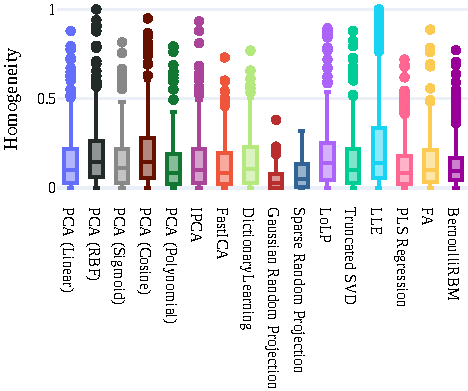
\includegraphics[width=\textwidth]{figures/05/ml/agg_5_homogeneity.pdf}
        \caption{\footnotesize{$k = 5$; homogeneity}}
    \end{subfigure}
    \begin{subfigure}{0.24\textwidth}
        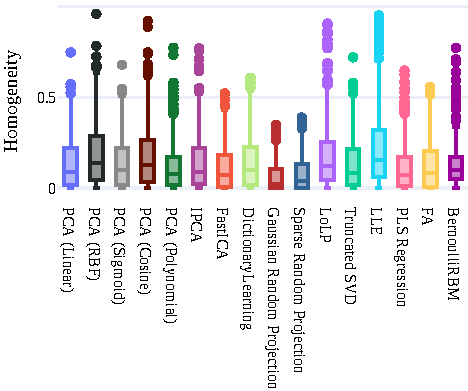
\includegraphics[width=\textwidth]{figures/05/ml/agg_10_homogeneity.pdf}
        \caption{\footnotesize{$k = 10$; homogeneity}}
    \end{subfigure}
    \begin{subfigure}{0.24\textwidth}
        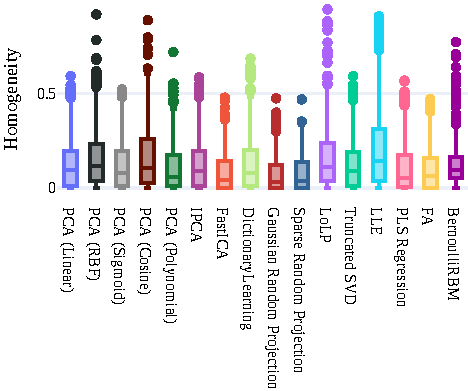
\includegraphics[width=\textwidth]{figures/05/ml/agg_20_homogeneity.pdf}
        \caption{\footnotesize{$k = 20$; homogeneity}}
    \end{subfigure}
    \begin{subfigure}{0.24\textwidth}
        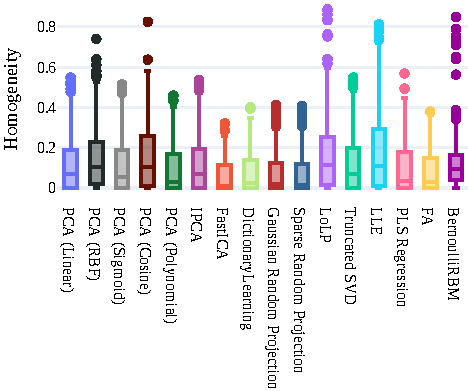
\includegraphics[width=\textwidth]{figures/05/ml/agg_40_homogeneity.pdf}
        \caption{\footnotesize{$k = 40$; homogeneity}}
    \end{subfigure}
    \begin{subfigure}{0.24\textwidth}
        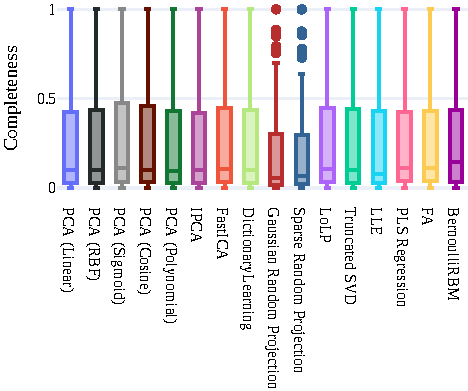
\includegraphics[width=\textwidth]{figures/05/ml/agg_5_completeness.pdf}
        \caption{\footnotesize{$k = 5$; completeness}}
    \end{subfigure}
    \begin{subfigure}{0.24\textwidth}
        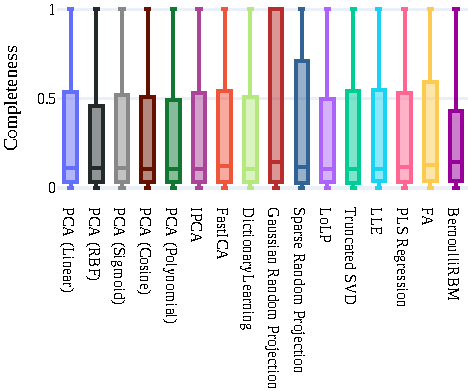
\includegraphics[width=\textwidth]{figures/05/ml/agg_10_completeness.pdf}
        \caption{\footnotesize{$k = 10$; completeness}}
    \end{subfigure}
    \begin{subfigure}{0.24\textwidth}
        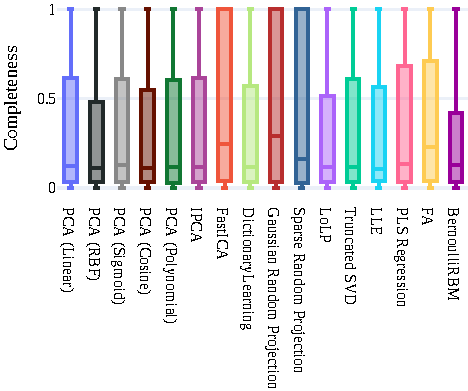
\includegraphics[width=\textwidth]{figures/05/ml/agg_20_completeness.pdf}
        \caption{\footnotesize{$k = 20$; completeness}}
    \end{subfigure}
    \begin{subfigure}{0.24\textwidth}
        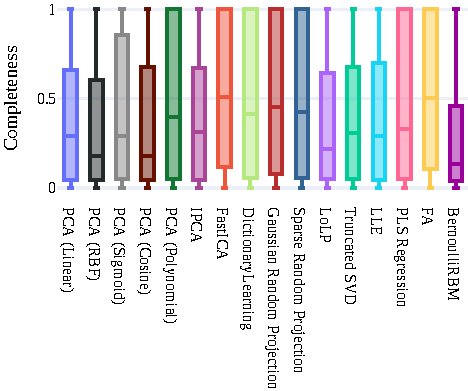
\includegraphics[width=\textwidth]{figures/05/ml/agg_40_completeness.pdf}
        \caption{\footnotesize{$k = 40$; completeness}}
    \end{subfigure}
    % \begin{subfigure}{0.24\textwidth}
    %     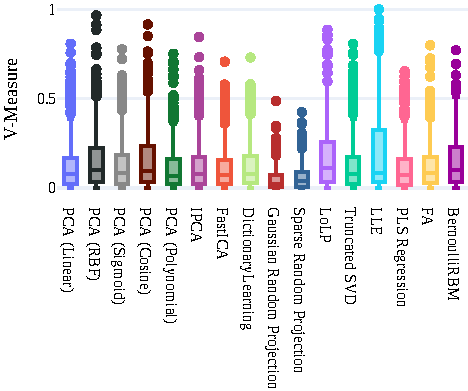
\includegraphics[width=\textwidth]{figures/05/ml/agg_5_v_measure.pdf}
    %     \caption{\tiny{$k$=5 V-Measure}}
    % \end{subfigure}
    % \begin{subfigure}{0.24\textwidth}
    %     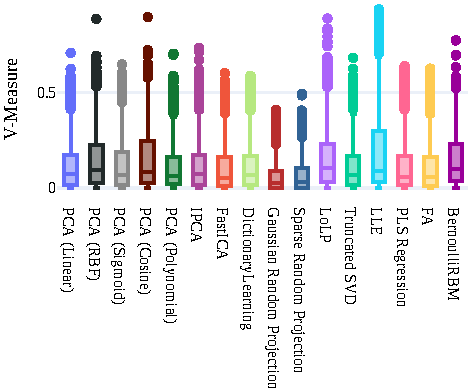
\includegraphics[width=\textwidth]{figures/05/ml/agg_10_v_measure.pdf}
    %     \caption{\tiny{$k$=10 V-Measure}}
    % \end{subfigure}
    % \begin{subfigure}{0.24\textwidth}
    %     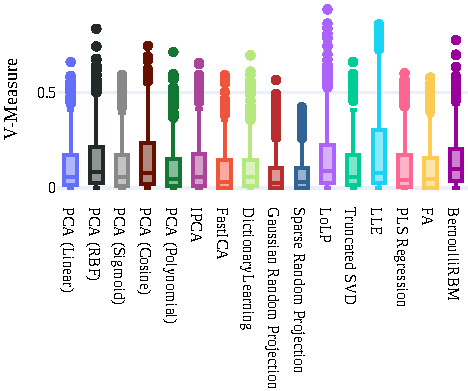
\includegraphics[width=\textwidth]{figures/05/ml/agg_20_v_measure.pdf}
    %     \caption{\tiny{$k$=20 V-Measure}}
    % \end{subfigure}
    % \begin{subfigure}{0.24\textwidth}
    %     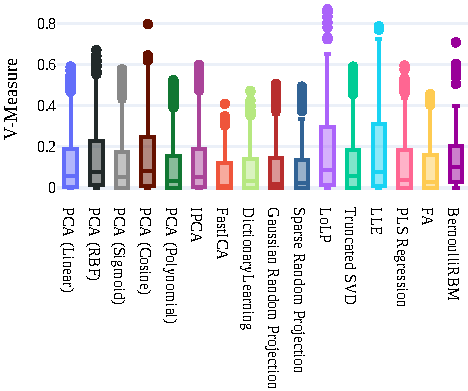
\includegraphics[width=\textwidth]{figures/05/ml/agg_40_v_measure.pdf}
    %     \caption{\tiny{$k$=40 V-Measure}}
    % \end{subfigure}
% \begin{subfigure}[t]{0.8\textwidth}
%         \centering
%         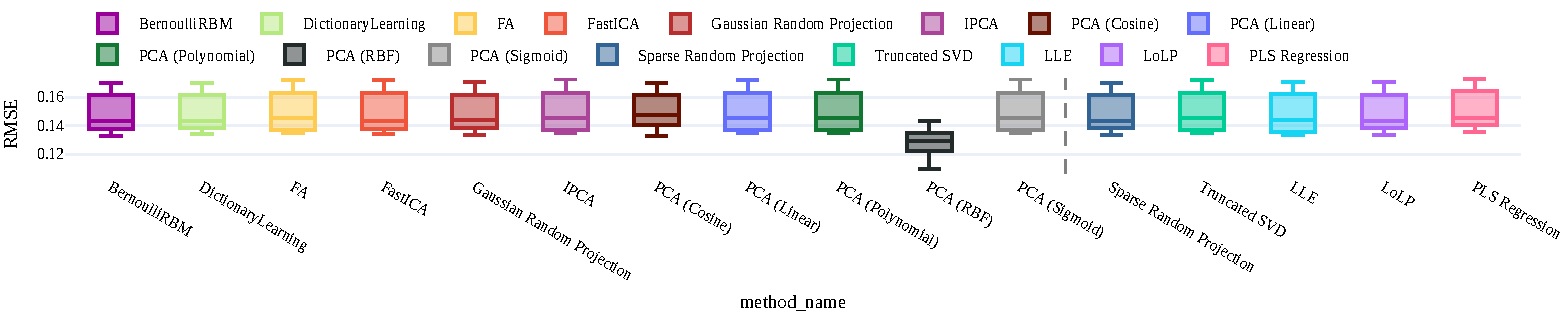
\includegraphics[width=1.0\textwidth,trim={1.5cm 4cm 3.7cm 0.0cm},clip]{figures/05/legend.pdf}
%     \end{subfigure}
\caption{
% \changed{
Performance of different dimensionality reduction methods aggregated across all OpenML~CC-18 datasets, for different target dimensionalities $k$, in terms of (a-d) cluster homogeneity and (e-h) cluster completeness on \textbf{machine learning task 1: clustering ability}; higher is better. Homogeneity measures whether each cluster contains samples from the same true class; we observe very small homogeneity differences between dimensionality reduction methods for different target dimensionalities. Completeness quantifies whether all samples belonging to the same true class are in the same cluster; we observe a slight improvement in performance measured by completeness as the target dimensionality increases.
% }
}
\label{fig:cluster_all_agg}
\end{figure}

We now investigate the effect of input dimensionality by grouping the datasets into three categories based on their number of features: low- (up to 60 features), medium- (60–200 features), and high-dimensional datasets (more than 200 features). The results are presented in \autoref{fig:cluster_homogeneity_dataset_sizes}.
We observe that LLE performs increasingly well on both metrics as the input dimensionality grows, reaching its best performance on medium-dimensional datasets.
% \hh{better: This is possibly due to interference between ...}
% \changed{
This is possibly due to interference between the fact that some dimensions are irrelevant in the large-sized datasets and the estimation of a local neighbourhood.
% }
% This can be explained as irrelevant dimensions in the large dimension datasets may interfere with local neighbourhood estimation.
% \hh{Once again, why `For completeness'?}
% \changed{
With respect to cluster completeness, sparse random projection performs best on medium-dimensional data, whereas Gaussian random projection becomes the strongest method for large input dimensionalities, likely due to its ability to better preserve pairwise distances in high dimensions, consistent with the Johnson–Lindenstrauss effect.
Furthermore, dense Gaussian random projections handle large feature spaces better than sparse ones, avoiding information loss in very high dimensions.

\begin{figure}
\centering
    \begin{subfigure}{0.32\textwidth}
        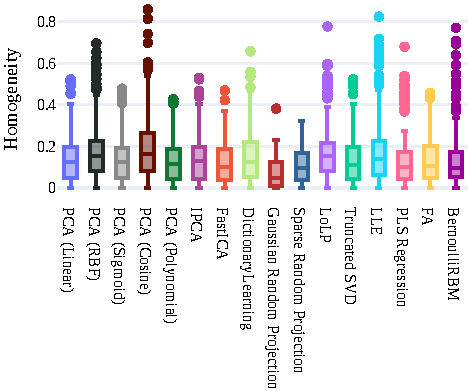
\includegraphics[width=\textwidth]{figures/05/ml/agg_small_5_homogeneity.pdf}
        \caption{Small $D$; homogeneity}
    \end{subfigure}
    \begin{subfigure}{0.32\textwidth}
        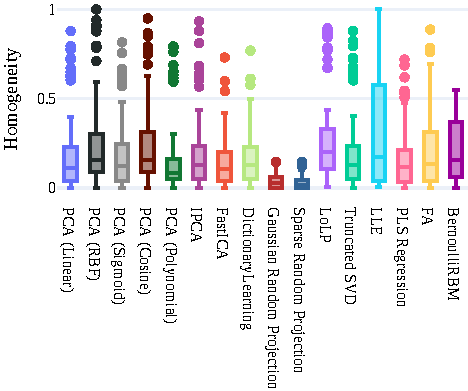
\includegraphics[width=\textwidth]{figures/05/ml/agg_medium_5_homogeneity.pdf}
        \caption{Medium $D$; homogeneity}
    \end{subfigure}
    \begin{subfigure}{0.32\textwidth}
        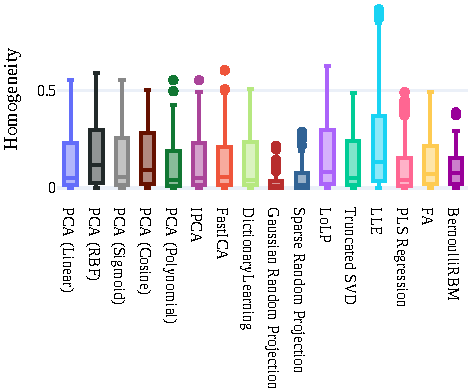
\includegraphics[width=\textwidth]{figures/05/ml/agg_large_5_homogeneity.pdf}
        \caption{Large $D$; homogeneity}
    \end{subfigure}
    \begin{subfigure}{0.32\textwidth}
        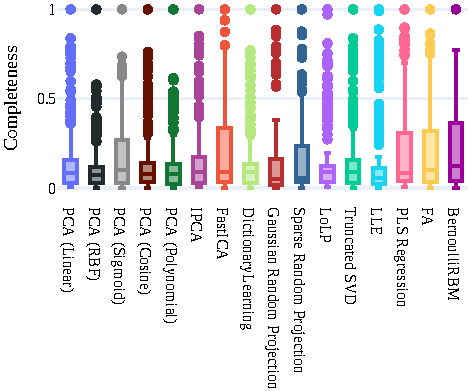
\includegraphics[width=\textwidth]{figures/05/ml/agg_small_5_completeness.pdf}
        \caption{Small $D$; completeness}
    \end{subfigure}
    \begin{subfigure}{0.32\textwidth}
        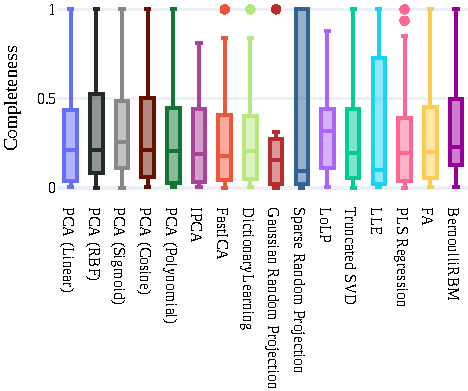
\includegraphics[width=\textwidth]{figures/05/ml/agg_medium_5_completeness.pdf}
        \caption{Medium $D$; completeness}
    \end{subfigure}
    \begin{subfigure}{0.32\textwidth}
        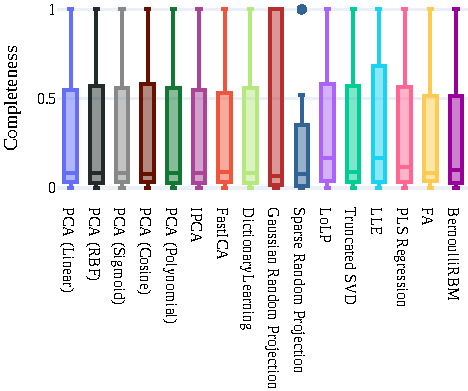
\includegraphics[width=\textwidth]{figures/05/ml/agg_large_5_completeness.pdf}
        \caption{Large $D$; completeness}
    \end{subfigure}
    \begin{subfigure}{0.32\textwidth}
    %     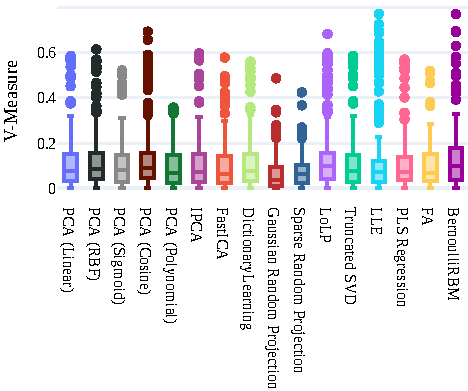
\includegraphics[width=\textwidth]{figures/05/ml/agg_small_5_v_measure.pdf}
    %     \caption{\tiny{$k$=5 }}
    % \end{subfigure}
    % \begin{subfigure}{0.24\textwidth}
    %     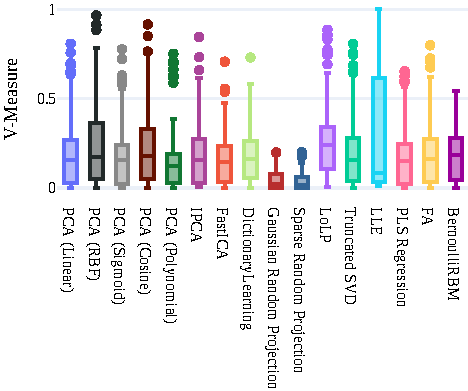
\includegraphics[width=\textwidth]{figures/05/ml/agg_medium_5_v_measure.pdf}
    %     \caption{\tiny{$k$=10 }}
    % \end{subfigure}
    % \begin{subfigure}{0.24\textwidth}
    %     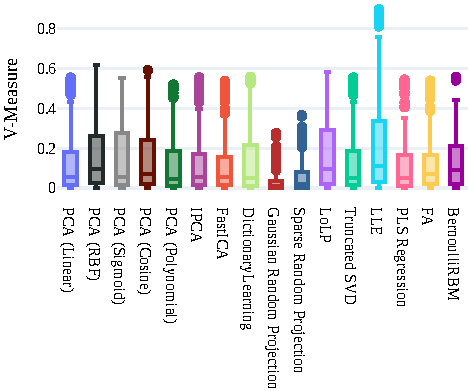
\includegraphics[width=\textwidth]{figures/05/ml/agg_large_5_v_measure.pdf}
    %     \caption{\tiny{$k$=20 }}
    \end{subfigure}
% \begin{subfigure}[t]{0.8\textwidth}
%         \centering
%         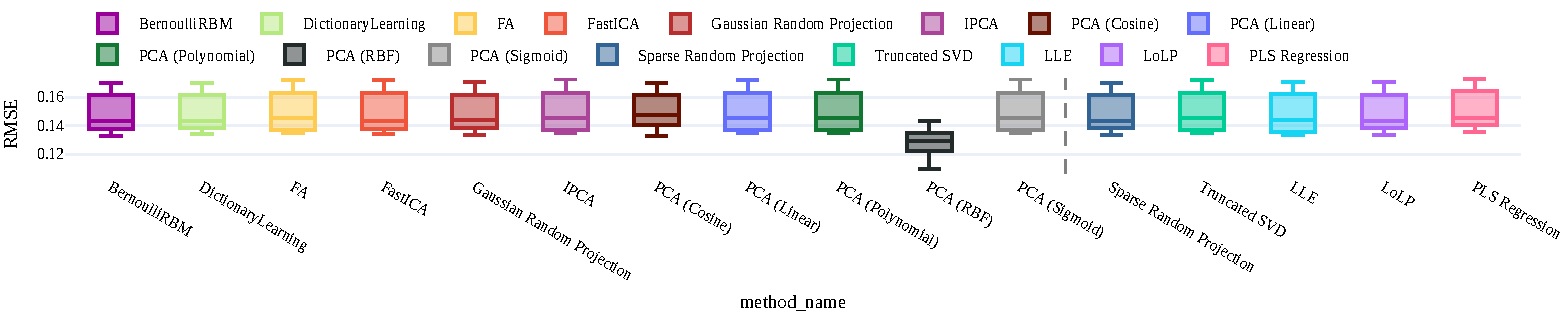
\includegraphics[width=1.0\textwidth,trim={1.5cm 4cm 3.7cm 0.0cm},clip]{figures/05/legend.pdf}
%     \end{subfigure}
\caption{
% \changed{
Performance of different dimensionality reduction methods on low-, medium- and high-dimensional OpenML~CC-18 datasets, all reduced to target dimensionality $k = 5$, in terms of (a-c) cluster homogeneity and (d-f) cluster completeness on \textbf{machine learning task 1: clustering ability}; higher is better. We observe a slightly larger improvement in completeness than in homogeneity as the dataset dimensionality increases.
% }
% \todo{if we can please have 2 rows x 3 columns s.t. homogeneity is in the first row and completeness in the second row? Also for the following figures analogously}
}
\label{fig:cluster_homogeneity_dataset_sizes}
\end{figure}
% }


\subsubsection*{Machine learning task 2: Tabular classification accuracy}

% \changed{
% \changed{
For the supervised machine learning task (\emph{i.e.,} prediction), 
% }
we begin by analysing the results aggregated across all datasets and different machine learning models (random forest, gradient boosting, \gls{mlp}) for varying target dimensionalities $k$, as shown in \autoref{fig:ml_pred_all}.
Across all models and methods, we observe that accuracy increases with the target dimensionality. 
% -- \er{Stupid question, is this type of dash correct?} 
% \changed{
In other words,
% }
% that is, 
performance is lowest at $k=5$ and highest at $k=40$. 
This observation indicates that higher-dimensional projections retain more task-relevant information, allowing downstream models to make more accurate predictions.

Interestingly, while Gaussian and sparse random projection performed relatively well in the clustering task (particularly for cluster completeness), they rank among the worst-performing methods in the prediction task, only outperforming Bernoulli RBM. This suggests that although random projections preserve geometric structure, they do not necessarily retain the discriminative information required for predictive modelling.
Overall, while most methods achieve comparable accuracy, LoLP consistently performs best. This outcome is expected, as LoLP is explicitly designed to enhance predictive performance in machine learning settings, confirming its suitability for supervised downstream tasks.


\begin{figure}
\centering
    \begin{subfigure}{0.24\textwidth}
        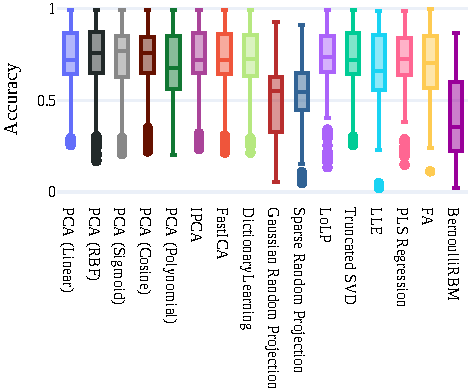
\includegraphics[width=\textwidth]{figures/05/ml/agg_5_rf_acc.pdf}
        \caption{\footnotesize Random Forest; $k = 5$}
    \end{subfigure}
    \begin{subfigure}{0.24\textwidth}
        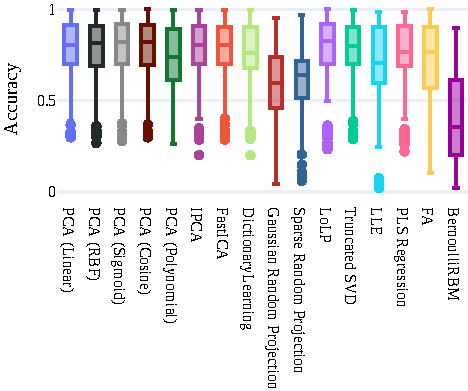
\includegraphics[width=\textwidth]{figures/05/ml/agg_10_rf_acc.pdf}
        \caption{\footnotesize Random Forest; $k = 10$}
    \end{subfigure}
    \begin{subfigure}{0.24\textwidth}
        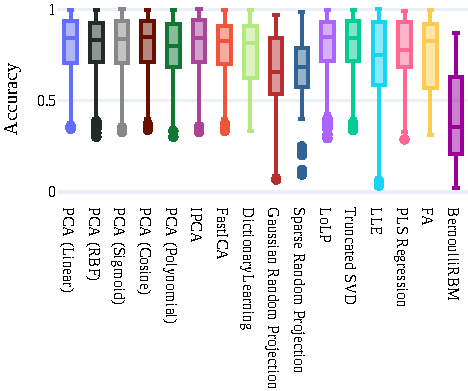
\includegraphics[width=\textwidth]{figures/05/ml/agg_20_rf_acc.pdf}
        \caption{\footnotesize Random Forest; $k = 20$}
    \end{subfigure}
    \begin{subfigure}{0.24\textwidth}
        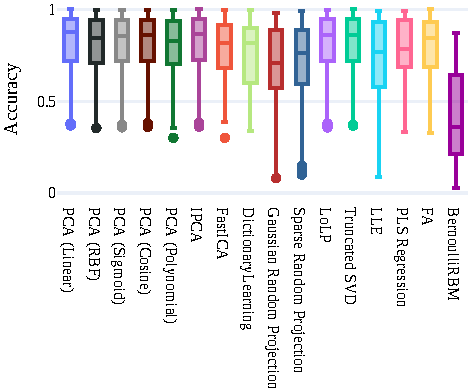
\includegraphics[width=\textwidth]{figures/05/ml/agg_40_rf_acc.pdf}
        \caption{\footnotesize Random Forest; $k = 40$}
    \end{subfigure}
    \begin{subfigure}{0.24\textwidth}
        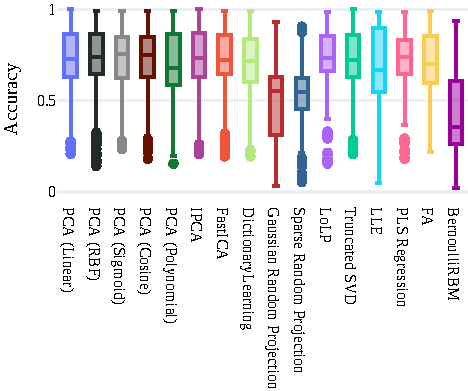
\includegraphics[width=\textwidth]{figures/05/ml/agg_5_gb_acc.pdf}
        \caption{\footnotesize Gradient Boosting; $k = 5$}
    \end{subfigure}
    \begin{subfigure}{0.24\textwidth}
        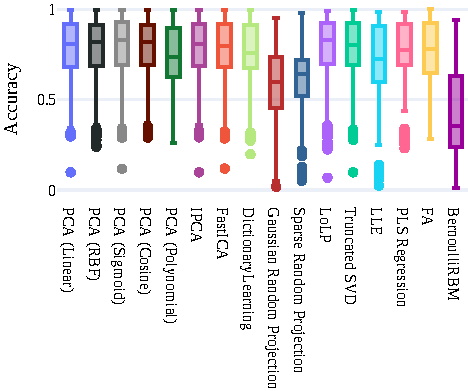
\includegraphics[width=\textwidth]{figures/05/ml/agg_10_gb_acc.pdf}
        \caption{\footnotesize Gradient Boosting; $k = 10$}
    \end{subfigure}
    \begin{subfigure}{0.24\textwidth}
        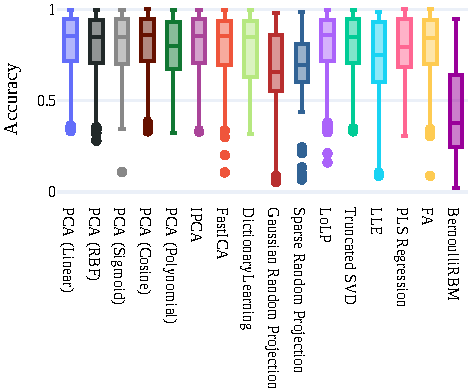
\includegraphics[width=\textwidth]{figures/05/ml/agg_20_gb_acc.pdf}
        \caption{\footnotesize Gradient Boosting; $k = 20$}
    \end{subfigure}
    \begin{subfigure}{0.24\textwidth}
        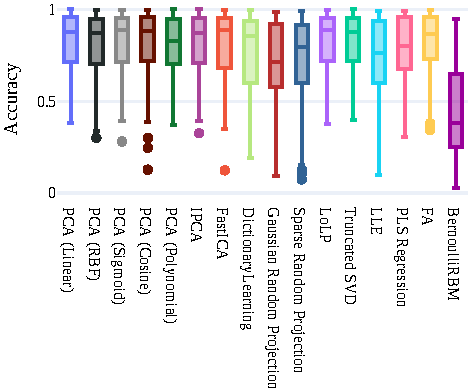
\includegraphics[width=\textwidth]{figures/05/ml/agg_40_gb_acc.pdf}
        \caption{\footnotesize Gradient Boosting; $k = 40$}
    \end{subfigure}
    \begin{subfigure}{0.24\textwidth}
        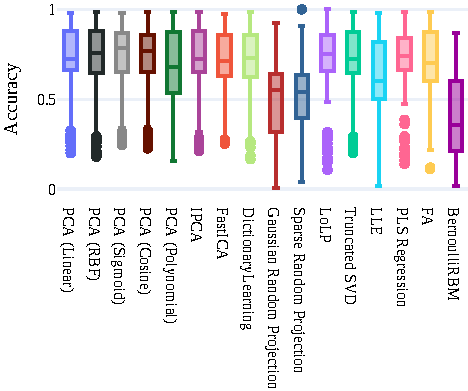
\includegraphics[width=\textwidth]{figures/05/ml/agg_5_mlp_acc.pdf}
        \caption{\footnotesize \gls{mlp}; $k = 5$}
    \end{subfigure}
    \begin{subfigure}{0.24\textwidth}
        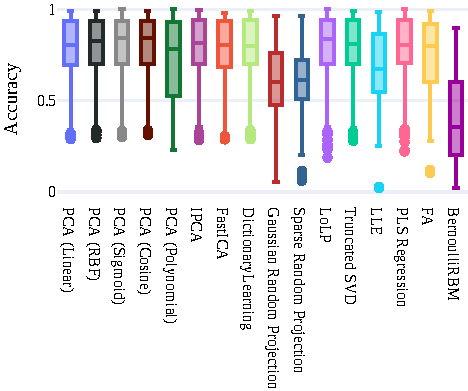
\includegraphics[width=\textwidth]{figures/05/ml/agg_10_mlp_acc.pdf}
        \caption{\footnotesize \gls{mlp}; $k = 10$}
    \end{subfigure}
    \begin{subfigure}{0.24\textwidth}
        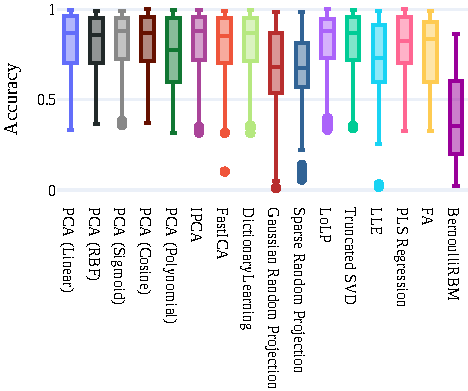
\includegraphics[width=\textwidth]{figures/05/ml/agg_20_mlp_acc.pdf}
        \caption{\footnotesize \gls{mlp}; $k = 20$}
    \end{subfigure}
    \begin{subfigure}{0.24\textwidth}
        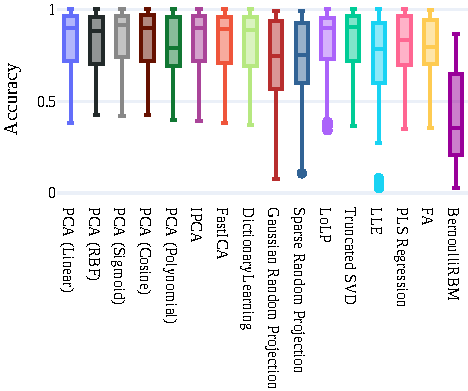
\includegraphics[width=\textwidth]{figures/05/ml/agg_40_mlp_acc.pdf}
        \caption{\footnotesize \gls{mlp}; $k = 40$}
    \end{subfigure}
% \begin{subfigure}[t]{0.8\textwidth}
%         \centering
%         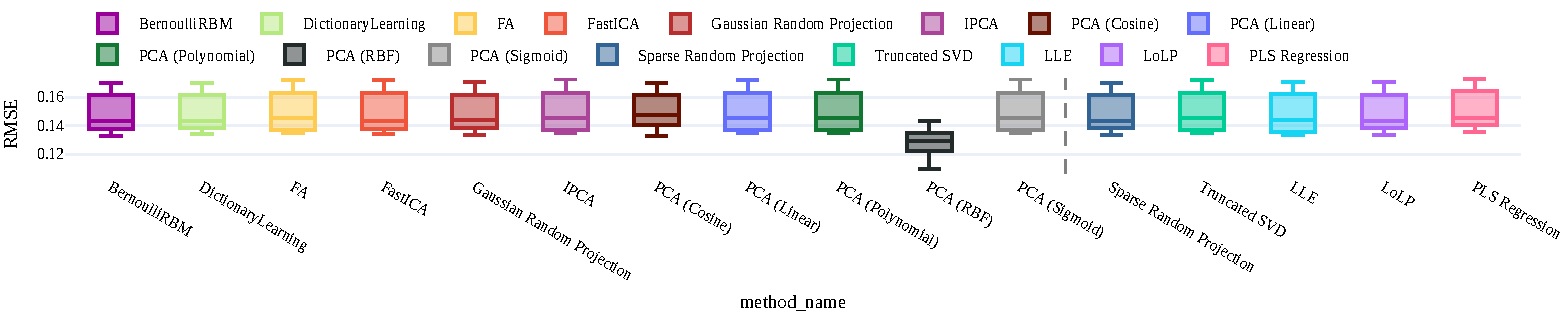
\includegraphics[width=1.0\textwidth,trim={1.5cm 4cm 3.7cm 0.0cm},clip]{figures/05/legend.pdf}
%     \end{subfigure}
\caption{
% \changed{
Performance of different dimensionality reduction methods aggregated across all OpenML~CC-18 datasets, for different target dimensionalities $k$ and for different machine learning models used for classification (random forest, gradient boosting, \gls{mlp}), in terms of accuracy on \textbf{machine learning task 2: tabular classification accuracy}; higher is better. Bernoulli RBM performs consistently bad across all settings, followed by Gaussian and sparse random projections, while LoLP exhibits a consistent slight performance edge over other methods.
% }
}
\label{fig:ml_pred_all}
\end{figure}

We conclude our analysis of the machine learning tasks by examining the results of the prediction task across different dataset sizes, following the same procedure as for the clustering task. We fix the target dimensionality to $k=5$.
% \hh{You often write `dimension' when you mean `dimensionality' -- these two are different and should not be confused with each other.}
We first observe that Bernoulli RBM, Gaussian and sparse random projections show strongly degraded performance as the number of features increases. Even on the low-dimensional datasets, these methods already underperform compared to other approaches, suggesting that they increasingly fail to preserve essential information needed for predictive modelling as dataset dimensionality increases.
In contrast, PCA (Linear) and PCA (Polynomial) perform better than other PCA variants on low-dimensional datasets. This behaviour likely reflects that linear and low-order polynomial relationships are sufficient to capture the main predictive variance in smaller feature spaces, while more complex kernels (such as RBF or Cosine) become beneficial only in higher-dimensional spaces.

\begin{figure}
\centering
    \begin{subfigure}{0.32\textwidth}
        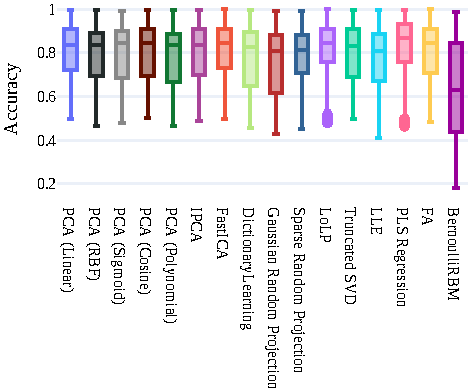
\includegraphics[width=\textwidth]{figures/05/ml/agg_small_5_rf_acc.pdf}
        \caption{Small $D$; Random Forest}
    \end{subfigure}
    \begin{subfigure}{0.32\textwidth}
        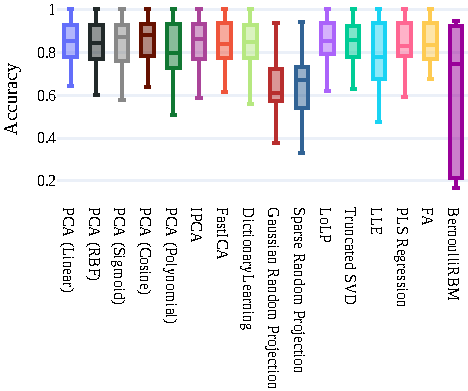
\includegraphics[width=\textwidth]{figures/05/ml/agg_medium_5_rf_acc.pdf}
        \caption{Medium $D$; Random Forest}
    \end{subfigure}
    \begin{subfigure}{0.32\textwidth}
        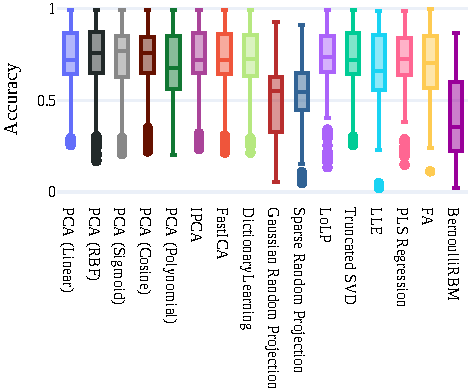
\includegraphics[width=\textwidth]{figures/05/ml/agg_large_5_rf_acc.pdf}
        \caption{Large $D$; Random Forest}
    \end{subfigure}
    \begin{subfigure}{0.32\textwidth}
        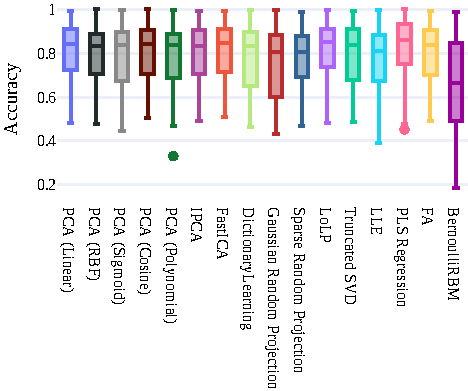
\includegraphics[width=\textwidth]{figures/05/ml/agg_small_5_gb_acc.pdf}
        \caption{Small $D$; Gradient Boosting}
    \end{subfigure}
    \begin{subfigure}{0.32\textwidth}
        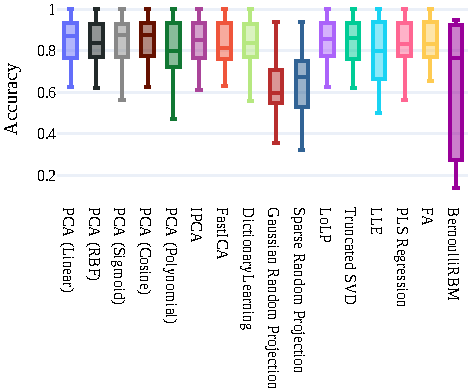
\includegraphics[width=\textwidth]{figures/05/ml/agg_medium_5_gb_acc.pdf}
        \caption{Medium $D$; Gradient Boosting}
    \end{subfigure}
    \begin{subfigure}{0.32\textwidth}
        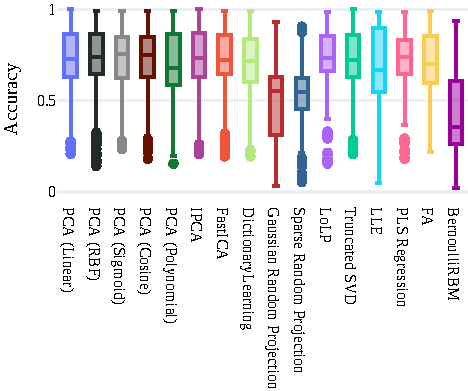
\includegraphics[width=\textwidth]{figures/05/ml/agg_large_5_gb_acc.pdf}
        \caption{Large $D$; Gradient Boosting}
    \end{subfigure}
    \begin{subfigure}{0.32\textwidth}
        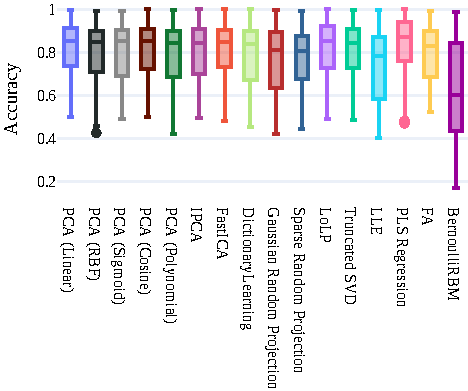
\includegraphics[width=\textwidth]{figures/05/ml/agg_small_5_mlp_acc.pdf}
        \caption{Small $D$; \gls{mlp}}
    \end{subfigure}
    \begin{subfigure}{0.32\textwidth}
        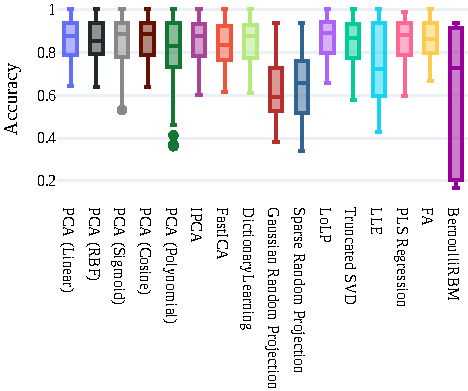
\includegraphics[width=\textwidth]{figures/05/ml/agg_medium_5_mlp_acc.pdf}
        \caption{Medium $D$; \gls{mlp}}
    \end{subfigure}
    \begin{subfigure}{0.32\textwidth}
        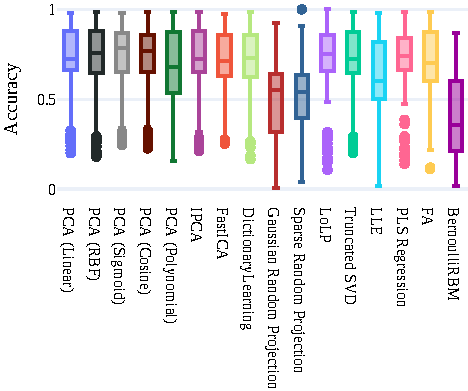
\includegraphics[width=\textwidth]{figures/05/ml/agg_large_5_mlp_acc.pdf}
        \caption{Large $D$; \gls{mlp}}
    \end{subfigure}

% \begin{subfigure}[t]{0.8\textwidth}
%         \centering
%         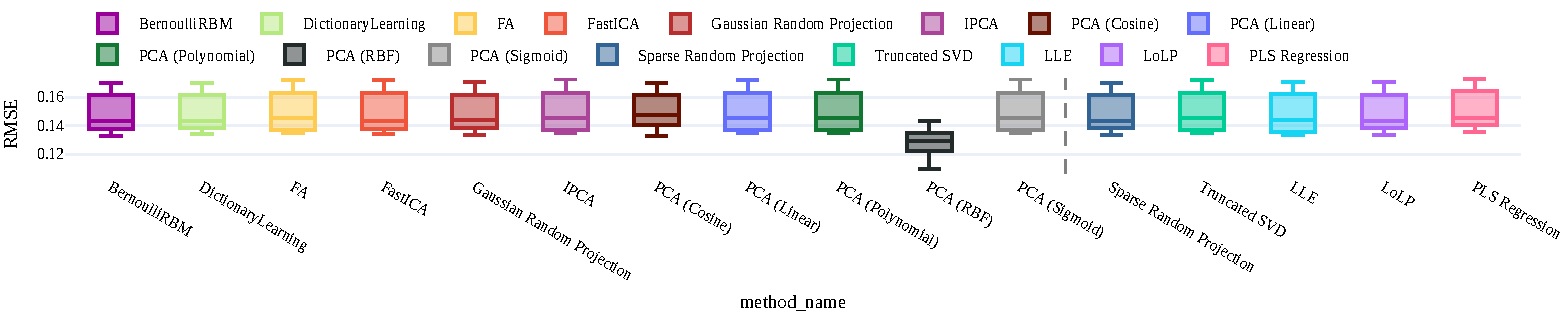
\includegraphics[width=1.0\textwidth,trim={1.5cm 4cm 3.7cm 0.0cm},clip]{figures/05/legend.pdf}
%     \end{subfigure}
\caption{
% \changed{
Performance of different dimensionality reduction methods on low-, medium- and high-dimensional OpenML~CC-18 datasets, all reduced to target dimensionality $k = 5$, in terms of accuracy on \textbf{machine learning task 2: tabular classification accuracy}, where classification is done using different machine learning models (random forest, gradient boosting, \gls{mlp}); higher is better. The performance of Bernoulli RBM and Gaussian and sparse random projection degrades even further as the dataset dimensionality increases, regardless of the machine learning model used for classification. The differences induced by the choice of the machine learning model are generally negligible for low-, medium- and high-dimensional datasets alike.
% }
}
\label{fig:ml_pred_sizes}
\end{figure}

% }
\subsection{Black-box optimisation tasks}
\label{sec:res-bbo}

\subsubsection*{Black-box optimisation task 1: Target function approximation}

% \changed{

% \aj{add info about aggregation of the results, weighting the RMSE}
% \aj{this i need to rewrite and we need to decide on which figures to keep for BBO tasks}

\begin{figure}
    \centering
    \begin{subfigure}[t]{0.24\textwidth}
        \centering
        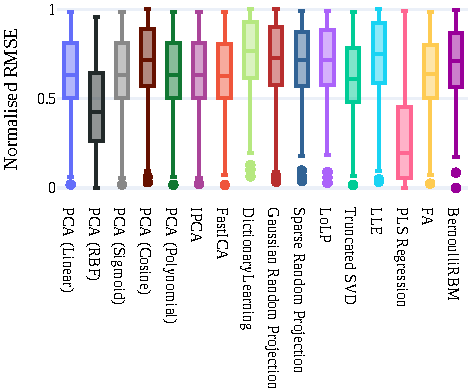
\includegraphics[width=\textwidth]{figures/05/epm/agg_sample_red_inpt_100_120_5.pdf}
        \caption{$k=5$}
    \end{subfigure}
    \begin{subfigure}[t]{0.24\textwidth}
        \centering
        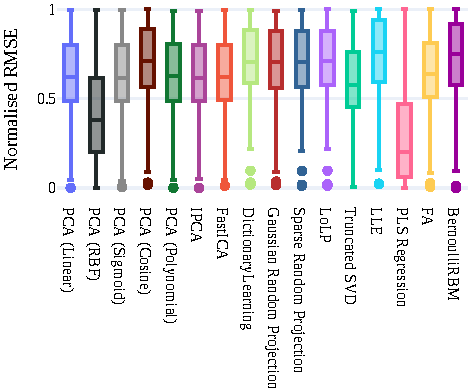
\includegraphics[width=\textwidth]{figures/05/epm/agg_sample_red_inpt_100_120_10.pdf}
        \caption{$k=10$}
    \end{subfigure}
    \begin{subfigure}[t]{0.24\textwidth}
        \centering
        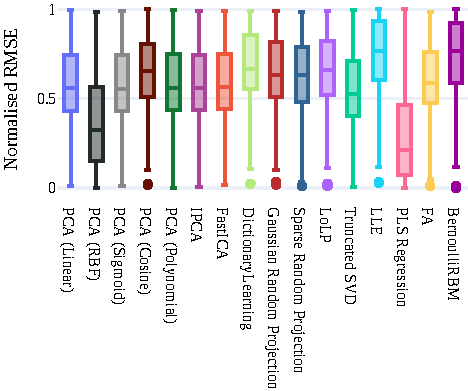
\includegraphics[width=\textwidth]{figures/05/epm/agg_sample_red_inpt_100_120_20.pdf}
        \caption{$k=20$}
    \end{subfigure}
    \begin{subfigure}[t]{0.24\textwidth}
        \centering
        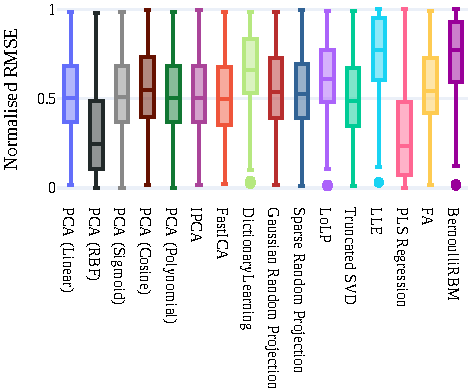
\includegraphics[width=\textwidth]{figures/05/epm/agg_sample_red_inpt_100_120_40.pdf}
        \caption{$k=40$}
    \end{subfigure}
    \caption{
    % \changed{
    Performance of different dimensionality reduction methods aggregated across synthetic benchmark problems for different target dimensionalities $k$, with input dimensionality $D = 120$ and initial sample size $N = 100$, in terms of min-max normalised mean \gls{rmse} on \textbf{black-box optimisation task 1: target function approximation}; lower is better. 
    PLS regression consistently performs best across different target dimensionalities, and is closely followed by PCA (RBF) for the highest target dimensionality.
    % Aggregated and min-max normalised mean normalised RMSE of the methods across all \emph{synthetic} problems for input dimension $120$, $100$ initial samples and different target dimensions.
    % \er{Rank is wrong, this should be mean normalized RMSE.}
    % }
    }
    \label{fig:res-bbo-task1_red_dim_inpt_dim}
\end{figure}

% \changed{
We focus on a selection of representative aggregated results to simplify analysis.
We start by looking into the results on synthetic benchmarks for black-box optimisation task 1.
% }
% \hh{You just focus the discussion on these, right?}
First, we examine the effect of varying the target dimensionality $k$ in \autoref{fig:res-bbo-task1_red_dim_inpt_dim}, keeping the input dimensionality fixed at $D = 120$ and the initial sample size at $N = 100$.
Across all target dimensionalities, and particularly in the low-dimensional setting, PLS regression consistently performs best. 
This aligns with expectations, as PLS components are explicitly optimised to maximise the predictive power of the target variables, which is especially suitable when dimensionality reduction is used as a preprocessing step for regression. 
% In other words, the strong performance of PLS regression reflects that this task is fundamentally evaluating predictive power.
As the target dimensionality increases, PCA (RBF) gradually catches up and eventually performs on par with PLS regression. More generally, all PCA variants improve their relative performance with higher target dimensionalities, likely because higher-dimensional projections preserve more variance and structure from the original data, even without explicit supervision.

% Taken together, our results highlight an important distinction between supervised and unsupervised dimensionality reduction. In the predictive task (black-box optimisation task 1), PLSRegression excels at low target dimensions because it explicitly optimises components for predicting the target variables, while PCA variants only match its performance once the target dimension is sufficiently high, allowing them to retain sufficient variance and structure for effective prediction. In contrast, in the clustering experiments, which are unsupervised, methods that preserve local structure (e.g., LLE) or capture non-linear relationships (e.g., PCA with RBF or Cosine kernels) tend to perform better. Random projection methods, particularly at higher dimensions, also show improvements due to the Johnson–Lindenstrauss effect, which preserves pairwise distances and cluster structure. Overall, these findings suggest that the task objective strongly shapes which dimensionality reduction method is most effective: supervised tasks favour methods aligned with predictive power, while unsupervised tasks benefit from methods that preserve geometric or topological structure.

\begin{figure}
\begin{subfigure}[t]{0.32\textwidth}
        \centering
        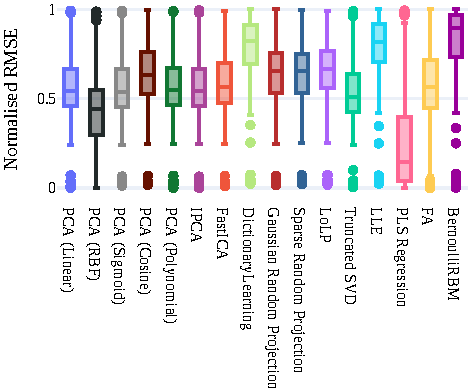
\includegraphics[width=\textwidth]{figures/05/epm/agg_sample_red_inpt_100_40_20.pdf}
        \caption{$D=40$}
    \end{subfigure}
    \begin{subfigure}[t]{0.32\textwidth}
        \centering
        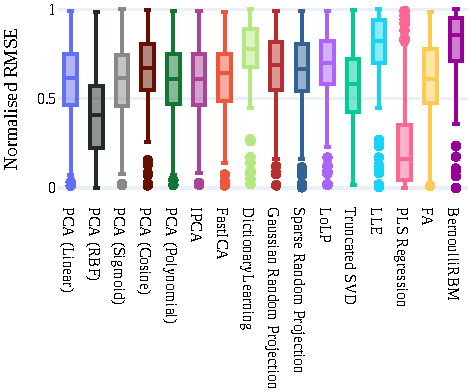
\includegraphics[width=\textwidth]{figures/05/epm/agg_sample_red_inpt_100_60_20.pdf}
        \caption{$D=60$}
    \end{subfigure}
    \begin{subfigure}[t]{0.32\textwidth}
        \centering
        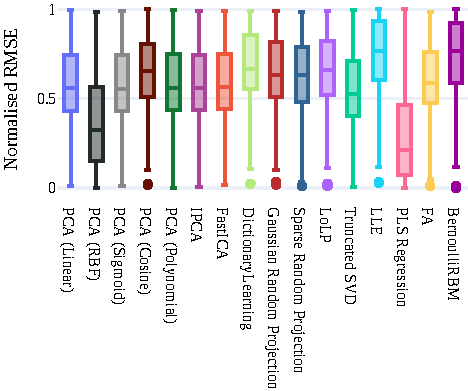
\includegraphics[width=\textwidth]{figures/05/epm/agg_sample_red_inpt_100_120_20.pdf}
        \caption{$D=120$}
    \end{subfigure}
    \begin{subfigure}[t]{0.32\textwidth}
        \centering
        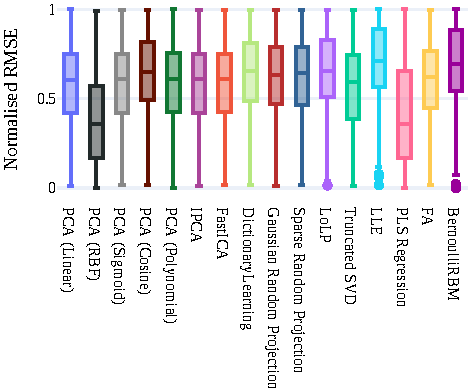
\includegraphics[width=\textwidth]{figures/05/epm/agg_sample_red_inpt_100_240_20.pdf}
        \caption{$D=240$}
    \end{subfigure}
    \begin{subfigure}[t]{0.32\textwidth}
        \centering
        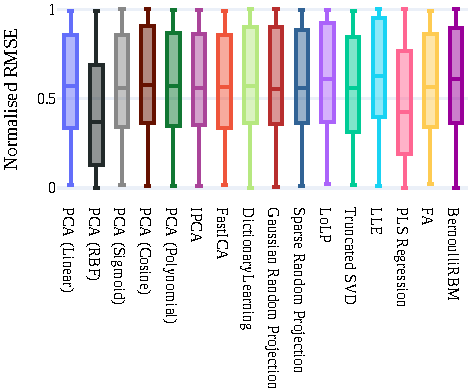
\includegraphics[width=\textwidth]{figures/05/epm/agg_sample_red_inpt_100_500_20.pdf}
        \caption{$D=500$}
    \end{subfigure}
    \begin{subfigure}[t]{0.32\textwidth}
        \centering
        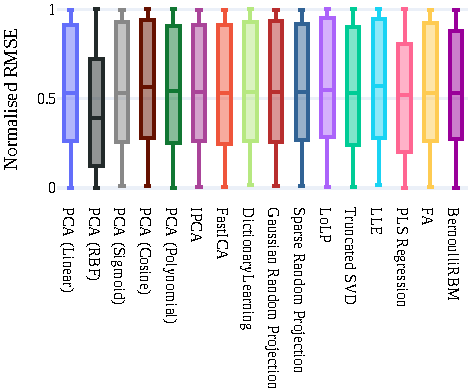
\includegraphics[width=\textwidth]{figures/05/epm/agg_sample_red_inpt_100_1000_20.pdf}
        \caption{$D=1000$}
    \end{subfigure}
    \hspace{0.2cm}
    \begin{subfigure}[t]{0.8\textwidth}
        \centering
        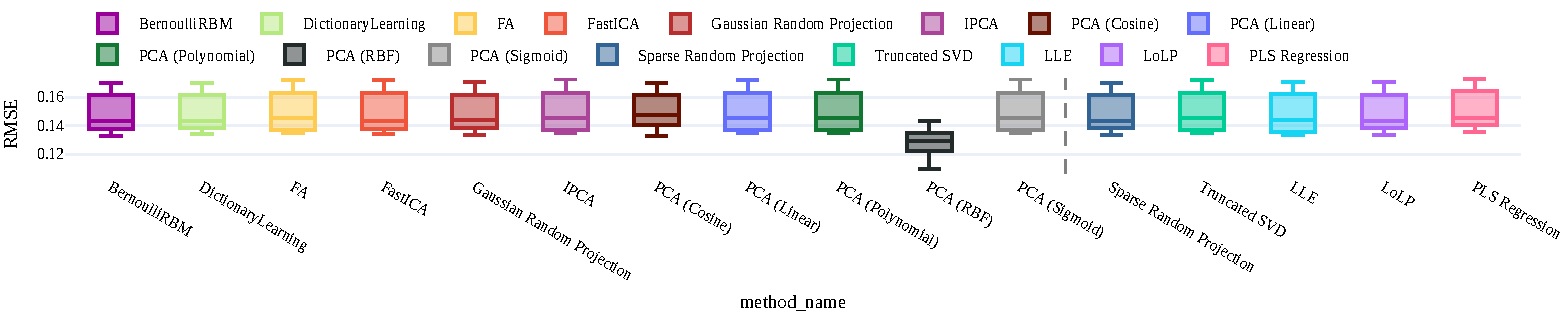
\includegraphics[width=1.0\textwidth,trim={1.5cm 4cm 3.7cm 0.0cm},clip]{figures/05/legend.pdf}
    \end{subfigure}
    \caption{
    % \changed{
    Performance of different dimensionality reduction methods aggregated across synthetic benchmark problems for different input dimensionalities $D$, with target dimensionality $k = 20$ and initial sample size $N = 100$, in terms of min-max normalised mean \gls{rmse} on \textbf{black-box optimisation task 1: target function approximation}; lower is better. 
    The variance increases with input dimensionality; PLS regression is a dominant method for lower-dimensional inputs (a-c), but is outperformed by PCA (RBF) for higher-dimensional inputs (d-f).
    % (a) Aggregated and min-max normalised mean ranks of the methods across all \emph{synthetic} problems for different dimensions with $100$ initial samples, target dimension $20$.\er{Rank is wrong, this should be mean normalized RMSE.}
    % }
    }
    \label{fig:res-bbo-task1_inpt_dim}
\end{figure}

% \hh{incomplete sentence??}
% \changed{
Second, we look into the effect of varying the input dimensionality $D$, keeping the target dimensionality fixed at $k = 20$ and the initial sample size at $N = 100$. This is illustrated in~\autoref{fig:res-bbo-task1_inpt_dim}.
% }
% k=20 and the sample size at 100 (see \autoref{fig:res-bbo-task1_inpt_dim}). 
As expected, the variance of all methods decreases with lower input dimensionality, reflecting the reduced complexity of the search space. In this setting (up to ~120 input dimensions), PLS regression consistently outperforms other methods, leveraging its ability to extract components that are directly predictive of the targets. Conversely, for higher input dimensionalities, PCA (RBF) becomes the dominant method, likely because it captures more of the underlying variance and non-linear structure that PLS regression cannot exploit efficiently in very high-dimensional spaces. Together with previous findings, this suggests that PLS regression is best when both input and output dimensions are small, while PCA (RBF) is more suitable for high-dimensional settings.



\begin{figure}
    \centering
    \begin{subfigure}[t]{0.24\textwidth}
        \centering
        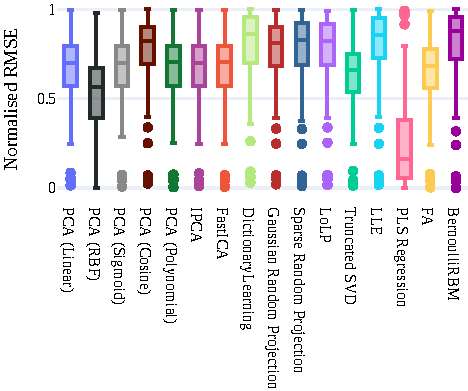
\includegraphics[width=\textwidth]{figures/05/epm/agg_sample_red_inpt_100_40_5}
        \caption{\footnotesize$D = 40, k = 5, N = 100$}
    \end{subfigure}
    \begin{subfigure}[t]{0.24\textwidth}
        \centering
        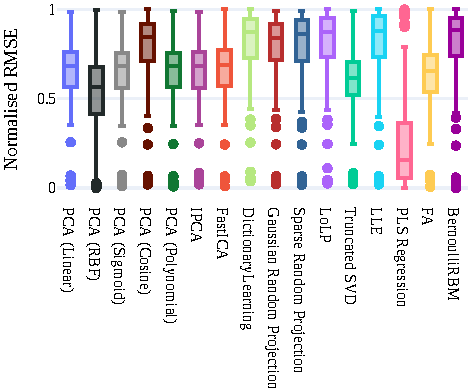
\includegraphics[width=\textwidth]{figures/05/epm/agg_sample_red_inpt_200_40_5.pdf}
        \caption{\footnotesize$D = 40, k = 5, N = 200$}
    \end{subfigure}
    \begin{subfigure}[t]{0.24\textwidth}
        \centering
        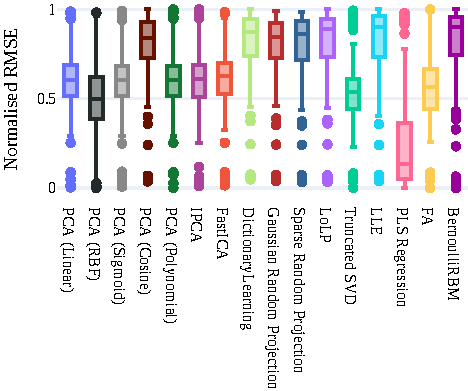
\includegraphics[width=\textwidth]{figures/05/epm/agg_sample_red_inpt_500_40_5.pdf}
        \caption{\footnotesize$D = 40, k = 5, N = 500$}
    \end{subfigure}
    \begin{subfigure}[t]{0.24\textwidth}
        \centering
        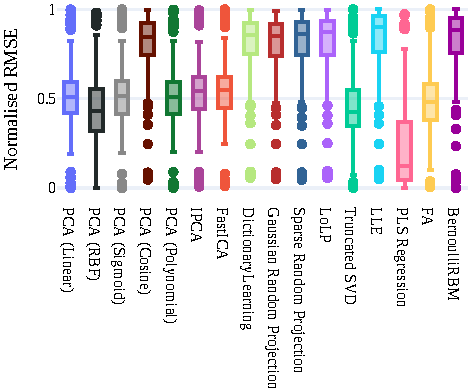
\includegraphics[width=\textwidth]{figures/05/epm/agg_sample_red_inpt_1000_40_5.pdf}
        \caption{\footnotesize$D = 40, k = 5, N = 1000$}
    \end{subfigure}
    \begin{subfigure}[t]{0.24\textwidth}
        \centering
        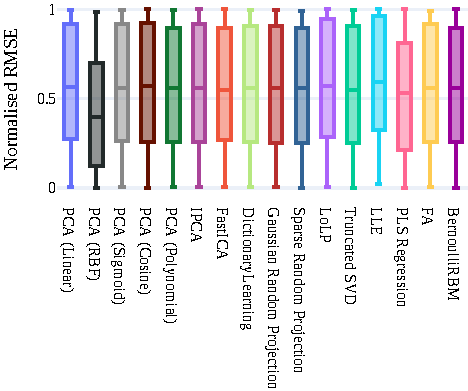
\includegraphics[width=\textwidth]{figures/05/epm/agg_sample_red_inpt_100_1000_40.pdf}
        \caption{\footnotesize$D = 1000, k = 40, N = 100$}
    \end{subfigure}
    \begin{subfigure}[t]{0.24\textwidth}
        \centering
        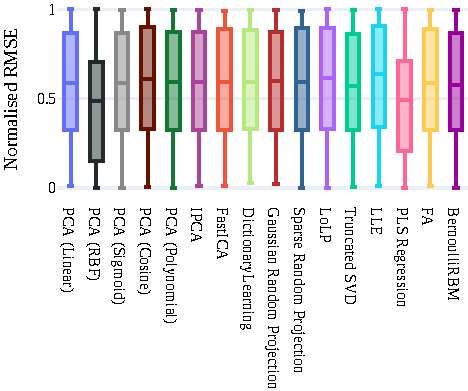
\includegraphics[width=\textwidth]{figures/05/epm/agg_sample_red_inpt_200_1000_40.pdf}
        \caption{\footnotesize$D = 1000, k = 40, N = 200$}
    \end{subfigure}
    \begin{subfigure}[t]{0.24\textwidth}
        \centering
        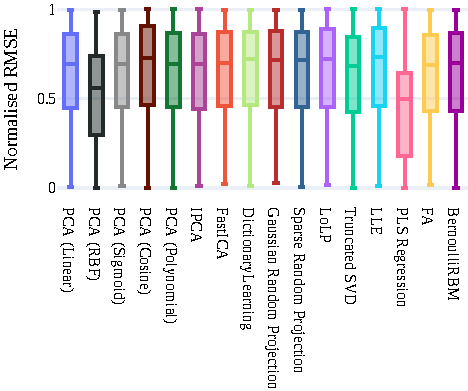
\includegraphics[width=\textwidth]{figures/05/epm/agg_sample_red_inpt_500_1000_40.pdf}
        \caption{\footnotesize$D = 1000, k = 40, N = 500$}
    \end{subfigure}
    \begin{subfigure}[t]{0.24\textwidth}
        \centering
        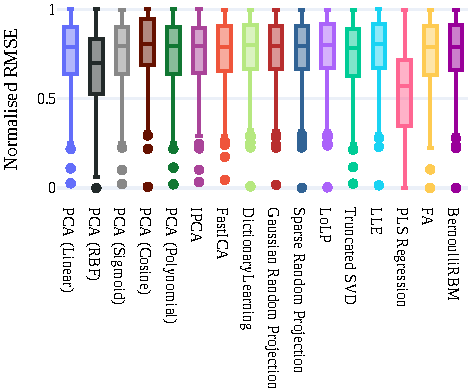
\includegraphics[width=\textwidth]{figures/05/epm/agg_sample_red_inpt_1000_1000_40.pdf}
        \caption{\footnotesize$D = 1000, k = 40, N = 1000$}
    \end{subfigure}
    \hspace{0.2cm}
    \begin{subfigure}[t]{0.8\textwidth}
        \centering
        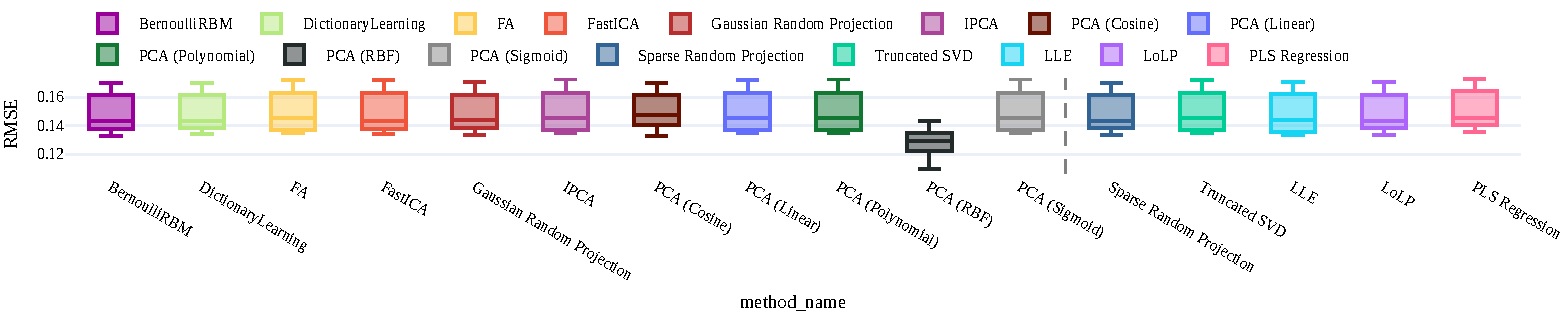
\includegraphics[width=1.0\textwidth,trim={1.5cm 4cm 3.7cm 0.0cm},clip]{figures/05/legend.pdf}
    \end{subfigure}
    \caption{
    % \changed{
    Performance of different dimensionality reduction methods aggregated across synthetic benchmark problems for different initial sample sizes $N$ in two settings: (a-d) with input dimensionality $D = 40$ and target dimensionality $k = 5$, and (e-h) with input dimensionality $D = 1000$ and target dimensionality $k = 40$, in terms of min-max normalised mean \gls{rmse} on \textbf{black-box optimisation task 1: target function approximation}; lower is better.
    Initial sample size has almost no effect when the dimensionality reduction is performed from an already low-dimensional space into an even lower-dimensional one. On the other hand, for a more drastic dimensionality reduction from a very high-dimensional space into a relatively low-dimensional one, a large initial sample size is necessary for accurate target function approximation. 
    % Aggregated and min-max normalised mean ranks of the methods across all \emph{synthetic} problems for different initial samples with input dimension of $40$ and target dimension of $5$ (a-d) and input dimension of $1000$ and output dimension of $40$ (e-h).
    % }
    % \todo{IMPORTANT: this does not make too much sense!!!!!! see text vs figure (h)!}
    }
    \label{fig:res-bbo-task2_samp_sizes}
\end{figure}

% \changed{
We now analyse the effect of varying initial sample sizes for training dimensionality reduction methods. \autoref{fig:res-bbo-task2_samp_sizes} shows the results aggregated across all different initial sample sizes ($N \in \{100, 200, 500, 1000\}$) for two settings: low-dimensional inputs ($D = 40$, target dimensionality $k = 5$; figures a–d) and high-dimensional inputs ($D = 1000$, target dimensionality $k = 40$; figures e–h).
% }
For the low-dimensional setting ($D = 40$), performance is largely stable across different initial sample sizes. This stability likely arises due to the fact that even the smallest initial sample size already exceeds the number of input dimensions, providing sufficient information for reliable component extraction.
In contrast, for high-dimensional inputs ($D = 1000$), variance decreases noticeably as the initial sample size grows. With $1000$ samples used for dimensionality reduction training, the variance approaches levels observed in the low-dimensional case. This indicates that, although the dimensionality reduction methods are designed to work with limited data, they still depend on sufficient initial sample size (especially when input dimensionality is large) to produce stable and reliable results in predictive tasks.

\begin{figure}
    \centering
    \begin{subfigure}[t]{0.24\textwidth}
        \centering
        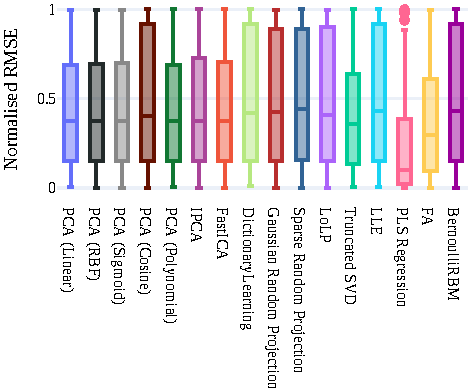
\includegraphics[width=\textwidth]{figures/05/epm/real_agg_sample_red_dim_1000_5.pdf}
        \caption{$N = 100, k=5$}
    \end{subfigure}
    \begin{subfigure}[t]{0.24\textwidth}
        \centering
        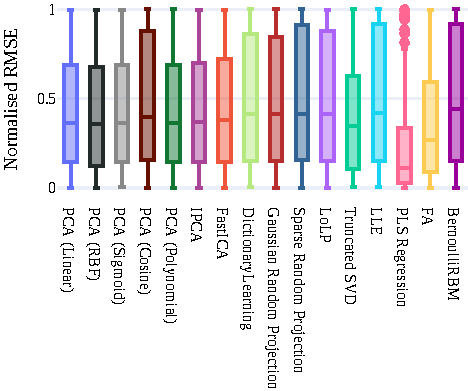
\includegraphics[width=\textwidth]{figures/05/epm/real_agg_sample_red_dim_1000_10.pdf}
        \caption{$N = 100, k=10$}
    \end{subfigure}
    \begin{subfigure}[t]{0.24\textwidth}
        \centering
        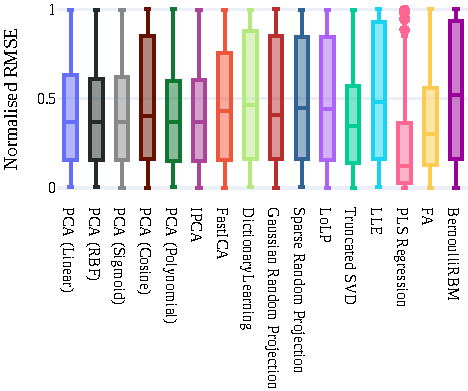
\includegraphics[width=\textwidth]{figures/05/epm/real_agg_sample_red_dim_1000_20.pdf}
        \caption{$N = 100, k=20$}
    \end{subfigure}
    \begin{subfigure}[t]{0.24\textwidth}
        \centering
        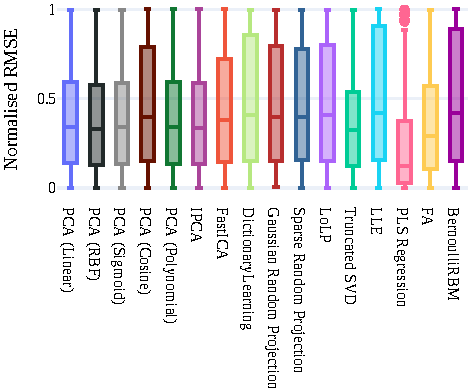
\includegraphics[width=\textwidth]{figures/05/epm/real_agg_sample_red_dim_1000_40.pdf}
        \caption{$N = 100, k=40$}
    \end{subfigure}
    \begin{subfigure}[t]{0.24\textwidth}
        \centering
        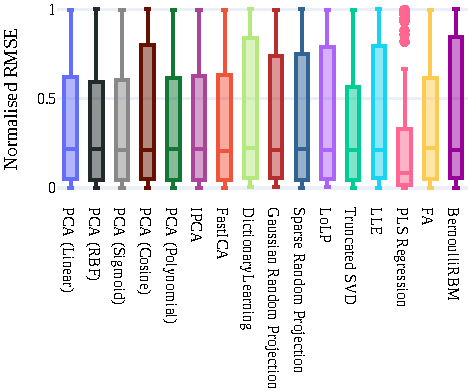
\includegraphics[width=\textwidth]{figures/05/epm/real_agg_sample_red_dim_100_5.pdf}
        \caption{$k = 5, N = 100$}
    \end{subfigure}
    \begin{subfigure}[t]{0.24\textwidth}
        \centering
        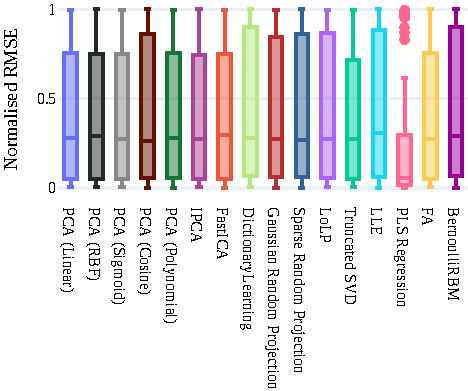
\includegraphics[width=\textwidth]{figures/05/epm/real_agg_sample_red_dim_200_5.pdf}
        \caption{$k = 5, N = 200$}
    \end{subfigure}
    \begin{subfigure}[t]{0.24\textwidth}
        \centering
        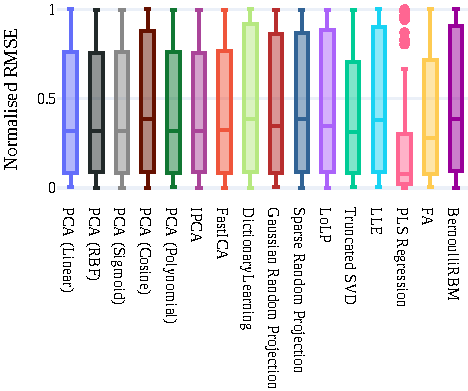
\includegraphics[width=\textwidth]{figures/05/epm/real_agg_sample_red_dim_500_5.pdf}
        \caption{$k = 5, N = 500$}
    \end{subfigure}
    \begin{subfigure}[t]{0.24\textwidth}
        \centering
        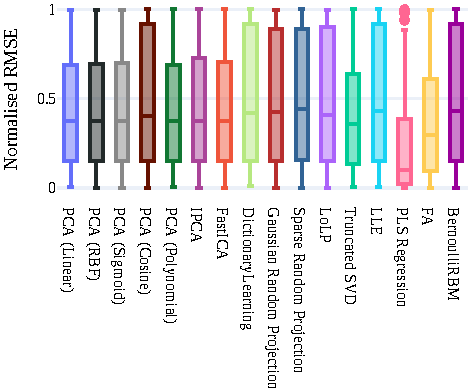
\includegraphics[width=\textwidth]{figures/05/epm/real_agg_sample_red_dim_1000_5.pdf}
        \caption{$k = 5, N = 1000$}
    \end{subfigure}
    % \hspace{0.2cm}
    % \begin{subfigure}[t]{0.8\textwidth}
    %     \centering
    %     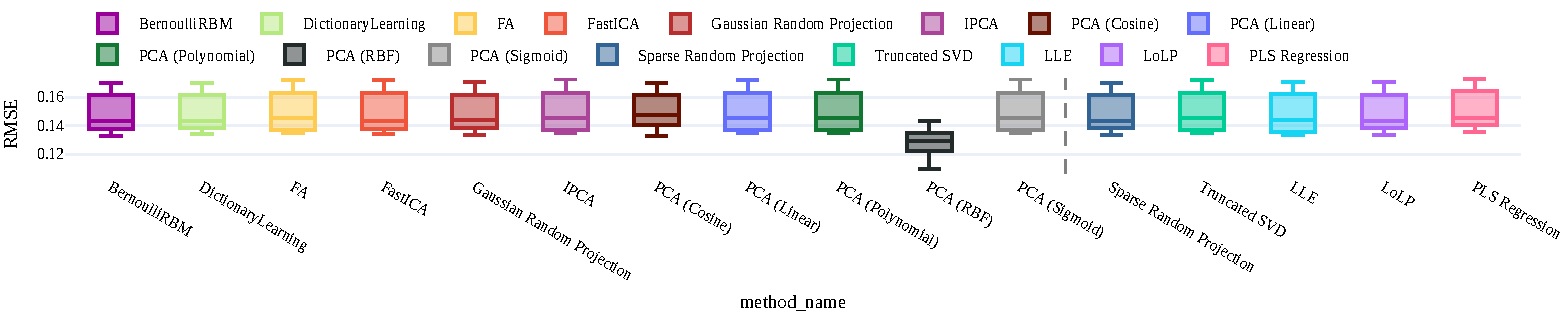
\includegraphics[width=1.0\textwidth,trim={1.5cm 4cm 3.7cm 0.0cm},clip]{figures/05/legend.pdf}
    % \end{subfigure}
    \caption{
    % \changed{
    Performance of different dimensionality reduction methods aggregated across real-world benchmark problems in two settings: (a-d) for different target dimensionalities $k$ with initial sample size $N = 100$, and (e-h) for different initial sample sizes $N$ with target dimensionality $k = 5$, in terms of min-max normalised mean \gls{rmse} on \textbf{black-box optimisation task 1: target function approximation}; lower is better.
    Note that the input dimensionality is determined by the benchmark and cannot be controlled.
    PLS regression outperforms other methods across all target dimensionalities even when the initial sample size is small.
    % Aggregated and min-max normalised mean ranks of the methods across all \emph{real-world} problems for different target dimensions with $100$ initial samples (a-d), different sample sizes and target dimension of 5 (e-h).}
    %\er{Why do we always have the outlier at the top?}
    % }
    % \todo{y-axis not mean ranks, but normalised RMSE}
    }
    \label{fig:res-bbo-task1_real}
\end{figure}

So far, our assessment has focused on synthetic benchmarks for black-box optimisation. \autoref{fig:res-bbo-task1_real} shows the results on real-world benchmarks. Figures (a–d) illustrate performance across varying target dimensionalities, with the initial sample size fixed at $N = 100$ (note that input dimensionality is determined by the benchmark and cannot be controlled). Across all target dimensionalities, PLS regression consistently outperforms other methods, reflecting its ability to extract components that are directly predictive of the target variables.
Figures (e–g) show the effect of varying the initial sample size while keeping the target dimensionality fixed at $k = 5$. Similar to the synthetic experiments, performance is relatively comparable across methods at smaller initial sample sizes, likely because most real-world benchmarks are high-dimensional, and small initial sample sizes limit the ability of the methods to extract reliable components. At an initial sample size of $N = 1000$, however, PLS regression clearly emerges as the best-performing method, confirming that adequate initial sample size is crucial for its predictive advantage in real-world, high-dimensional tasks.
% }

\subsubsection*{Black-box optimisation task 2: Optimiser performance}
% \changed{
We now focus on the results of black-box optimisation task 2, where Bayesian optimisation is assisted by the dimensionality reduction methods. As in the previous task, we vary the target dimensionality $k$, while fixing both the initial sample size to $N = 100$ and the original input dimensionality to $D = 120$. The aggregated results across all synthetic benchmark problems are shown in \autoref{fig:res-bbo-task2_red_dim}.
In contrast to the previous black-box optimisation task, PCA (RBF) consistently exhibits best performance across all target dimensionalities. Interestingly, PCA (Cosine) shows a noticeable improvement compared to its performance in the previous task, although it still falls short of PCA (RBF).
% \changed{
In contrast to relatively good performance of LLE in the machine learning task 1 (clustering ability), it is consistently the worst performing method in this task, closely followed by Bernoulli RBM for the highest target dimensionality.
% }
% \er{Sorry for the fundamental question here, but it seems a weird coincidence that PCA methods are the best performing and the weighting scheme was indeed thought for such dim red technique. Does the weighting scheme bias the performance?}

\begin{figure}
    \centering
    \begin{subfigure}[t]{0.24\textwidth}
        \centering
        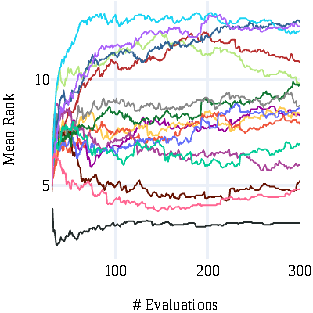
\includegraphics[width=\textwidth]{figures/05/bop/rank_100_120_5.pdf}
        \caption{$k=5$}
    \end{subfigure}
    \begin{subfigure}[t]{0.24\textwidth}
        \centering
        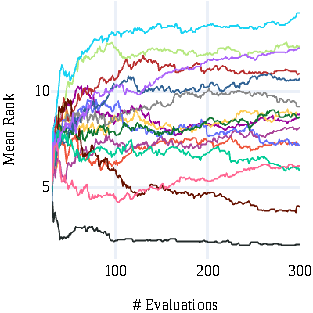
\includegraphics[width=\textwidth]{figures/05/bop/rank_100_120_10.pdf}
        \caption{$k=10$}
    \end{subfigure}
    \begin{subfigure}[t]{0.24\textwidth}
        \centering
        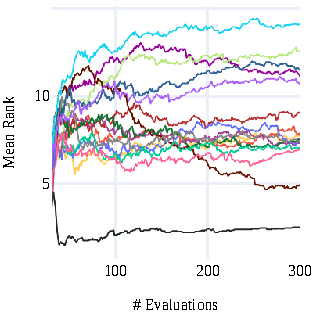
\includegraphics[width=\textwidth]{figures/05/bop/rank_100_120_20.pdf}
        \caption{$k=20$}
    \end{subfigure}
    \begin{subfigure}[t]{0.24\textwidth}
        \centering
        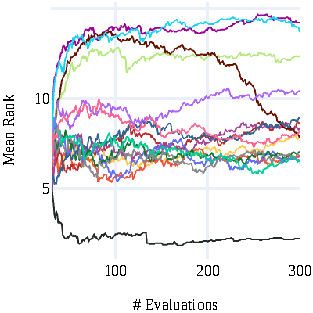
\includegraphics[width=\textwidth]{figures/05/bop/rank_100_120_40.pdf}
        \caption{$k=40$}
    \end{subfigure}
    \begin{subfigure}[t]{0.8\textwidth}
        \centering
        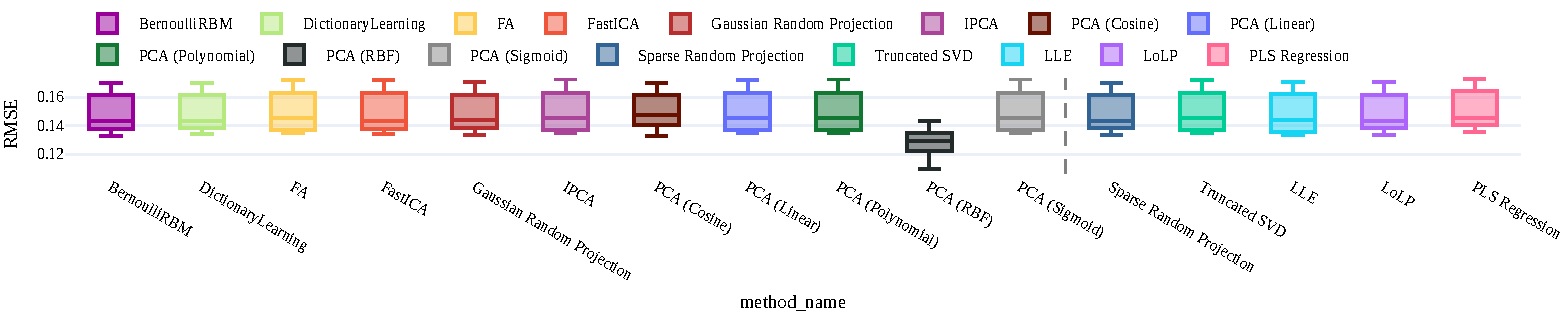
\includegraphics[width=1.0\textwidth,trim={1.5cm 4cm 3.7cm 0.0cm},clip]{figures/05/legend.pdf}
    \end{subfigure}
    \caption{
    % \changed{
    Performance of different dimensionality reduction methods aggregated across synthetic benchmark problems for different target dimensionalities $k$ with input dimensionality $D = 120$ and initial sample size $N = 100$, in terms of mean rank trajectories over the optimisation process on \textbf{black-box optimisation task 2: optimiser performance}; lower rank is better. 
    PCA (RBF) strongly outperforms all other methods across all target dimensionalities, followed by PLS regression and PCA (Cosine) for low target dimensionalities.
    LLE is the worst performing method, followed by Bernoulli RBM in the highest target dimensionality.
    % Ranks of the methods across all \emph{synthetic} problems for different target dimensions with $100$ initial samples.
    % }
    }
    \label{fig:res-bbo-task2_red_dim}
\end{figure}

Next, we analyse the effect of varying input dimensionalities $D$ while fixing the initial sample size at $N = 100$ and the target dimensionality at $k = 20$.~\autoref{fig:res-bbo-task2_diff_dims} shows the results aggregated across all synthetic benchmark problems. Across all input dimensionalities, PCA (RBF) consistently outperforms the other methods, confirming its robustness in this task.
Interestingly, unlike in black-box optimisation task 1 (target function approximation, which can also be seen as performance prediction from the point of view of empirical performance models~\citep{HutEtAl2014}), where PLS regression excelled at lower input dimensionalities, here it performs better on higher-dimensional inputs on average. This shift likely reflects the difference in task objectives: in Bayesian optimisation, capturing broader input-space structure becomes more important as dimensionality increases, allowing PLS regression to extract useful predictive directions even without low-dimensional constraints.
Additionally, PCA (Cosine) shows improved performance across all input dimensionalities compared to the previous task, though it still remains slightly below PCA (RBF), suggesting that kernel-based PCA variants generally benefit more from the unsupervised optimisation setting.
% \changed{
Last, LLE exhibits consistent poor performance, in line with the previous findings for this task.
% }

\begin{figure}
    \begin{subfigure}[t]{0.32\textwidth}
        \centering
        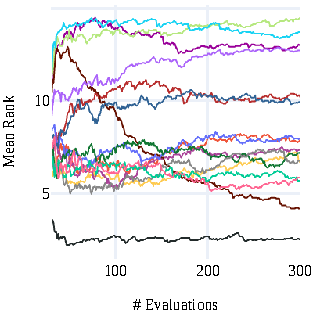
\includegraphics[width=\textwidth]{figures/05/bop/rank_100_40_20.pdf}
        \caption{$D=40$}
    \end{subfigure}
    \begin{subfigure}[t]{0.32\textwidth}
        \centering
        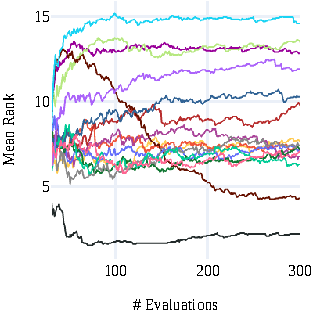
\includegraphics[width=\textwidth]{figures/05/bop/rank_100_60_20.pdf}
        \caption{$D=60$}
    \end{subfigure}
    \begin{subfigure}[t]{0.32\textwidth}
        \centering
        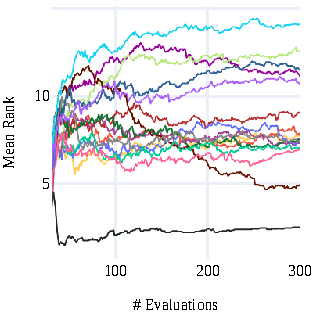
\includegraphics[width=\textwidth]{figures/05/bop/rank_100_120_20.pdf}
        \caption{$D=120$}
    \end{subfigure}
    \begin{subfigure}[t]{0.32\textwidth}
        \centering
        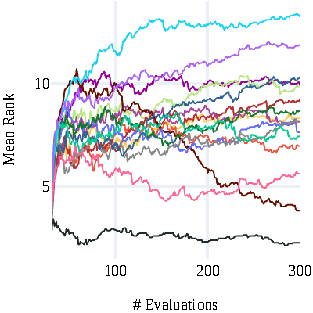
\includegraphics[width=\textwidth]{figures/05/bop/rank_100_240_20.pdf}
        \caption{$D=240$}
    \end{subfigure}
    \begin{subfigure}[t]{0.32\textwidth}
        \centering
        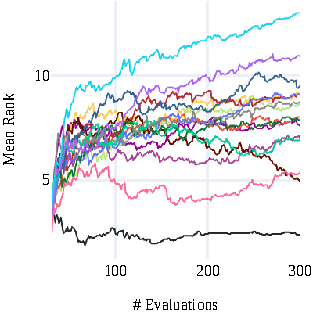
\includegraphics[width=\textwidth]{figures/05/bop/rank_100_500_20.pdf}
        \caption{$D=500$}
    \end{subfigure}
    \begin{subfigure}[t]{0.32\textwidth}
        \centering
        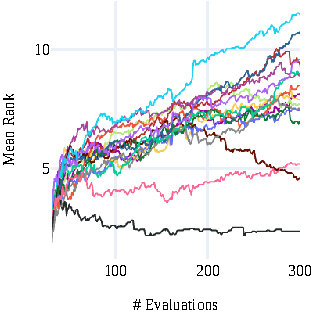
\includegraphics[width=\textwidth]{figures/05/bop/rank_100_1000_20.pdf}
        \caption{$D=1000$}
    \end{subfigure}
    \hspace{0.2cm}
    \begin{subfigure}[t]{0.8\textwidth}
        \centering
        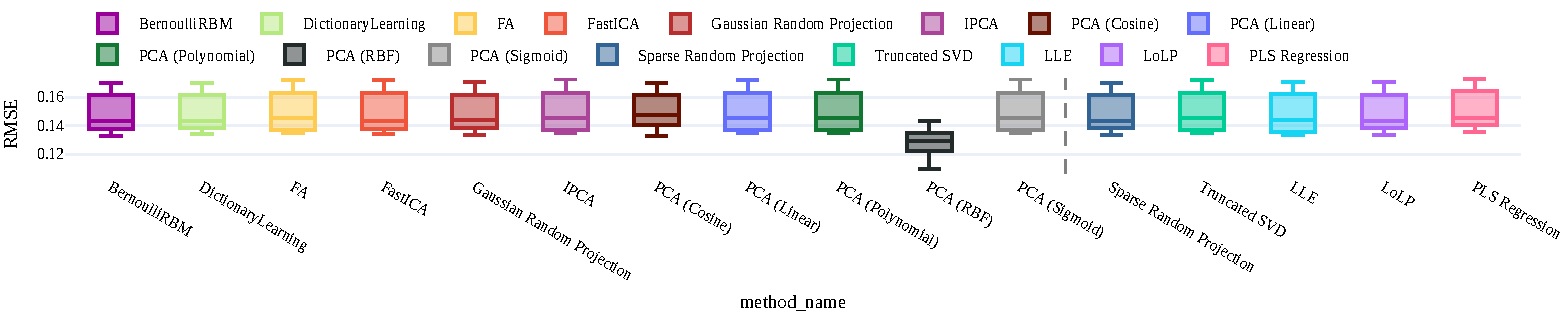
\includegraphics[width=1.0\textwidth,trim={1.5cm 4cm 3.7cm 0.0cm},clip]{figures/05/legend.pdf}
    \end{subfigure}
    \caption{
    % \changed{
    Performance of different dimensionality reduction methods aggregated across synthetic benchmark problems for different input dimensionalities $D$ with target dimensionality $k = 20$ and initial sample size $N = 100$, in terms of mean rank trajectories over the optimisation process on \textbf{black-box optimisation task 2: optimiser performance}; lower rank is better. 
    PCA (RBF) strongly dominates all other methods across all input dimensionalities, followed by PLS regression for high input dimensionalities.
    PCA (Cosine) rapidly catches up with the top-ranked methods for lower-dimensional inputs, outranking PLS regression for $D = 240$ in the last stage of the optimisation process, but still consistently failing to outperform PCA (RBF).
    LLE is the worst performing method, followed by dictionary learning and Bernoulli RBM for lower input dimensionalities.
    % Ranks of the methods across all \emph{synthetic} problems for different target dimensions with $100$ initial samples.
    % }
    }
    \label{fig:res-bbo-task2_diff_dims}
\end{figure}

We further examine the effect of varying initial sample sizes $N$ on performance, as shown in \autoref{fig:res-bbo-task2_samples}. Figures (a–d) correspond to low-dimensional inputs ($D = 40$) with target dimensionality fixed at $k = 5$. In this setting, PCA (RBF) generally performs best, although PCA (Cosine) competes closely at small initial sample sizes, suggesting that with limited data, the choice of kernel can influence the stability of the projection.
Figures (e–h) show the results for high-dimensional inputs ($D = 1000$) with target dimensionality fixed at $k = 40$. Here, PLS regression performs comparably to PCA (RBF) when the initial sample size is large, indicating that with sufficient data, supervised methods can extract predictive directions even in very high-dimensional spaces, narrowing the gap with unsupervised methods.
\begin{figure}
    \centering
    \begin{subfigure}[t]{0.24\textwidth}
        \centering
        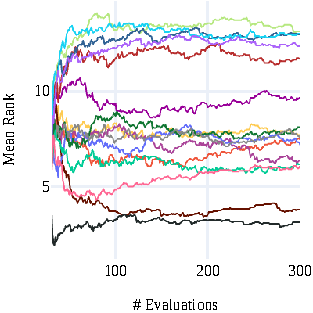
\includegraphics[width=\textwidth]{figures/05/bop/rank_100_40_5.pdf}
        \caption{\footnotesize$D = 40, k = 5, N = 100$}
    \end{subfigure}
    \begin{subfigure}[t]{0.24\textwidth}
        \centering
        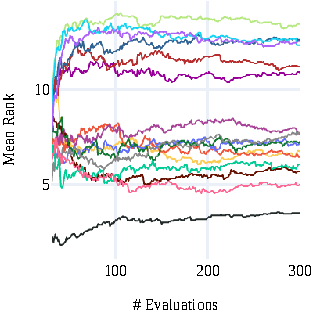
\includegraphics[width=\textwidth]{figures/05/bop/rank_200_40_5.pdf}
        \caption{\footnotesize$D = 40, k = 5, N = 200$}
    \end{subfigure}
    \begin{subfigure}[t]{0.24\textwidth}
        \centering
        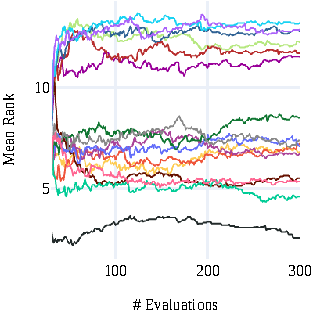
\includegraphics[width=\textwidth]{figures/05/bop/rank_500_40_5.pdf}
        \caption{\footnotesize$D = 40, k = 5, N = 500$}
    \end{subfigure}
    \begin{subfigure}[t]{0.24\textwidth}
        \centering
        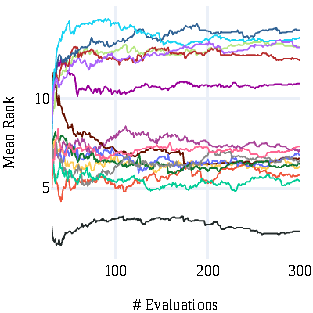
\includegraphics[width=\textwidth]{figures/05/bop/rank_1000_40_5.pdf}
        \caption{\footnotesize$D = 40, k = 5, N = 1000$}
    \end{subfigure}
    \begin{subfigure}[t]{0.24\textwidth}
        \centering
        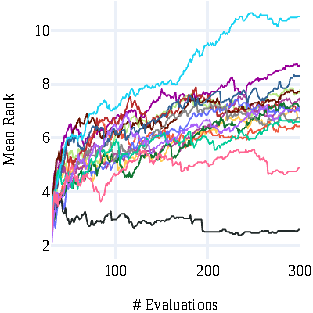
\includegraphics[width=\textwidth]{figures/05/bop/rank_100_1000_40.pdf}
        \caption{\footnotesize$D = 1000, k = 40, N = 100$}
    \end{subfigure}
    \begin{subfigure}[t]{0.24\textwidth}
        \centering
        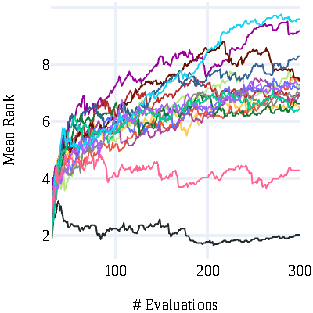
\includegraphics[width=\textwidth]{figures/05/bop/rank_200_1000_40.pdf}
        \caption{\footnotesize$D = 1000, k = 40, N = 200$}
    \end{subfigure}
    \begin{subfigure}[t]{0.24\textwidth}
        \centering
        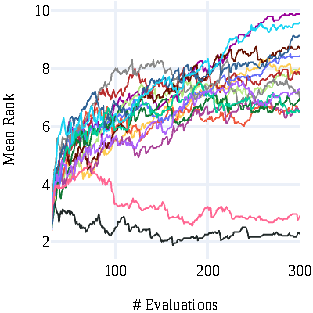
\includegraphics[width=\textwidth]{figures/05/bop/rank_500_1000_40.pdf}
        \caption{\footnotesize$D = 1000, k = 40, N = 500$}
    \end{subfigure}
    \begin{subfigure}[t]{0.24\textwidth}
        \centering
        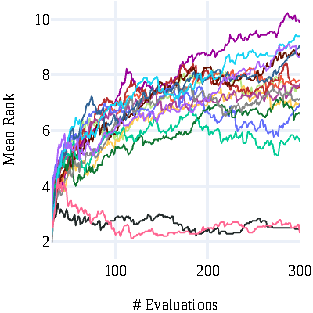
\includegraphics[width=\textwidth]{figures/05/bop/rank_1000_1000_40.pdf}
        \caption{\footnotesize$D = 1000, k = 40, N = 1000$}
    \end{subfigure}
    \hspace{0.2cm}
    \begin{subfigure}[t]{0.8\textwidth}
        \centering
        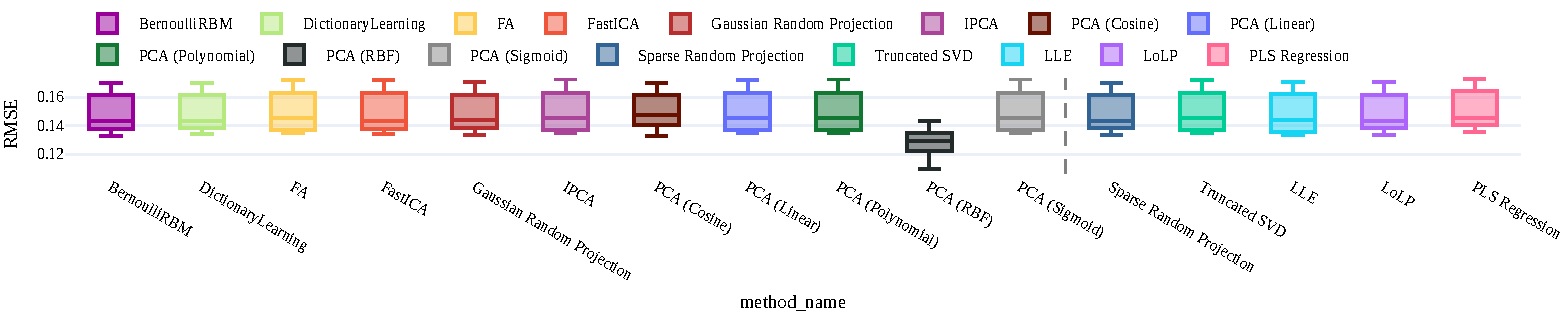
\includegraphics[width=1.0\textwidth,trim={1.5cm 4cm 3.7cm 0.0cm},clip]{figures/05/legend.pdf}
    \end{subfigure}
    \caption{
    % \changed{
    Performance of different dimensionality reduction methods aggregated across synthetic benchmark problems for different initial sample sizes $N$ in two settings: (a-d) with input dimensionality $D = 40$ and target dimensionality $k = 5$, and (e-h) with input dimensionality $D = 1000$ and target dimensionality $k = 40$, in terms of mean rank trajectories over the optimisation process on \textbf{black-box optimisation task 2: optimiser performance}; lower rank is better.
    PCA (RBF) is the top-ranked method across both settings, while PLS regression exhibits stronger performance for high-dimensional inputs than for low-dimensional ones.
    Dictionary learning, LLE, Bernoulli RBM and PCA (Cosine) are among the worst performers for low-dimensional inputs, whereas for high input dimensionalities, LLE stands out with its poor performance when the initial sample size is low, but quickly becomes indistinguishable from, \emph{e.g.,}, Bernoulli RBM (and other methods) as the initial sample size increases.
    % Ranks of the methods across all \emph{synthetic} problems for different initial sample sizes with target dimension $5$ and input dimension $40$ (a-d) and $1000$ (e-h).
    % }
    }
    \label{fig:res-bbo-task2_samples}
\end{figure}

% \changed{
Finally, we look into the results on real-world benchmark problems in~\autoref{fig:res-bbo-task2-real-world}, which paint a considerably different picture than synthetic benchmarks.
In Figures (a-d) we investigate the impact of varying target dimensionality $k$ while keeping the initial sample size fixed at $N = 100$. 
Unlike synthetic benchmarks where higher value of target dimensionality allowed for a relatively consistent performance improvement, here we see more complex optimisation dynamics, with highly variable performance across methods.
At the lowest target dimensionality we observe the most diverse performance of all methods, and the rapid convergence followed by plateaus suggests that most of the intrinsic information in dimension $5$ is captured early on in the optimisation process.
When target dimensionality is increased from $k = 20$ to $k = 40$, performance does not drastically improve, even though the advantage of methods that exhibited good performance for low values of $k$ diminishes.
This suggests that real-world optimisation problems may have intrinsic dimensionality in the range of $10$ to $20$ dimensions that are effectively exploitable (even with a small initial sample size of $100$), while additional target dimensions yield limited benefit and can even make the optimisation process more challenging.
Notably, for different target dimensionalities we cannot distinguish a clear winner among dimensionality reduction methods, while LLE is especially ill-suited for higher values of $k$ on this task.

Last, we assess the impact of varying initial sample sizes $N$ while keeping the target dimensionality fixed at $k = 5$ in Figures (e-h). 
Most methods start off with strong fluctuations in their convergence curves at the smallest initial sample size, suggesting that an insufficient amount of training data leads to unreliable dimensionality reduction mapping.
As the initial sample size increases, the convergence curves become smoother and more regular, and the performance gap between two distinct sets of methods becomes apparent.
Among good performers, we find in particular all PCA variants (with a notable exception of PCA (Cosine)), and PLS regression (which is top-ranked for the initial sample size of $N = 200$, and showed a consistent strong performance in the previous black-box optimisation task, as well as in this task on synthetic benchmarks).
Poor performance was yielded by LLE, Bernoulli RBM, LoLP, Gaussian and sparse random projections, dictionary learning, and, surprisingly, PCA (Cosine), which was often among the three top-ranked dimensionality reduction methods on synthetic benchmarks in this task.
The results indicate that the initial sample size used for training dimensionality reduction methods critically affects both optimisation quality and smoothness of convergence in real-world scenarios.
Moreover, as real-world function evaluations are expensive, this highlights a trade-off in allocating evaluations for training dimensionality reduction methods and for running the optimiser itself.

Overall, stark differences between performances of the methods on synthetic vs. real-world benchmarks likely reflect the heterogeneous nature of real-world problems, where features defining the search space often come from various domains and have complex interactions.
Across almost all considered settings, there is an evident tendency for methods to plateau well before the full optimisation budget is exhausted, causing the performance to stagnate.
This might indicate that, on real-world problems, the optimiser assisted by dimensionality reduction can effectively exploit only the global structure preserved in the reduced space, but loses access to more fine-grained details of these complex landscapes.
Finally, through high variability of observed behaviours across all settings, we see a general pattern of performance complementarity of different dimensionality reduction methods; while some methods excel on some problems, they perform poorly on others. 

% }

% \todo{}
% \hh{What's with these todo items?}

\begin{figure}
    \centering
    \begin{subfigure}[t]{0.24\textwidth}
        \centering
        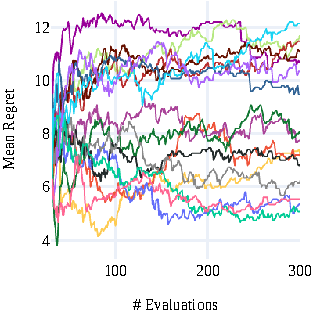
\includegraphics[width=\textwidth]{figures/05/bop/rank_real_100_5.pdf}
        \caption{$N = 100, k = 5$}
    \end{subfigure}
    \begin{subfigure}[t]{0.24\textwidth}
        \centering
        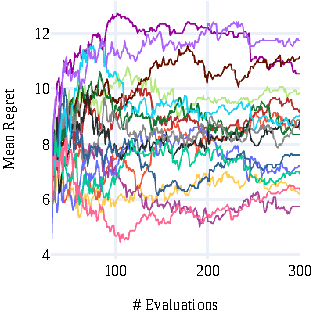
\includegraphics[width=\textwidth]{figures/05/bop/rank_real_100_10.pdf}
        \caption{$N = 100, k = 10$}
    \end{subfigure}
    \begin{subfigure}[t]{0.24\textwidth}
        \centering
        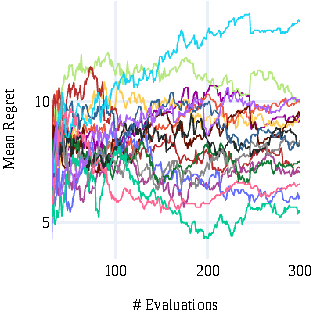
\includegraphics[width=\textwidth]{figures/05/bop/rank_real_100_20.pdf}
        \caption{$N = 100, k = 20$}
    \end{subfigure}
    \begin{subfigure}[t]{0.24\textwidth}
        \centering
        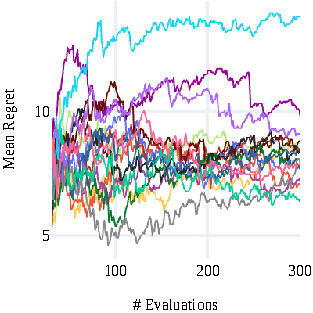
\includegraphics[width=\textwidth]{figures/05/bop/rank_real_100_40.pdf}
        \caption{$N = 100, k = 40$}
    \end{subfigure}
    \begin{subfigure}[t]{0.24\textwidth}
        \centering
        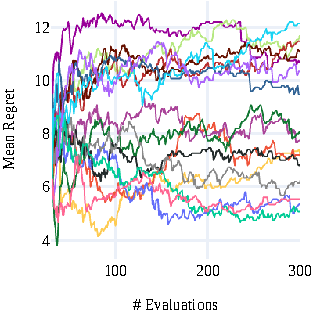
\includegraphics[width=\textwidth]{figures/05/bop/rank_real_100_5.pdf}
        \caption{$k = 5, N = 100$}
    \end{subfigure}
    \begin{subfigure}[t]{0.24\textwidth}
        \centering
        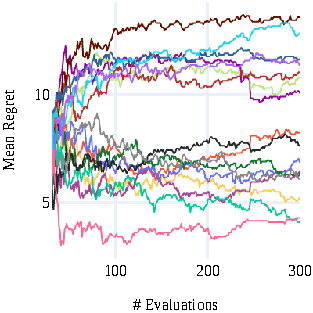
\includegraphics[width=\textwidth]{figures/05/bop/rank_real_200_5.pdf}
        \caption{$k = 5, N = 200$}
    \end{subfigure}
    \begin{subfigure}[t]{0.24\textwidth}
        \centering
        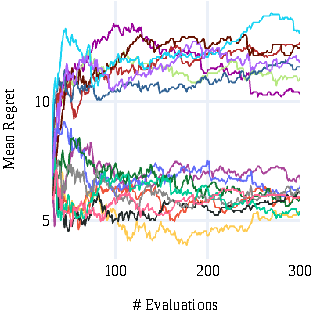
\includegraphics[width=\textwidth]{figures/05/bop/rank_real_500_5.pdf}
        \caption{$k = 5, N = 500$}
    \end{subfigure}
    \begin{subfigure}[t]{0.24\textwidth}
        \centering
        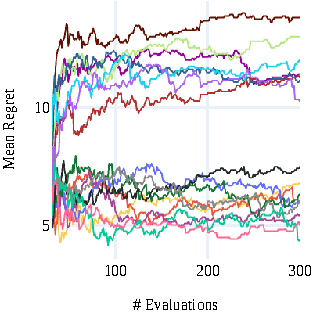
\includegraphics[width=\textwidth]{figures/05/bop/rank_real_1000_5.pdf}
        \caption{$k = 5, N = 1000$}
    \end{subfigure}
    \hspace{0.2cm}
    \begin{subfigure}[t]{0.8\textwidth}
        \centering
        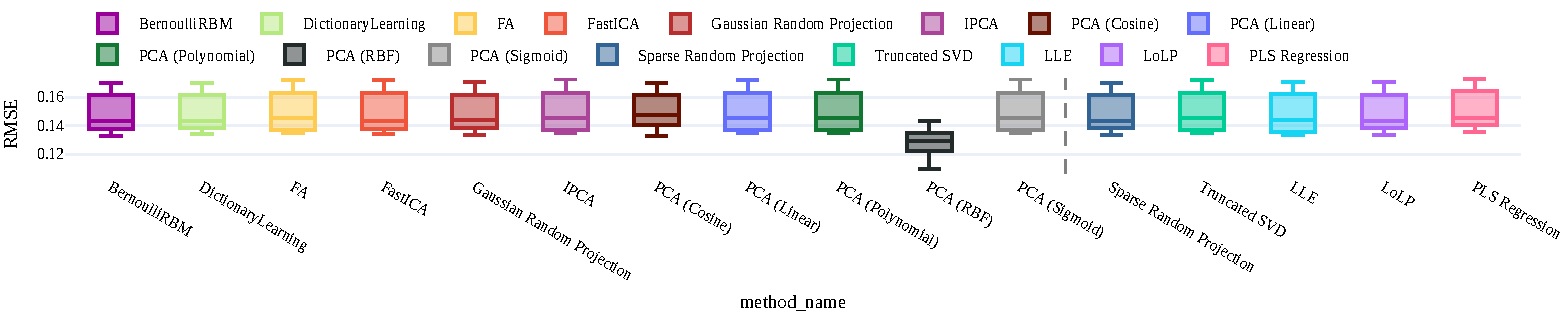
\includegraphics[width=1.0\textwidth,trim={1.5cm 4cm 3.7cm 0.0cm},clip]{figures/05/legend.pdf}
    \end{subfigure}
    \caption{
    % \changed{
    Performance of different dimensionality reduction methods aggregated across real-world benchmark problems in two settings: (a-d) for different target dimensionalities $k$ with initial sample size $N = 100$, and (e-h) for different initial sample sizes $N$ with target dimensionality $k = 5$, in terms of mean rank trajectories over the optimisation process on \textbf{black-box optimisation task 2: optimiser performance}; lower rank is better. Note that (i) the input dimensionality is determined by the benchmark and cannot be controlled, and (ii) figures (a) and (e) correspond to the same scenario.
    In the first setting, there is no single top-ranked method; LLE stands out as the worst performing method for higher target dimensionalities.
    In the second setting, as the number of initial samples grows, there appears a substantial spread in performance between two distinct sets of methods; notably, PCA (Cosine) is among the worst performers.
    % Ranks of the methods across all \emph{real-world} problems for different initial target dimensions with with initial sample size of $100$(a-d) and different sample sizes and target dimension of $5$ (e-h).
    % }
    }
    \label{fig:res-bbo-task2-real-world}
\end{figure}

% }
\section{Running times}
\label{sec:rt}

% \changed{
In~\autoref{fig:res-rt} we present the training and transformation running times of the dimensionality reduction methods for 2 selected OpenML datasets 
% \changed{
used in machine learning tasks 1 and 2: one with a lower dimensionality and a high number of elements, and one with a higher dimensionality and a low number of elements.
% }
The running times are reported as CPU time.
We note that we report the transformation time 
% \changed{
needed for the two machine learning tasks,
% for ML datasets, 
but the times for black-box optimisation task 1 are similar 
as in this task we simply train and transform on a fixed dataset.
% \aj{I don't like that we only say similar without any evidence to support it. It might be good to elaborate a bit on this}. 
For black-box optimisation task 2, it is 
% harder 
more challenging to isolate
% to compute 
the effect of the running time of the dimensionality reduction itself, as it is 
% part of 
integrated in
the surrogate training and acquisition function optimisation, which are additional factors that can greatly affect the total running time.

We observe that for both training and transformation of low-dimensional datasets with a high number of elements (Figures (a-b)), LLE and PCA variants with non-linear kernels exhibit the highest running times.
% \changed{followed by dictionary learning for the transformation time}. 
For the high-dimensional dataset with a low number of elements (Figures (c-d)), the running times of those methods is lower compared to most other methods. In this setting, dictionary learning is the most expensive method in terms of running time.
% \changed{
We observe that Gaussian and sparse random projections consistently incur low running times, and that PLS regression is quite competitive in this regard for both datasets.
% }


\begin{figure}
    \centering
    \begin{subfigure}[t]{0.24\textwidth}
        \centering
        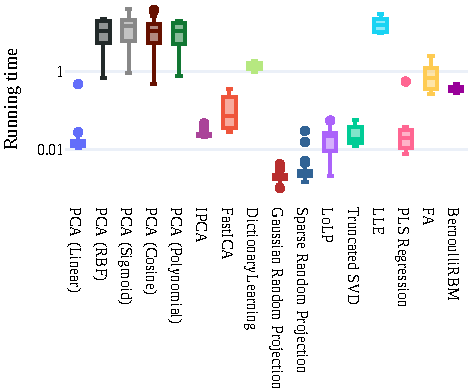
\includegraphics[width=\textwidth]{figures/05/time/9985_train_time.pdf}
        \caption{Training on dataset 9985}
    \end{subfigure}
    \begin{subfigure}[t]{0.24\textwidth}
        \centering
        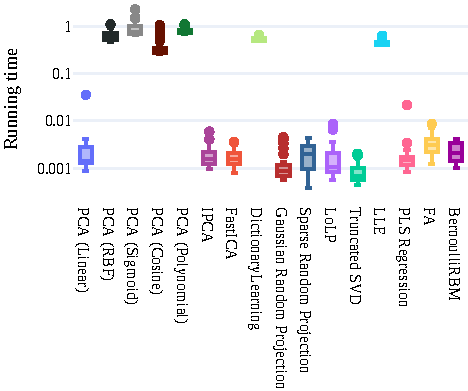
\includegraphics[width=\textwidth]{figures/05/time/9985_transform_time.pdf}
        \caption{Transform on dataset 9985}
    \end{subfigure}
        \begin{subfigure}[t]{0.24\textwidth}
        \centering
        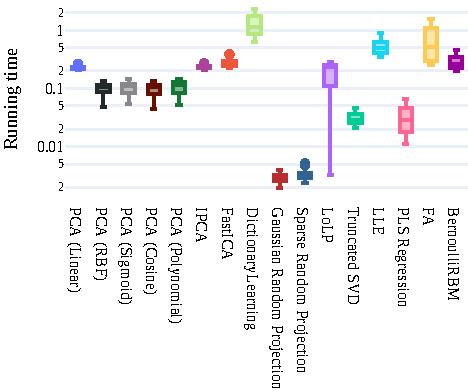
\includegraphics[width=\textwidth]{figures/05/time/9981_train_time.pdf}
        \caption{Train on dataset 9981}
    \end{subfigure}
    \begin{subfigure}[t]{0.24\textwidth}
        \centering
        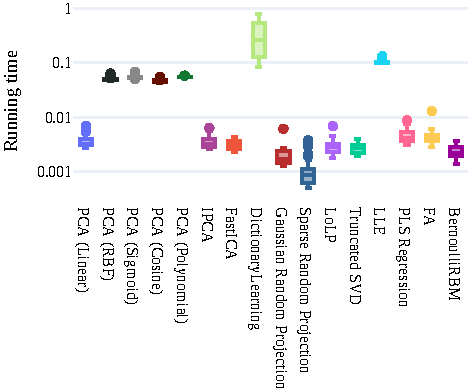
\includegraphics[width=\textwidth]{figures/05/time/9981_transform_time.pdf}
        \caption{Transform on dataset 9981}
    \end{subfigure}
    \caption{
    % \changed{
    Running times in terms of CPU hours for dimensionality reduction training (a, c) and transformation (b, d) of OpenML datasets 9985 (51 features and 6618 elements) and 9981 (856 features and 1080 elements).
    % }
    }
    \label{fig:res-rt}
\end{figure}

% }

\section{Discussion}
\label{sec:disc}

% \changed{
Our comprehensive assessment of dimensionality reduction methods reveals fundamental differences in how the benchmarked methods perform in machine learning and black-box optimisation contexts.
An important insight of this study is the existence of strong task-dependent performance complementarity, as no single dimensionality reduction method dominates across all tasks.
This observation underscores that, to achieve best possible performance, proper method selection must be task-driven.

In the machine learning domain, we observed relatively similar performance of most dimensionality reduction methods.
For clustering, most methods struggled to preserve cluster homogeneity, indicating that class boundaries are challenging to capture, while cluster completeness was successfully retained by random projection methods and LLE in higher-dimensional subspaces.
In particular, good performance of LLE in this context may be due to its unsupervised nature and the fact it is designed to capture local structure.
Interestingly, this very characteristic of LLE might be responsible for its poor performance in assisting an optimiser.
For classification, most methods achieved a consistently high accuracy regardless of the underlying machine learning model (with the exception of random projections and Bernoulli RBM), suggesting that for well-structured tabular data, the choice of dimensionality reduction method has limited impact on downstream classification performance.
Both machine learning tasks showed that performance improves monotonically with target dimensionality, meaning that higher-dimensional projections retain more task-relevant information for structured datasets.

On the other hand, in the black-box optimisation domain, the choice of dimensionality reduction method had a substantial impact on the downstream performance, due to strong performance differences between methods.
For target function approximation, PLS regression was a top performer at lower target dimensionalities and moderate input dimensionalities, in line with the fact that it is a supervised method designed with the objective of extracting components directly predictive of function values.
However, for very-high dimensional inputs, or for insufficient data for training dimensionality reduction methods, PCA with the RBF kernel overtook PLS regression as the top-performing method.
A reason for this might be that unsupervised variance-based methods supported by an adequate non-linear kernel are able to capture essential problem structure when the original search space is extremely large and/or not well covered.

% \changed{
For optimiser performance, PCA with the RBF kernel excels by a large margin in assisting Bayesian optimisation in high-dimensional spaces.
This indicates that, in order to successfully perform Bayesian optimisation in the reduced space, dimensionality reduction has to be done via methods that preserve the global geometric structure of the objective function, and not merely predictive components.
For instance, LLE consistently performed worst in this task, showing that preserving local (instead of global) structure is detrimental for assisting optimisation procedures.
% Notably,  performed considerably worse in this task compared to target function approximation.
% While PCA with the RBF kernel has also been shown to perform well in approximating the black-box target functions, it is outperformed for this task by another prominent method, namely PLS regression.
In particular, PLS regression (which was top-ranked for target function approximation) is not able to outperform PCA with the RBF kernel here.
Intuitively, this is because accurate prediction of function values does not necessarily translate to effective (and efficient) optimisation, as already observed in~\citep{FeuEtAl18}. %\aj{do we need to cite?}
In other words, problem characteristics required for guiding the search process fundamentally differ from those allowing for accurate function value regression, and the strong performance of PCA with the RBF kernel specifically suggests that capturing non-linear, distance-based relationships in the search space is crucial for optimisation, more so than explicit supervision on objective values.

We note that different sample sizes for training dimensionality reduction methods were used for the two black-box optimisation tasks.
However, as target function approximation via a surrogate model is a key component of Bayesian optimisation, we conjecture that some methods would tend to be effective in enhancing the optimiser, even if the surrogate (in the Bayesian optimisation loop of black-box optimisation task 2) is fitted on a smaller sample than for target function approximation of  black-box optimisation task 1.
We believe these observations to be of great importance for designing out-of-the-box robust Bayesian optimisation-based approaches to tackle high-dimensional real-world problems.
% }
% For optimiser performance, PCA with the RBF kernel consistently and substantially outperformed all other methods across almost all settings.




% We saw in particular that principal component analysis (PCA) with the RBF kernel excels by a large margin in assisting Bayesian optimisation in high-dimensional spaces.
% While this method has also been shown to perform well in approximating the black-box target functions, it is outperformed by another prominent method, namely partial least squares (PLS) regression. 
% In our setup, we used different sample sizes for training dimensionality reduction methods for these two tasks.
% However, as target function approximation via a surrogate model is a key component of Bayesian optimisation, we conjecture that some methods would tend to be effective in enhancing the optimiser, even if the surrogate (in the Bayesian optimisation loop of  black-box optimisation Task 2) is fitted on a smaller sample than for target function approximation of  black-box optimisation Task 1.
% We believe these observations to be of great importance for designing out-of-the-box robust Bayesian optimisation-based approaches to tackle high-dimensional real-world problems.

% Finally, an important consideration on the dominance of PCA with the RBF kernel in the optimiser performance task is the fact that the Gaussian process surrogate from our chosen implementation of Bayesian optimisation uses the very same type of kernel.
% \aj{The following is now commented because it is obviously not completely correct, but it would be interesting to add something along those lines.}
% When we reduce dimensionality, we preserve distances and non-linear relationships between points in the reduced space in the same way our Gaussian process surrogate captures them, thereby enabling maximal exploitation of the underlying problem structure.
Taken together, these findings suggest that the task objective strongly shapes which dimensionality reduction method is most effective: supervised tasks favour methods aligned with predictive power, while unsupervised tasks benefit from methods that preserve geometric or topological structure.
% }
% \todo{add discussion on high-dimensional BO (ALEBO, BAxUS, HeSBO, SAASBO, TuRBO, RPM-BO); important to emphasise that we do not propose doing HDBO with DR, and that we do not argue that DR-assisted BO is the best alternative for HDBO, we are really only interested in seeing how much each DR method can help HDBO}


% The methods behave very differently depending on the context. What works for ML might not work for BBO and vice versa. Varying target dimensionality affects the methods differently depending on the use-case. 

% Taken together, our results highlight an important distinction between supervised and unsupervised dimensionality reduction. In the predictive task (black-box optimisation task 1), PLSRegression excels at low target dimensions because it explicitly optimises components for predicting the target variables, while PCA variants only match its performance once the target dimension is sufficiently high, allowing them to retain sufficient variance and structure for effective prediction. In contrast, in the clustering experiments, which are unsupervised, methods that preserve local structure (e.g., LLE) or capture non-linear relationships (e.g., PCA with RBF or Cosine kernels) tend to perform better. Random projection methods, particularly at higher dimensions, also show improvements due to the Johnson–Lindenstrauss effect, which preserves pairwise distances and cluster structure. Overall, these findings suggest that the task objective strongly shapes which dimensionality reduction method is most effective: supervised tasks favour methods aligned with predictive power, while unsupervised tasks benefit from methods that preserve geometric or topological structure.

% \er{Sorry for the fundamental question here, but it seems a weird coincidence that PCA methods are the best performing and the weighting scheme was indeed thought for such dim red technique. Does the weighting scheme bias the performance?}

\section{Conclusions and future work}
\label{sec:concl}

% \hh{modified:}
% \changed{
In this work, we assessed the performance of a broad range of dimensionality reduction methods based on four carefully chosen downstream tasks from two different fields: machine learning and black-box optimisation.
Each task allows for empirically evaluating different aspects of dimensionality reduction methods, highlighting the task-dependent differences in their performance.
Specifically, we conducted a thorough benchmarking study of 16 dimensionality reduction methods 
% \hh{do we really need the following remark? don't all dimensionality reduction techniques rely on feature extraction?}
(based on feature extraction) 
on these four tasks across a range of different settings (\emph{i.e.,} original dimensionality, target dimensionality, budget available for training dimensionality reduction methods), 
% \changed{
and derived practical insights into their suitability depending on their intended use.
% }
% In this paper we present novel tasks to assess the peformance of dimensionality reduction methods across two different fields: BBO and ML. 
% We design four different tasks, two for each use-case to assess the different aspects of dimensionality reduction. 
% Each task is tests different aspects of the methods.
% We also check the performance of the methods reducing to different dimensions.

% \changed{
In general, 
% }
we observed that the choice of dimensionality reduction method depends on the task, as for each of the four tasks, different methods perform best. 
% \hh{slightly modified:}
Moreover, even within the same task, different methods work best for different datasets or functions. 
% \changed{
While the performance differences are more prominent in  black-box optimisation tasks than in machine learning ones,
% }
this shows that there is \textit{performance complementarity}~\cite{Rice76,FreEtAl16} between the dimensionality reduction methods, and that careful method selection is of key importance for achieving optimal performance.
In practice, dimensionality reduction methods are typically chosen based on good performance in similar scenarios.
% \hh{modified:}
We expect that meta-learning which method to use in which case can yield substantial performance gains and intend to further pursue research in this direction in future work.

% \changed{

% Despite the differences in sample sizes used for training dimensionality reduction methods for the two black-box optimisation tasks, we found which methods tend to perform well even if we fit the surrogate on a smaller sample (within bo loop)

% We provide several guidelines to choose the dimensionality reduction method

% \hh{modified -- see whether you like it:}
Overall, dimensionality reduction methods often play a crucial role for solving problems in high-dimensional spaces. 
Our work presented here produced new insights on how these methods work in four broadly interesting scenarios, thus facilitating better understanding of their strengths and weaknesses. These insights can be used in the future to help design new and improve existing dimensionality reduction methods for specific tasks.